\documentclass[twoside]{book}

% Packages required by doxygen
\usepackage{fixltx2e}
\usepackage{calc}
\usepackage{doxygen}
\usepackage[export]{adjustbox} % also loads graphicx
\usepackage{graphicx}
\usepackage[utf8]{inputenc}
\usepackage{makeidx}
\usepackage{multicol}
\usepackage{multirow}
\PassOptionsToPackage{warn}{textcomp}
\usepackage{textcomp}
\usepackage[nointegrals]{wasysym}
\usepackage[table]{xcolor}

% Font selection
\usepackage[T1]{fontenc}
\usepackage[scaled=.90]{helvet}
\usepackage{courier}
\usepackage{amssymb}
\usepackage{sectsty}
\renewcommand{\familydefault}{\sfdefault}
\allsectionsfont{%
  \fontseries{bc}\selectfont%
  \color{darkgray}%
}
\renewcommand{\DoxyLabelFont}{%
  \fontseries{bc}\selectfont%
  \color{darkgray}%
}
\newcommand{\+}{\discretionary{\mbox{\scriptsize$\hookleftarrow$}}{}{}}

% Page & text layout
\usepackage{geometry}
\geometry{%
  a4paper,%
  top=2.5cm,%
  bottom=2.5cm,%
  left=2.5cm,%
  right=2.5cm%
}
\tolerance=750
\hfuzz=15pt
\hbadness=750
\setlength{\emergencystretch}{15pt}
\setlength{\parindent}{0cm}
\setlength{\parskip}{3ex plus 2ex minus 2ex}
\makeatletter
\renewcommand{\paragraph}{%
  \@startsection{paragraph}{4}{0ex}{-1.0ex}{1.0ex}{%
    \normalfont\normalsize\bfseries\SS@parafont%
  }%
}
\renewcommand{\subparagraph}{%
  \@startsection{subparagraph}{5}{0ex}{-1.0ex}{1.0ex}{%
    \normalfont\normalsize\bfseries\SS@subparafont%
  }%
}
\makeatother

% Headers & footers
\usepackage{fancyhdr}
\pagestyle{fancyplain}
\fancyhead[LE]{\fancyplain{}{\bfseries\thepage}}
\fancyhead[CE]{\fancyplain{}{}}
\fancyhead[RE]{\fancyplain{}{\bfseries\leftmark}}
\fancyhead[LO]{\fancyplain{}{\bfseries\rightmark}}
\fancyhead[CO]{\fancyplain{}{}}
\fancyhead[RO]{\fancyplain{}{\bfseries\thepage}}
\fancyfoot[LE]{\fancyplain{}{}}
\fancyfoot[CE]{\fancyplain{}{}}
\fancyfoot[RE]{\fancyplain{}{\bfseries\scriptsize Generated by Doxygen }}
\fancyfoot[LO]{\fancyplain{}{\bfseries\scriptsize Generated by Doxygen }}
\fancyfoot[CO]{\fancyplain{}{}}
\fancyfoot[RO]{\fancyplain{}{}}
\renewcommand{\footrulewidth}{0.4pt}
\renewcommand{\chaptermark}[1]{%
  \markboth{#1}{}%
}
\renewcommand{\sectionmark}[1]{%
  \markright{\thesection\ #1}%
}

% Indices & bibliography
\usepackage{natbib}
\usepackage[titles]{tocloft}
\setcounter{tocdepth}{3}
\setcounter{secnumdepth}{5}
\makeindex

% Hyperlinks (required, but should be loaded last)
\usepackage{ifpdf}
\ifpdf
  \usepackage[pdftex,pagebackref=true]{hyperref}
\else
  \usepackage[ps2pdf,pagebackref=true]{hyperref}
\fi
\hypersetup{%
  colorlinks=true,%
  linkcolor=blue,%
  citecolor=blue,%
  unicode%
}

% Custom commands
\newcommand{\clearemptydoublepage}{%
  \newpage{\pagestyle{empty}\cleardoublepage}%
}

\usepackage{caption}
\captionsetup{labelsep=space,justification=centering,font={bf},singlelinecheck=off,skip=4pt,position=top}

%===== C O N T E N T S =====

\begin{document}

% Titlepage & ToC
\hypersetup{pageanchor=false,
             bookmarksnumbered=true,
             pdfencoding=unicode
            }
\pagenumbering{roman}
\begin{titlepage}
\vspace*{7cm}
\begin{center}%
{\Large Py\+G\+CE \\[1ex]\large 0.\+1 }\\
\vspace*{1cm}
{\large Generated by Doxygen 1.8.11}\\
\end{center}
\end{titlepage}
\clearemptydoublepage
\tableofcontents
\clearemptydoublepage
\pagenumbering{arabic}
\hypersetup{pageanchor=true}

%--- Begin generated contents ---
\chapter{Namespace Index}
\section{Namespace List}
Here is a list of all namespaces with brief descriptions\+:\begin{DoxyCompactList}
\item\contentsline{section}{\hyperlink{namespacepygce}{pygce} }{\pageref{namespacepygce}}{}
\item\contentsline{section}{\hyperlink{namespacepygce_1_1analysis}{pygce.\+analysis} }{\pageref{namespacepygce_1_1analysis}}{}
\item\contentsline{section}{\hyperlink{namespacepygce_1_1analysis_1_1cli}{pygce.\+analysis.\+cli} }{\pageref{namespacepygce_1_1analysis_1_1cli}}{}
\item\contentsline{section}{\hyperlink{namespacepygce_1_1analysis_1_1models}{pygce.\+analysis.\+models} }{\pageref{namespacepygce_1_1analysis_1_1models}}{}
\item\contentsline{section}{\hyperlink{namespacepygce_1_1cli}{pygce.\+cli} }{\pageref{namespacepygce_1_1cli}}{}
\item\contentsline{section}{\hyperlink{namespacepygce_1_1models}{pygce.\+models} }{\pageref{namespacepygce_1_1models}}{}
\item\contentsline{section}{\hyperlink{namespacepygce_1_1models_1_1bot}{pygce.\+models.\+bot} }{\pageref{namespacepygce_1_1models_1_1bot}}{}
\item\contentsline{section}{\hyperlink{namespacepygce_1_1models_1_1garmin}{pygce.\+models.\+garmin} }{\pageref{namespacepygce_1_1models_1_1garmin}}{}
\item\contentsline{section}{\hyperlink{namespacepygce_1_1models_1_1garmin_1_1timeline}{pygce.\+models.\+garmin.\+timeline} }{\pageref{namespacepygce_1_1models_1_1garmin_1_1timeline}}{}
\item\contentsline{section}{\hyperlink{namespacepygce_1_1models_1_1garmin_1_1utils}{pygce.\+models.\+garmin.\+utils} }{\pageref{namespacepygce_1_1models_1_1garmin_1_1utils}}{}
\item\contentsline{section}{\hyperlink{namespacepygce_1_1models_1_1logger}{pygce.\+models.\+logger} }{\pageref{namespacepygce_1_1models_1_1logger}}{}
\end{DoxyCompactList}

\chapter{Hierarchical Index}
\section{Class Hierarchy}
This inheritance list is sorted roughly, but not completely, alphabetically\+:\begin{DoxyCompactList}
\item object\begin{DoxyCompactList}
\item \contentsline{section}{pygce.\+analysis.\+models.\+Garmin\+Data\+Filter}{\pageref{classpygce_1_1analysis_1_1models_1_1_garmin_data_filter}}{}
\begin{DoxyCompactList}
\item \contentsline{section}{pygce.\+analysis.\+models.\+Stats\+Analysis}{\pageref{classpygce_1_1analysis_1_1models_1_1_stats_analysis}}{}
\begin{DoxyCompactList}
\item \contentsline{section}{pygce.\+analysis.\+models.\+Activities\+Data\+Analysis}{\pageref{classpygce_1_1analysis_1_1models_1_1_activities_data_analysis}}{}
\item \contentsline{section}{pygce.\+analysis.\+models.\+Timeline\+Data\+Analysis}{\pageref{classpygce_1_1analysis_1_1models_1_1_timeline_data_analysis}}{}
\end{DoxyCompactList}
\end{DoxyCompactList}
\item \contentsline{section}{pygce.\+models.\+bot.\+Garmin\+Connect\+Bot}{\pageref{classpygce_1_1models_1_1bot_1_1_garmin_connect_bot}}{}
\item \contentsline{section}{pygce.\+models.\+garmin.\+timeline.\+G\+C\+Day\+Section}{\pageref{classpygce_1_1models_1_1garmin_1_1timeline_1_1_g_c_day_section}}{}
\begin{DoxyCompactList}
\item \contentsline{section}{pygce.\+models.\+garmin.\+timeline.\+G\+C\+Day\+Activities}{\pageref{classpygce_1_1models_1_1garmin_1_1timeline_1_1_g_c_day_activities}}{}
\item \contentsline{section}{pygce.\+models.\+garmin.\+timeline.\+G\+C\+Day\+Breakdown}{\pageref{classpygce_1_1models_1_1garmin_1_1timeline_1_1_g_c_day_breakdown}}{}
\item \contentsline{section}{pygce.\+models.\+garmin.\+timeline.\+G\+C\+Day\+Sleep}{\pageref{classpygce_1_1models_1_1garmin_1_1timeline_1_1_g_c_day_sleep}}{}
\item \contentsline{section}{pygce.\+models.\+garmin.\+timeline.\+G\+C\+Day\+Steps}{\pageref{classpygce_1_1models_1_1garmin_1_1timeline_1_1_g_c_day_steps}}{}
\item \contentsline{section}{pygce.\+models.\+garmin.\+timeline.\+G\+C\+Day\+Summary}{\pageref{classpygce_1_1models_1_1garmin_1_1timeline_1_1_g_c_day_summary}}{}
\end{DoxyCompactList}
\item \contentsline{section}{pygce.\+models.\+garmin.\+timeline.\+G\+C\+Day\+Timeline}{\pageref{classpygce_1_1models_1_1garmin_1_1timeline_1_1_g_c_day_timeline}}{}
\end{DoxyCompactList}
\end{DoxyCompactList}

\chapter{Class Index}
\section{Class List}
Here are the classes, structs, unions and interfaces with brief descriptions\+:\begin{DoxyCompactList}
\item\contentsline{section}{\hyperlink{classpygce_1_1analysis_1_1models_1_1_activities_data_analysis}{pygce.\+analysis.\+models.\+Activities\+Data\+Analysis} }{\pageref{classpygce_1_1analysis_1_1models_1_1_activities_data_analysis}}{}
\item\contentsline{section}{\hyperlink{classpygce_1_1models_1_1bot_1_1_garmin_connect_bot}{pygce.\+models.\+bot.\+Garmin\+Connect\+Bot} }{\pageref{classpygce_1_1models_1_1bot_1_1_garmin_connect_bot}}{}
\item\contentsline{section}{\hyperlink{classpygce_1_1analysis_1_1models_1_1_garmin_data_filter}{pygce.\+analysis.\+models.\+Garmin\+Data\+Filter} }{\pageref{classpygce_1_1analysis_1_1models_1_1_garmin_data_filter}}{}
\item\contentsline{section}{\hyperlink{classpygce_1_1models_1_1garmin_1_1timeline_1_1_g_c_day_activities}{pygce.\+models.\+garmin.\+timeline.\+G\+C\+Day\+Activities} }{\pageref{classpygce_1_1models_1_1garmin_1_1timeline_1_1_g_c_day_activities}}{}
\item\contentsline{section}{\hyperlink{classpygce_1_1models_1_1garmin_1_1timeline_1_1_g_c_day_breakdown}{pygce.\+models.\+garmin.\+timeline.\+G\+C\+Day\+Breakdown} }{\pageref{classpygce_1_1models_1_1garmin_1_1timeline_1_1_g_c_day_breakdown}}{}
\item\contentsline{section}{\hyperlink{classpygce_1_1models_1_1garmin_1_1timeline_1_1_g_c_day_section}{pygce.\+models.\+garmin.\+timeline.\+G\+C\+Day\+Section} }{\pageref{classpygce_1_1models_1_1garmin_1_1timeline_1_1_g_c_day_section}}{}
\item\contentsline{section}{\hyperlink{classpygce_1_1models_1_1garmin_1_1timeline_1_1_g_c_day_sleep}{pygce.\+models.\+garmin.\+timeline.\+G\+C\+Day\+Sleep} }{\pageref{classpygce_1_1models_1_1garmin_1_1timeline_1_1_g_c_day_sleep}}{}
\item\contentsline{section}{\hyperlink{classpygce_1_1models_1_1garmin_1_1timeline_1_1_g_c_day_steps}{pygce.\+models.\+garmin.\+timeline.\+G\+C\+Day\+Steps} }{\pageref{classpygce_1_1models_1_1garmin_1_1timeline_1_1_g_c_day_steps}}{}
\item\contentsline{section}{\hyperlink{classpygce_1_1models_1_1garmin_1_1timeline_1_1_g_c_day_summary}{pygce.\+models.\+garmin.\+timeline.\+G\+C\+Day\+Summary} }{\pageref{classpygce_1_1models_1_1garmin_1_1timeline_1_1_g_c_day_summary}}{}
\item\contentsline{section}{\hyperlink{classpygce_1_1models_1_1garmin_1_1timeline_1_1_g_c_day_timeline}{pygce.\+models.\+garmin.\+timeline.\+G\+C\+Day\+Timeline} }{\pageref{classpygce_1_1models_1_1garmin_1_1timeline_1_1_g_c_day_timeline}}{}
\item\contentsline{section}{\hyperlink{classpygce_1_1analysis_1_1models_1_1_m_l_analysis}{pygce.\+analysis.\+models.\+M\+L\+Analysis} }{\pageref{classpygce_1_1analysis_1_1models_1_1_m_l_analysis}}{}
\item\contentsline{section}{\hyperlink{classpygce_1_1analysis_1_1models_1_1_stats_analysis}{pygce.\+analysis.\+models.\+Stats\+Analysis} }{\pageref{classpygce_1_1analysis_1_1models_1_1_stats_analysis}}{}
\item\contentsline{section}{\hyperlink{classpygce_1_1analysis_1_1models_1_1_timeline_data_analysis}{pygce.\+analysis.\+models.\+Timeline\+Data\+Analysis} }{\pageref{classpygce_1_1analysis_1_1models_1_1_timeline_data_analysis}}{}
\end{DoxyCompactList}

\chapter{File Index}
\section{File List}
Here is a list of all files with brief descriptions\+:\begin{DoxyCompactList}
\item\contentsline{section}{/home/stefano/\+Coding/\+Python/projects/pygce/pygce/\hyperlink{____init_____8py}{\+\_\+\+\_\+init\+\_\+\+\_\+.\+py} }{\pageref{____init_____8py}}{}
\item\contentsline{section}{/home/stefano/\+Coding/\+Python/projects/pygce/pygce/\hyperlink{cli_8py}{cli.\+py} }{\pageref{cli_8py}}{}
\item\contentsline{section}{/home/stefano/\+Coding/\+Python/projects/pygce/pygce/analysis/\hyperlink{analysis_2____init_____8py}{\+\_\+\+\_\+init\+\_\+\+\_\+.\+py} }{\pageref{analysis_2____init_____8py}}{}
\item\contentsline{section}{/home/stefano/\+Coding/\+Python/projects/pygce/pygce/analysis/\hyperlink{analysis_2cli_8py}{cli.\+py} }{\pageref{analysis_2cli_8py}}{}
\item\contentsline{section}{/home/stefano/\+Coding/\+Python/projects/pygce/pygce/analysis/\hyperlink{models_8py}{models.\+py} }{\pageref{models_8py}}{}
\item\contentsline{section}{/home/stefano/\+Coding/\+Python/projects/pygce/pygce/models/\hyperlink{models_2____init_____8py}{\+\_\+\+\_\+init\+\_\+\+\_\+.\+py} }{\pageref{models_2____init_____8py}}{}
\item\contentsline{section}{/home/stefano/\+Coding/\+Python/projects/pygce/pygce/models/\hyperlink{bot_8py}{bot.\+py} }{\pageref{bot_8py}}{}
\item\contentsline{section}{/home/stefano/\+Coding/\+Python/projects/pygce/pygce/models/\hyperlink{logger_8py}{logger.\+py} }{\pageref{logger_8py}}{}
\item\contentsline{section}{/home/stefano/\+Coding/\+Python/projects/pygce/pygce/models/garmin/\hyperlink{models_2garmin_2____init_____8py}{\+\_\+\+\_\+init\+\_\+\+\_\+.\+py} }{\pageref{models_2garmin_2____init_____8py}}{}
\item\contentsline{section}{/home/stefano/\+Coding/\+Python/projects/pygce/pygce/models/garmin/\hyperlink{timeline_8py}{timeline.\+py} }{\pageref{timeline_8py}}{}
\item\contentsline{section}{/home/stefano/\+Coding/\+Python/projects/pygce/pygce/models/garmin/\hyperlink{utils_8py}{utils.\+py} }{\pageref{utils_8py}}{}
\end{DoxyCompactList}

\chapter{Namespace Documentation}
\hypertarget{namespacepygce}{}\section{pygce Namespace Reference}
\label{namespacepygce}\index{pygce@{pygce}}
\subsection*{Namespaces}
\begin{DoxyCompactItemize}
\item 
 \hyperlink{namespacepygce_1_1analysis}{analysis}
\item 
 \hyperlink{namespacepygce_1_1cli}{cli}
\item 
 \hyperlink{namespacepygce_1_1models}{models}
\end{DoxyCompactItemize}

\hypertarget{namespacepygce_1_1analysis}{}\section{pygce.\+analysis Namespace Reference}
\label{namespacepygce_1_1analysis}\index{pygce.\+analysis@{pygce.\+analysis}}
\subsection*{Namespaces}
\begin{DoxyCompactItemize}
\item 
 \hyperlink{namespacepygce_1_1analysis_1_1cli}{cli}
\item 
 \hyperlink{namespacepygce_1_1analysis_1_1models}{models}
\end{DoxyCompactItemize}

\hypertarget{namespacepygce_1_1analysis_1_1cli}{}\section{pygce.\+analysis.\+cli Namespace Reference}
\label{namespacepygce_1_1analysis_1_1cli}\index{pygce.\+analysis.\+cli@{pygce.\+analysis.\+cli}}
\subsection*{Functions}
\begin{DoxyCompactItemize}
\item 
def \hyperlink{namespacepygce_1_1analysis_1_1cli_a419c1db8bd8fc26d5b81a3ca27fe79d4}{create\+\_\+args} ()
\item 
def \hyperlink{namespacepygce_1_1analysis_1_1cli_ac516ecec64d1d3b73eef12d5114ae9c5}{parse\+\_\+args} (parser)
\item 
def \hyperlink{namespacepygce_1_1analysis_1_1cli_aaef37c4489c0f8e69ef918878523b920}{check\+\_\+args} (folder\+\_\+path)
\item 
def \hyperlink{namespacepygce_1_1analysis_1_1cli_a172ae5d6f63e3600d4b184c6e23cd375}{main} ()
\end{DoxyCompactItemize}


\subsection{Function Documentation}
\index{pygce\+::analysis\+::cli@{pygce\+::analysis\+::cli}!check\+\_\+args@{check\+\_\+args}}
\index{check\+\_\+args@{check\+\_\+args}!pygce\+::analysis\+::cli@{pygce\+::analysis\+::cli}}
\subsubsection[{\texorpdfstring{check\+\_\+args(folder\+\_\+path)}{check_args(folder_path)}}]{\setlength{\rightskip}{0pt plus 5cm}def pygce.\+analysis.\+cli.\+check\+\_\+args (
\begin{DoxyParamCaption}
\item[{}]{folder\+\_\+path}
\end{DoxyParamCaption}
)}\hypertarget{namespacepygce_1_1analysis_1_1cli_aaef37c4489c0f8e69ef918878523b920}{}\label{namespacepygce_1_1analysis_1_1cli_aaef37c4489c0f8e69ef918878523b920}
\begin{DoxyVerb}:param folder_path: str
    Path to folder with data files to analyse
\end{DoxyVerb}
 

Definition at line 50 of file cli.\+py.

\index{pygce\+::analysis\+::cli@{pygce\+::analysis\+::cli}!create\+\_\+args@{create\+\_\+args}}
\index{create\+\_\+args@{create\+\_\+args}!pygce\+::analysis\+::cli@{pygce\+::analysis\+::cli}}
\subsubsection[{\texorpdfstring{create\+\_\+args()}{create_args()}}]{\setlength{\rightskip}{0pt plus 5cm}def pygce.\+analysis.\+cli.\+create\+\_\+args (
\begin{DoxyParamCaption}
{}
\end{DoxyParamCaption}
)}\hypertarget{namespacepygce_1_1analysis_1_1cli_a419c1db8bd8fc26d5b81a3ca27fe79d4}{}\label{namespacepygce_1_1analysis_1_1cli_a419c1db8bd8fc26d5b81a3ca27fe79d4}
\begin{DoxyVerb}:return: ArgumentParser
    Parser that handles cmd arguments.
\end{DoxyVerb}
 

Definition at line 25 of file cli.\+py.

\index{pygce\+::analysis\+::cli@{pygce\+::analysis\+::cli}!main@{main}}
\index{main@{main}!pygce\+::analysis\+::cli@{pygce\+::analysis\+::cli}}
\subsubsection[{\texorpdfstring{main()}{main()}}]{\setlength{\rightskip}{0pt plus 5cm}def pygce.\+analysis.\+cli.\+main (
\begin{DoxyParamCaption}
{}
\end{DoxyParamCaption}
)}\hypertarget{namespacepygce_1_1analysis_1_1cli_a172ae5d6f63e3600d4b184c6e23cd375}{}\label{namespacepygce_1_1analysis_1_1cli_a172ae5d6f63e3600d4b184c6e23cd375}


Definition at line 61 of file cli.\+py.

\index{pygce\+::analysis\+::cli@{pygce\+::analysis\+::cli}!parse\+\_\+args@{parse\+\_\+args}}
\index{parse\+\_\+args@{parse\+\_\+args}!pygce\+::analysis\+::cli@{pygce\+::analysis\+::cli}}
\subsubsection[{\texorpdfstring{parse\+\_\+args(parser)}{parse_args(parser)}}]{\setlength{\rightskip}{0pt plus 5cm}def pygce.\+analysis.\+cli.\+parse\+\_\+args (
\begin{DoxyParamCaption}
\item[{}]{parser}
\end{DoxyParamCaption}
)}\hypertarget{namespacepygce_1_1analysis_1_1cli_ac516ecec64d1d3b73eef12d5114ae9c5}{}\label{namespacepygce_1_1analysis_1_1cli_ac516ecec64d1d3b73eef12d5114ae9c5}
\begin{DoxyVerb}:param parser: ArgumentParser
    Object that holds cmd arguments.
:return: tuple
    Values of arguments.
\end{DoxyVerb}
 

Definition at line 37 of file cli.\+py.


\hypertarget{namespacepygce_1_1analysis_1_1models}{}\section{pygce.\+analysis.\+models Namespace Reference}
\label{namespacepygce_1_1analysis_1_1models}\index{pygce.\+analysis.\+models@{pygce.\+analysis.\+models}}
\subsection*{Classes}
\begin{DoxyCompactItemize}
\item 
class \hyperlink{classpygce_1_1analysis_1_1models_1_1_activities_data_analysis}{Activities\+Data\+Analysis}
\item 
class \hyperlink{classpygce_1_1analysis_1_1models_1_1_garmin_data_filter}{Garmin\+Data\+Filter}
\item 
class \hyperlink{classpygce_1_1analysis_1_1models_1_1_m_l_analysis}{M\+L\+Analysis}
\item 
class \hyperlink{classpygce_1_1analysis_1_1models_1_1_stats_analysis}{Stats\+Analysis}
\item 
class \hyperlink{classpygce_1_1analysis_1_1models_1_1_timeline_data_analysis}{Timeline\+Data\+Analysis}
\end{DoxyCompactItemize}

\hypertarget{namespacepygce_1_1cli}{}\section{pygce.\+cli Namespace Reference}
\label{namespacepygce_1_1cli}\index{pygce.\+cli@{pygce.\+cli}}
\subsection*{Functions}
\begin{DoxyCompactItemize}
\item 
def \hyperlink{namespacepygce_1_1cli_a807a6becfdbbb6dab4fede7208861afc}{parse\+\_\+yyyy\+\_\+mm\+\_\+dd} (d)
\item 
def \hyperlink{namespacepygce_1_1cli_a5734100556cffce34b4b53f9d027080b}{create\+\_\+args} ()
\item 
def \hyperlink{namespacepygce_1_1cli_a7729e758c25a70a57c0578bd4dde32df}{parse\+\_\+args} (parser)
\item 
def \hyperlink{namespacepygce_1_1cli_a15e4213eee5373558d6f7b59b6a84498}{check\+\_\+args} (user, password, url, chromedriver, days, format\+\_\+out, path\+\_\+out)
\item 
def \hyperlink{namespacepygce_1_1cli_a696dc9e135d9815a0d4a889eb94c18fb}{main} ()
\end{DoxyCompactItemize}
\subsection*{Variables}
\begin{DoxyCompactItemize}
\item 
list \hyperlink{namespacepygce_1_1cli_a13e8047ab788ce64d94c1077ad4218e5}{A\+V\+A\+I\+L\+A\+B\+L\+E\+\_\+\+O\+U\+T\+P\+U\+T\+\_\+\+F\+O\+R\+M\+A\+TS} = \mbox{[}\char`\"{}json\char`\"{}, \char`\"{}csv\char`\"{}\mbox{]}
\end{DoxyCompactItemize}


\subsection{Function Documentation}
\mbox{\Hypertarget{namespacepygce_1_1cli_a15e4213eee5373558d6f7b59b6a84498}\label{namespacepygce_1_1cli_a15e4213eee5373558d6f7b59b6a84498}} 
\index{pygce\+::cli@{pygce\+::cli}!check\+\_\+args@{check\+\_\+args}}
\index{check\+\_\+args@{check\+\_\+args}!pygce\+::cli@{pygce\+::cli}}
\subsubsection{\texorpdfstring{check\+\_\+args()}{check\_args()}}
{\footnotesize\ttfamily def pygce.\+cli.\+check\+\_\+args (\begin{DoxyParamCaption}\item[{}]{user,  }\item[{}]{password,  }\item[{}]{url,  }\item[{}]{chromedriver,  }\item[{}]{days,  }\item[{}]{format\+\_\+out,  }\item[{}]{path\+\_\+out }\end{DoxyParamCaption})}

\begin{DoxyVerb}:param user: str
    User to use
:param password: str
    Password to use
:param url: str
    Url to connect to
:param chromedriver: str
    Path to chromedriver to use
:param days: [] of datetime.date
    Days to save
:param format_out: str
    Format of output file (json, csv)
:param path_out: str
    File to use as output
:return: bool
    True iff args are correct
\end{DoxyVerb}
 

Definition at line 90 of file cli.\+py.

\mbox{\Hypertarget{namespacepygce_1_1cli_a5734100556cffce34b4b53f9d027080b}\label{namespacepygce_1_1cli_a5734100556cffce34b4b53f9d027080b}} 
\index{pygce\+::cli@{pygce\+::cli}!create\+\_\+args@{create\+\_\+args}}
\index{create\+\_\+args@{create\+\_\+args}!pygce\+::cli@{pygce\+::cli}}
\subsubsection{\texorpdfstring{create\+\_\+args()}{create\_args()}}
{\footnotesize\ttfamily def pygce.\+cli.\+create\+\_\+args (\begin{DoxyParamCaption}{ }\end{DoxyParamCaption})}

\begin{DoxyVerb}:return: ArgumentParser
    Parser that handles cmd arguments.
\end{DoxyVerb}
 

Definition at line 26 of file cli.\+py.

\mbox{\Hypertarget{namespacepygce_1_1cli_a696dc9e135d9815a0d4a889eb94c18fb}\label{namespacepygce_1_1cli_a696dc9e135d9815a0d4a889eb94c18fb}} 
\index{pygce\+::cli@{pygce\+::cli}!main@{main}}
\index{main@{main}!pygce\+::cli@{pygce\+::cli}}
\subsubsection{\texorpdfstring{main()}{main()}}
{\footnotesize\ttfamily def pygce.\+cli.\+main (\begin{DoxyParamCaption}{ }\end{DoxyParamCaption})}



Definition at line 125 of file cli.\+py.

\mbox{\Hypertarget{namespacepygce_1_1cli_a7729e758c25a70a57c0578bd4dde32df}\label{namespacepygce_1_1cli_a7729e758c25a70a57c0578bd4dde32df}} 
\index{pygce\+::cli@{pygce\+::cli}!parse\+\_\+args@{parse\+\_\+args}}
\index{parse\+\_\+args@{parse\+\_\+args}!pygce\+::cli@{pygce\+::cli}}
\subsubsection{\texorpdfstring{parse\+\_\+args()}{parse\_args()}}
{\footnotesize\ttfamily def pygce.\+cli.\+parse\+\_\+args (\begin{DoxyParamCaption}\item[{}]{parser }\end{DoxyParamCaption})}

\begin{DoxyVerb}:param parser: ArgumentParser
    Object that holds cmd arguments.
:return: tuple
    Values of arguments.
\end{DoxyVerb}
 

Definition at line 67 of file cli.\+py.

\mbox{\Hypertarget{namespacepygce_1_1cli_a807a6becfdbbb6dab4fede7208861afc}\label{namespacepygce_1_1cli_a807a6becfdbbb6dab4fede7208861afc}} 
\index{pygce\+::cli@{pygce\+::cli}!parse\+\_\+yyyy\+\_\+mm\+\_\+dd@{parse\+\_\+yyyy\+\_\+mm\+\_\+dd}}
\index{parse\+\_\+yyyy\+\_\+mm\+\_\+dd@{parse\+\_\+yyyy\+\_\+mm\+\_\+dd}!pygce\+::cli@{pygce\+::cli}}
\subsubsection{\texorpdfstring{parse\+\_\+yyyy\+\_\+mm\+\_\+dd()}{parse\_yyyy\_mm\_dd()}}
{\footnotesize\ttfamily def pygce.\+cli.\+parse\+\_\+yyyy\+\_\+mm\+\_\+dd (\begin{DoxyParamCaption}\item[{}]{d }\end{DoxyParamCaption})}

\begin{DoxyVerb}:param d: str
    Date in the form yyyy-mm-dd to parse
:return: datetime
    Date parsed
\end{DoxyVerb}
 

Definition at line 14 of file cli.\+py.



\subsection{Variable Documentation}
\mbox{\Hypertarget{namespacepygce_1_1cli_a13e8047ab788ce64d94c1077ad4218e5}\label{namespacepygce_1_1cli_a13e8047ab788ce64d94c1077ad4218e5}} 
\index{pygce\+::cli@{pygce\+::cli}!A\+V\+A\+I\+L\+A\+B\+L\+E\+\_\+\+O\+U\+T\+P\+U\+T\+\_\+\+F\+O\+R\+M\+A\+TS@{A\+V\+A\+I\+L\+A\+B\+L\+E\+\_\+\+O\+U\+T\+P\+U\+T\+\_\+\+F\+O\+R\+M\+A\+TS}}
\index{A\+V\+A\+I\+L\+A\+B\+L\+E\+\_\+\+O\+U\+T\+P\+U\+T\+\_\+\+F\+O\+R\+M\+A\+TS@{A\+V\+A\+I\+L\+A\+B\+L\+E\+\_\+\+O\+U\+T\+P\+U\+T\+\_\+\+F\+O\+R\+M\+A\+TS}!pygce\+::cli@{pygce\+::cli}}
\subsubsection{\texorpdfstring{A\+V\+A\+I\+L\+A\+B\+L\+E\+\_\+\+O\+U\+T\+P\+U\+T\+\_\+\+F\+O\+R\+M\+A\+TS}{AVAILABLE\_OUTPUT\_FORMATS}}
{\footnotesize\ttfamily list pygce.\+cli.\+A\+V\+A\+I\+L\+A\+B\+L\+E\+\_\+\+O\+U\+T\+P\+U\+T\+\_\+\+F\+O\+R\+M\+A\+TS = \mbox{[}\char`\"{}json\char`\"{}, \char`\"{}csv\char`\"{}\mbox{]}}



Definition at line 11 of file cli.\+py.


\hypertarget{namespacepygce_1_1models}{}\section{pygce.\+models Namespace Reference}
\label{namespacepygce_1_1models}\index{pygce.\+models@{pygce.\+models}}
\subsection*{Namespaces}
\begin{DoxyCompactItemize}
\item 
 \hyperlink{namespacepygce_1_1models_1_1bot}{bot}
\item 
 \hyperlink{namespacepygce_1_1models_1_1garmin}{garmin}
\item 
 \hyperlink{namespacepygce_1_1models_1_1logger}{logger}
\end{DoxyCompactItemize}

\hypertarget{namespacepygce_1_1models_1_1bot}{}\section{pygce.\+models.\+bot Namespace Reference}
\label{namespacepygce_1_1models_1_1bot}\index{pygce.\+models.\+bot@{pygce.\+models.\+bot}}
\subsection*{Classes}
\begin{DoxyCompactItemize}
\item 
class \hyperlink{classpygce_1_1models_1_1bot_1_1_garmin_connect_bot}{Garmin\+Connect\+Bot}
\end{DoxyCompactItemize}

\hypertarget{namespacepygce_1_1models_1_1garmin}{}\section{pygce.\+models.\+garmin Namespace Reference}
\label{namespacepygce_1_1models_1_1garmin}\index{pygce.\+models.\+garmin@{pygce.\+models.\+garmin}}
\subsection*{Namespaces}
\begin{DoxyCompactItemize}
\item 
 \hyperlink{namespacepygce_1_1models_1_1garmin_1_1timeline}{timeline}
\item 
 \hyperlink{namespacepygce_1_1models_1_1garmin_1_1utils}{utils}
\end{DoxyCompactItemize}

\hypertarget{namespacepygce_1_1models_1_1garmin_1_1activities}{}\section{pygce.\+models.\+garmin.\+activities Namespace Reference}
\label{namespacepygce_1_1models_1_1garmin_1_1activities}\index{pygce.\+models.\+garmin.\+activities@{pygce.\+models.\+garmin.\+activities}}

\hypertarget{namespacepygce_1_1models_1_1garmin_1_1timeline}{}\section{pygce.\+models.\+garmin.\+timeline Namespace Reference}
\label{namespacepygce_1_1models_1_1garmin_1_1timeline}\index{pygce.\+models.\+garmin.\+timeline@{pygce.\+models.\+garmin.\+timeline}}
\subsection*{Classes}
\begin{DoxyCompactItemize}
\item 
class \hyperlink{classpygce_1_1models_1_1garmin_1_1timeline_1_1_g_c_day_activities}{G\+C\+Day\+Activities}
\item 
class \hyperlink{classpygce_1_1models_1_1garmin_1_1timeline_1_1_g_c_day_breakdown}{G\+C\+Day\+Breakdown}
\item 
class \hyperlink{classpygce_1_1models_1_1garmin_1_1timeline_1_1_g_c_day_section}{G\+C\+Day\+Section}
\item 
class \hyperlink{classpygce_1_1models_1_1garmin_1_1timeline_1_1_g_c_day_sleep}{G\+C\+Day\+Sleep}
\item 
class \hyperlink{classpygce_1_1models_1_1garmin_1_1timeline_1_1_g_c_day_steps}{G\+C\+Day\+Steps}
\item 
class \hyperlink{classpygce_1_1models_1_1garmin_1_1timeline_1_1_g_c_day_summary}{G\+C\+Day\+Summary}
\item 
class \hyperlink{classpygce_1_1models_1_1garmin_1_1timeline_1_1_g_c_day_timeline}{G\+C\+Day\+Timeline}
\item 
class \hyperlink{classpygce_1_1models_1_1garmin_1_1timeline_1_1_g_c_details_steps}{G\+C\+Details\+Steps}
\end{DoxyCompactItemize}

\hypertarget{namespacepygce_1_1models_1_1garmin_1_1utils}{}\section{pygce.\+models.\+garmin.\+utils Namespace Reference}
\label{namespacepygce_1_1models_1_1garmin_1_1utils}\index{pygce.\+models.\+garmin.\+utils@{pygce.\+models.\+garmin.\+utils}}
\subsection*{Functions}
\begin{DoxyCompactItemize}
\item 
def \hyperlink{namespacepygce_1_1models_1_1garmin_1_1utils_aea0d8725a78fd92ca64024c3c1c0c184}{parse\+\_\+num} (n)
\item 
def \hyperlink{namespacepygce_1_1models_1_1garmin_1_1utils_ac75c05f5427172ce319c6ff155399b17}{parse\+\_\+hh\+\_\+mm\+\_\+ss} (h)
\item 
def \hyperlink{namespacepygce_1_1models_1_1garmin_1_1utils_a8505cf82cbca1a0f001e062b09a82581}{get\+\_\+seconds} (s)
\item 
def \hyperlink{namespacepygce_1_1models_1_1garmin_1_1utils_a53d4c33bdb7653260d28ee934c8e35fe}{parse\+\_\+hh\+\_\+mm} (h)
\end{DoxyCompactItemize}
\subsection*{Variables}
\begin{DoxyCompactItemize}
\item 
string \hyperlink{namespacepygce_1_1models_1_1garmin_1_1utils_a68b54ed8a5dee0f2fdb43d107f19699f}{G\+A\+R\+M\+I\+N\+\_\+\+C\+O\+N\+N\+E\+C\+T\+\_\+\+U\+RL} = \char`\"{}https\+://connect.\+garmin.\+com\char`\"{}
\item 
string \hyperlink{namespacepygce_1_1models_1_1garmin_1_1utils_a147f822f3288cb74ff6012414e346e6f}{G\+A\+R\+M\+I\+N\+\_\+\+C\+O\+N\+N\+E\+C\+T\+\_\+\+A\+C\+T\+I\+V\+I\+T\+I\+E\+S\+\_\+\+U\+RL} = \char`\"{}https\+://connect.\+garmin.\+com/modern/activities\char`\"{}
\end{DoxyCompactItemize}


\subsection{Function Documentation}
\index{pygce\+::models\+::garmin\+::utils@{pygce\+::models\+::garmin\+::utils}!get\+\_\+seconds@{get\+\_\+seconds}}
\index{get\+\_\+seconds@{get\+\_\+seconds}!pygce\+::models\+::garmin\+::utils@{pygce\+::models\+::garmin\+::utils}}
\subsubsection[{\texorpdfstring{get\+\_\+seconds(s)}{get_seconds(s)}}]{\setlength{\rightskip}{0pt plus 5cm}def pygce.\+models.\+garmin.\+utils.\+get\+\_\+seconds (
\begin{DoxyParamCaption}
\item[{}]{s}
\end{DoxyParamCaption}
)}\hypertarget{namespacepygce_1_1models_1_1garmin_1_1utils_a8505cf82cbca1a0f001e062b09a82581}{}\label{namespacepygce_1_1models_1_1garmin_1_1utils_a8505cf82cbca1a0f001e062b09a82581}
\begin{DoxyVerb}:param s: str
    Datetime in the form %H:%M:%S
:return: int
    Seconds in time
\end{DoxyVerb}
 

Definition at line 55 of file utils.\+py.

\index{pygce\+::models\+::garmin\+::utils@{pygce\+::models\+::garmin\+::utils}!parse\+\_\+hh\+\_\+mm@{parse\+\_\+hh\+\_\+mm}}
\index{parse\+\_\+hh\+\_\+mm@{parse\+\_\+hh\+\_\+mm}!pygce\+::models\+::garmin\+::utils@{pygce\+::models\+::garmin\+::utils}}
\subsubsection[{\texorpdfstring{parse\+\_\+hh\+\_\+mm(h)}{parse_hh_mm(h)}}]{\setlength{\rightskip}{0pt plus 5cm}def pygce.\+models.\+garmin.\+utils.\+parse\+\_\+hh\+\_\+mm (
\begin{DoxyParamCaption}
\item[{}]{h}
\end{DoxyParamCaption}
)}\hypertarget{namespacepygce_1_1models_1_1garmin_1_1utils_a53d4c33bdb7653260d28ee934c8e35fe}{}\label{namespacepygce_1_1models_1_1garmin_1_1utils_a53d4c33bdb7653260d28ee934c8e35fe}
\begin{DoxyVerb}:param h: str
    Hours and minutes in the form hh:mm to parse
:return: datetime.time
    Time parsed
\end{DoxyVerb}
 

Definition at line 70 of file utils.\+py.

\index{pygce\+::models\+::garmin\+::utils@{pygce\+::models\+::garmin\+::utils}!parse\+\_\+hh\+\_\+mm\+\_\+ss@{parse\+\_\+hh\+\_\+mm\+\_\+ss}}
\index{parse\+\_\+hh\+\_\+mm\+\_\+ss@{parse\+\_\+hh\+\_\+mm\+\_\+ss}!pygce\+::models\+::garmin\+::utils@{pygce\+::models\+::garmin\+::utils}}
\subsubsection[{\texorpdfstring{parse\+\_\+hh\+\_\+mm\+\_\+ss(h)}{parse_hh_mm_ss(h)}}]{\setlength{\rightskip}{0pt plus 5cm}def pygce.\+models.\+garmin.\+utils.\+parse\+\_\+hh\+\_\+mm\+\_\+ss (
\begin{DoxyParamCaption}
\item[{}]{h}
\end{DoxyParamCaption}
)}\hypertarget{namespacepygce_1_1models_1_1garmin_1_1utils_ac75c05f5427172ce319c6ff155399b17}{}\label{namespacepygce_1_1models_1_1garmin_1_1utils_ac75c05f5427172ce319c6ff155399b17}
\begin{DoxyVerb}:param h: str
    Hours, minutes and seconds in the form hh:mm:ss to parse
:return: datetime.time
    Time parsed
\end{DoxyVerb}
 

Definition at line 37 of file utils.\+py.

\index{pygce\+::models\+::garmin\+::utils@{pygce\+::models\+::garmin\+::utils}!parse\+\_\+num@{parse\+\_\+num}}
\index{parse\+\_\+num@{parse\+\_\+num}!pygce\+::models\+::garmin\+::utils@{pygce\+::models\+::garmin\+::utils}}
\subsubsection[{\texorpdfstring{parse\+\_\+num(n)}{parse_num(n)}}]{\setlength{\rightskip}{0pt plus 5cm}def pygce.\+models.\+garmin.\+utils.\+parse\+\_\+num (
\begin{DoxyParamCaption}
\item[{}]{n}
\end{DoxyParamCaption}
)}\hypertarget{namespacepygce_1_1models_1_1garmin_1_1utils_aea0d8725a78fd92ca64024c3c1c0c184}{}\label{namespacepygce_1_1models_1_1garmin_1_1utils_aea0d8725a78fd92ca64024c3c1c0c184}
\begin{DoxyVerb}:param n: str
    Number to parse
:return: float
    Parses numbers written like 123,949.99
\end{DoxyVerb}
 

Definition at line 25 of file utils.\+py.



\subsection{Variable Documentation}
\index{pygce\+::models\+::garmin\+::utils@{pygce\+::models\+::garmin\+::utils}!G\+A\+R\+M\+I\+N\+\_\+\+C\+O\+N\+N\+E\+C\+T\+\_\+\+A\+C\+T\+I\+V\+I\+T\+I\+E\+S\+\_\+\+U\+RL@{G\+A\+R\+M\+I\+N\+\_\+\+C\+O\+N\+N\+E\+C\+T\+\_\+\+A\+C\+T\+I\+V\+I\+T\+I\+E\+S\+\_\+\+U\+RL}}
\index{G\+A\+R\+M\+I\+N\+\_\+\+C\+O\+N\+N\+E\+C\+T\+\_\+\+A\+C\+T\+I\+V\+I\+T\+I\+E\+S\+\_\+\+U\+RL@{G\+A\+R\+M\+I\+N\+\_\+\+C\+O\+N\+N\+E\+C\+T\+\_\+\+A\+C\+T\+I\+V\+I\+T\+I\+E\+S\+\_\+\+U\+RL}!pygce\+::models\+::garmin\+::utils@{pygce\+::models\+::garmin\+::utils}}
\subsubsection[{\texorpdfstring{G\+A\+R\+M\+I\+N\+\_\+\+C\+O\+N\+N\+E\+C\+T\+\_\+\+A\+C\+T\+I\+V\+I\+T\+I\+E\+S\+\_\+\+U\+RL}{GARMIN_CONNECT_ACTIVITIES_URL}}]{\setlength{\rightskip}{0pt plus 5cm}string pygce.\+models.\+garmin.\+utils.\+G\+A\+R\+M\+I\+N\+\_\+\+C\+O\+N\+N\+E\+C\+T\+\_\+\+A\+C\+T\+I\+V\+I\+T\+I\+E\+S\+\_\+\+U\+RL = \char`\"{}https\+://connect.\+garmin.\+com/modern/activities\char`\"{}}\hypertarget{namespacepygce_1_1models_1_1garmin_1_1utils_a147f822f3288cb74ff6012414e346e6f}{}\label{namespacepygce_1_1models_1_1garmin_1_1utils_a147f822f3288cb74ff6012414e346e6f}


Definition at line 22 of file utils.\+py.

\index{pygce\+::models\+::garmin\+::utils@{pygce\+::models\+::garmin\+::utils}!G\+A\+R\+M\+I\+N\+\_\+\+C\+O\+N\+N\+E\+C\+T\+\_\+\+U\+RL@{G\+A\+R\+M\+I\+N\+\_\+\+C\+O\+N\+N\+E\+C\+T\+\_\+\+U\+RL}}
\index{G\+A\+R\+M\+I\+N\+\_\+\+C\+O\+N\+N\+E\+C\+T\+\_\+\+U\+RL@{G\+A\+R\+M\+I\+N\+\_\+\+C\+O\+N\+N\+E\+C\+T\+\_\+\+U\+RL}!pygce\+::models\+::garmin\+::utils@{pygce\+::models\+::garmin\+::utils}}
\subsubsection[{\texorpdfstring{G\+A\+R\+M\+I\+N\+\_\+\+C\+O\+N\+N\+E\+C\+T\+\_\+\+U\+RL}{GARMIN_CONNECT_URL}}]{\setlength{\rightskip}{0pt plus 5cm}string pygce.\+models.\+garmin.\+utils.\+G\+A\+R\+M\+I\+N\+\_\+\+C\+O\+N\+N\+E\+C\+T\+\_\+\+U\+RL = \char`\"{}https\+://connect.\+garmin.\+com\char`\"{}}\hypertarget{namespacepygce_1_1models_1_1garmin_1_1utils_a68b54ed8a5dee0f2fdb43d107f19699f}{}\label{namespacepygce_1_1models_1_1garmin_1_1utils_a68b54ed8a5dee0f2fdb43d107f19699f}


Definition at line 21 of file utils.\+py.


\chapter{Class Documentation}
\hypertarget{classpygce_1_1analysis_1_1models_1_1_activities_data_analysis}{}\section{pygce.\+analysis.\+models.\+Activities\+Data\+Analysis Class Reference}
\label{classpygce_1_1analysis_1_1models_1_1_activities_data_analysis}\index{pygce.\+analysis.\+models.\+Activities\+Data\+Analysis@{pygce.\+analysis.\+models.\+Activities\+Data\+Analysis}}
Inheritance diagram for pygce.\+analysis.\+models.\+Activities\+Data\+Analysis\+:\begin{figure}[H]
\begin{center}
\leavevmode
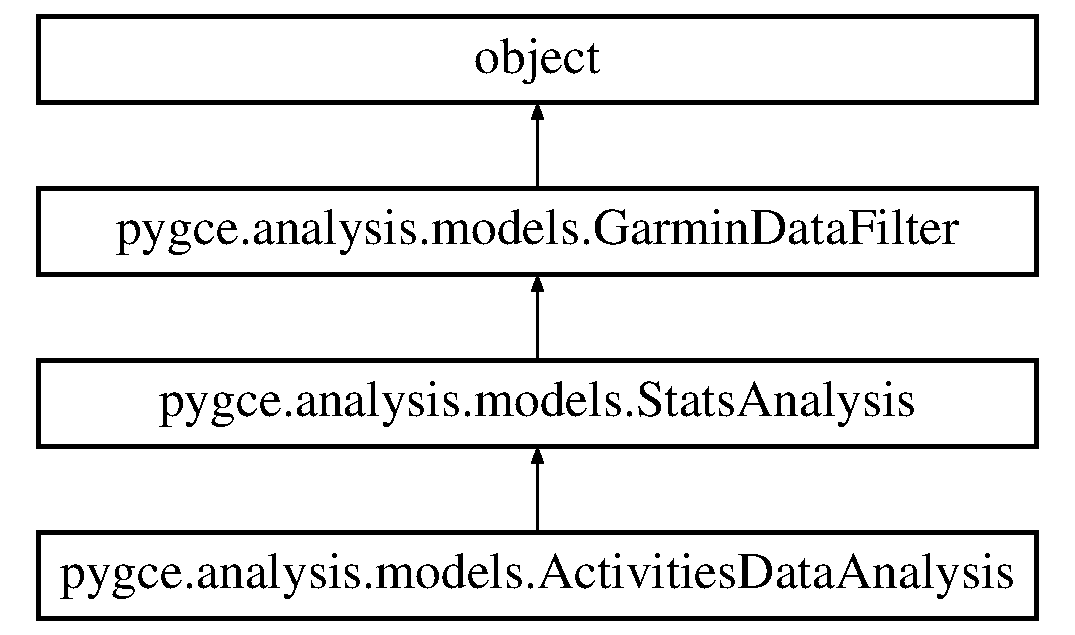
\includegraphics[height=4.000000cm]{classpygce_1_1analysis_1_1models_1_1_activities_data_analysis}
\end{center}
\end{figure}
\subsection*{Public Member Functions}
\begin{DoxyCompactItemize}
\item 
def \hyperlink{classpygce_1_1analysis_1_1models_1_1_activities_data_analysis_a6196617473672f614453a357bcb09799}{\+\_\+\+\_\+init\+\_\+\+\_\+} (self, \hyperlink{classpygce_1_1analysis_1_1models_1_1_garmin_data_filter_a7bb7be05577c2d31546e27823a5d11c5}{dataset\+\_\+file})
\item 
def \hyperlink{classpygce_1_1analysis_1_1models_1_1_activities_data_analysis_a5b3ad1747c5ff3a8cd868ebf8e5724ae}{parse\+\_\+csv} (self)
\item 
def \hyperlink{classpygce_1_1analysis_1_1models_1_1_activities_data_analysis_a7aac6979906baac1801dc83b5ea40360}{shows\+\_\+correlation\+\_\+matrix\+\_\+of\+\_\+data} (self)
\end{DoxyCompactItemize}
\subsection*{Static Public Attributes}
\begin{DoxyCompactItemize}
\item 
list \hyperlink{classpygce_1_1analysis_1_1models_1_1_activities_data_analysis_a799ad90125cc686b985fe525a3b33062}{H\+E\+A\+D\+E\+R\+S\+\_\+\+T\+O\+\_\+\+A\+N\+A\+L\+Y\+ZE}
\item 
list \hyperlink{classpygce_1_1analysis_1_1models_1_1_activities_data_analysis_a2f0ccc7899b8c6b6d94391c80f5def1d}{T\+I\+M\+E\+\_\+\+H\+E\+A\+D\+E\+R\+S\+\_\+\+T\+O\+\_\+\+C\+O\+N\+V\+E\+RT}
\item 
list \hyperlink{classpygce_1_1analysis_1_1models_1_1_activities_data_analysis_a272e010f956a64a8f916ebf1b9e14255}{H\+E\+A\+D\+E\+R\+S\+\_\+\+W\+I\+T\+H\+\_\+\+M\+A\+L\+F\+O\+R\+M\+E\+D\+\_\+\+F\+L\+O\+A\+TS}
\end{DoxyCompactItemize}
\subsection*{Additional Inherited Members}


\subsection{Detailed Description}
\begin{DoxyVerb}Machine-learn activities data \end{DoxyVerb}
 

Definition at line 243 of file models.\+py.



\subsection{Constructor \& Destructor Documentation}
\index{pygce\+::analysis\+::models\+::\+Activities\+Data\+Analysis@{pygce\+::analysis\+::models\+::\+Activities\+Data\+Analysis}!\+\_\+\+\_\+init\+\_\+\+\_\+@{\+\_\+\+\_\+init\+\_\+\+\_\+}}
\index{\+\_\+\+\_\+init\+\_\+\+\_\+@{\+\_\+\+\_\+init\+\_\+\+\_\+}!pygce\+::analysis\+::models\+::\+Activities\+Data\+Analysis@{pygce\+::analysis\+::models\+::\+Activities\+Data\+Analysis}}
\subsubsection[{\texorpdfstring{\+\_\+\+\_\+init\+\_\+\+\_\+(self, dataset\+\_\+file)}{__init__(self, dataset_file)}}]{\setlength{\rightskip}{0pt plus 5cm}def pygce.\+analysis.\+models.\+Activities\+Data\+Analysis.\+\_\+\+\_\+init\+\_\+\+\_\+ (
\begin{DoxyParamCaption}
\item[{}]{self, }
\item[{}]{dataset\+\_\+file}
\end{DoxyParamCaption}
)}\hypertarget{classpygce_1_1analysis_1_1models_1_1_activities_data_analysis_a6196617473672f614453a357bcb09799}{}\label{classpygce_1_1analysis_1_1models_1_1_activities_data_analysis_a6196617473672f614453a357bcb09799}
\begin{DoxyVerb}:param dataset_file: str
    Path to folder with data to analyse
\end{DoxyVerb}
 

Definition at line 269 of file models.\+py.



\subsection{Member Function Documentation}
\index{pygce\+::analysis\+::models\+::\+Activities\+Data\+Analysis@{pygce\+::analysis\+::models\+::\+Activities\+Data\+Analysis}!parse\+\_\+csv@{parse\+\_\+csv}}
\index{parse\+\_\+csv@{parse\+\_\+csv}!pygce\+::analysis\+::models\+::\+Activities\+Data\+Analysis@{pygce\+::analysis\+::models\+::\+Activities\+Data\+Analysis}}
\subsubsection[{\texorpdfstring{parse\+\_\+csv(self)}{parse_csv(self)}}]{\setlength{\rightskip}{0pt plus 5cm}def pygce.\+analysis.\+models.\+Activities\+Data\+Analysis.\+parse\+\_\+csv (
\begin{DoxyParamCaption}
\item[{}]{self}
\end{DoxyParamCaption}
)}\hypertarget{classpygce_1_1analysis_1_1models_1_1_activities_data_analysis_a5b3ad1747c5ff3a8cd868ebf8e5724ae}{}\label{classpygce_1_1analysis_1_1models_1_1_activities_data_analysis_a5b3ad1747c5ff3a8cd868ebf8e5724ae}
\begin{DoxyVerb}:return: tuple [], [] of []
    Headers of csv file and data
\end{DoxyVerb}
 

Definition at line 277 of file models.\+py.

\index{pygce\+::analysis\+::models\+::\+Activities\+Data\+Analysis@{pygce\+::analysis\+::models\+::\+Activities\+Data\+Analysis}!shows\+\_\+correlation\+\_\+matrix\+\_\+of\+\_\+data@{shows\+\_\+correlation\+\_\+matrix\+\_\+of\+\_\+data}}
\index{shows\+\_\+correlation\+\_\+matrix\+\_\+of\+\_\+data@{shows\+\_\+correlation\+\_\+matrix\+\_\+of\+\_\+data}!pygce\+::analysis\+::models\+::\+Activities\+Data\+Analysis@{pygce\+::analysis\+::models\+::\+Activities\+Data\+Analysis}}
\subsubsection[{\texorpdfstring{shows\+\_\+correlation\+\_\+matrix\+\_\+of\+\_\+data(self)}{shows_correlation_matrix_of_data(self)}}]{\setlength{\rightskip}{0pt plus 5cm}def pygce.\+analysis.\+models.\+Activities\+Data\+Analysis.\+shows\+\_\+correlation\+\_\+matrix\+\_\+of\+\_\+data (
\begin{DoxyParamCaption}
\item[{}]{self}
\end{DoxyParamCaption}
)}\hypertarget{classpygce_1_1analysis_1_1models_1_1_activities_data_analysis_a7aac6979906baac1801dc83b5ea40360}{}\label{classpygce_1_1analysis_1_1models_1_1_activities_data_analysis_a7aac6979906baac1801dc83b5ea40360}
\begin{DoxyVerb}:return: void
    Shows correlation matrix of data of files in folder
\end{DoxyVerb}
 

Definition at line 288 of file models.\+py.



\subsection{Member Data Documentation}
\index{pygce\+::analysis\+::models\+::\+Activities\+Data\+Analysis@{pygce\+::analysis\+::models\+::\+Activities\+Data\+Analysis}!H\+E\+A\+D\+E\+R\+S\+\_\+\+T\+O\+\_\+\+A\+N\+A\+L\+Y\+ZE@{H\+E\+A\+D\+E\+R\+S\+\_\+\+T\+O\+\_\+\+A\+N\+A\+L\+Y\+ZE}}
\index{H\+E\+A\+D\+E\+R\+S\+\_\+\+T\+O\+\_\+\+A\+N\+A\+L\+Y\+ZE@{H\+E\+A\+D\+E\+R\+S\+\_\+\+T\+O\+\_\+\+A\+N\+A\+L\+Y\+ZE}!pygce\+::analysis\+::models\+::\+Activities\+Data\+Analysis@{pygce\+::analysis\+::models\+::\+Activities\+Data\+Analysis}}
\subsubsection[{\texorpdfstring{H\+E\+A\+D\+E\+R\+S\+\_\+\+T\+O\+\_\+\+A\+N\+A\+L\+Y\+ZE}{HEADERS_TO_ANALYZE}}]{\setlength{\rightskip}{0pt plus 5cm}list pygce.\+analysis.\+models.\+Activities\+Data\+Analysis.\+H\+E\+A\+D\+E\+R\+S\+\_\+\+T\+O\+\_\+\+A\+N\+A\+L\+Y\+ZE\hspace{0.3cm}{\ttfamily [static]}}\hypertarget{classpygce_1_1analysis_1_1models_1_1_activities_data_analysis_a799ad90125cc686b985fe525a3b33062}{}\label{classpygce_1_1analysis_1_1models_1_1_activities_data_analysis_a799ad90125cc686b985fe525a3b33062}
{\bfseries Initial value\+:}
\begin{DoxyCode}
1 = [
2         \textcolor{stringliteral}{"Distance"},
3         \textcolor{stringliteral}{"Time"},
4         \textcolor{stringliteral}{"Avg Speed(Avg Pace)"},
5         \textcolor{stringliteral}{"Max Speed(Best Pace)"},
6         \textcolor{stringliteral}{"Elevation Gain"},
7         \textcolor{stringliteral}{"Avg HR"},
8         \textcolor{stringliteral}{"Max HR"},
9         \textcolor{stringliteral}{"Avg Run Cadence"},
10         \textcolor{stringliteral}{"Max Run Cadence"},
11         \textcolor{stringliteral}{"Calories"},
12         \textcolor{stringliteral}{"Training Effect"}
13     ]
\end{DoxyCode}


Definition at line 246 of file models.\+py.

\index{pygce\+::analysis\+::models\+::\+Activities\+Data\+Analysis@{pygce\+::analysis\+::models\+::\+Activities\+Data\+Analysis}!H\+E\+A\+D\+E\+R\+S\+\_\+\+W\+I\+T\+H\+\_\+\+M\+A\+L\+F\+O\+R\+M\+E\+D\+\_\+\+F\+L\+O\+A\+TS@{H\+E\+A\+D\+E\+R\+S\+\_\+\+W\+I\+T\+H\+\_\+\+M\+A\+L\+F\+O\+R\+M\+E\+D\+\_\+\+F\+L\+O\+A\+TS}}
\index{H\+E\+A\+D\+E\+R\+S\+\_\+\+W\+I\+T\+H\+\_\+\+M\+A\+L\+F\+O\+R\+M\+E\+D\+\_\+\+F\+L\+O\+A\+TS@{H\+E\+A\+D\+E\+R\+S\+\_\+\+W\+I\+T\+H\+\_\+\+M\+A\+L\+F\+O\+R\+M\+E\+D\+\_\+\+F\+L\+O\+A\+TS}!pygce\+::analysis\+::models\+::\+Activities\+Data\+Analysis@{pygce\+::analysis\+::models\+::\+Activities\+Data\+Analysis}}
\subsubsection[{\texorpdfstring{H\+E\+A\+D\+E\+R\+S\+\_\+\+W\+I\+T\+H\+\_\+\+M\+A\+L\+F\+O\+R\+M\+E\+D\+\_\+\+F\+L\+O\+A\+TS}{HEADERS_WITH_MALFORMED_FLOATS}}]{\setlength{\rightskip}{0pt plus 5cm}list pygce.\+analysis.\+models.\+Activities\+Data\+Analysis.\+H\+E\+A\+D\+E\+R\+S\+\_\+\+W\+I\+T\+H\+\_\+\+M\+A\+L\+F\+O\+R\+M\+E\+D\+\_\+\+F\+L\+O\+A\+TS\hspace{0.3cm}{\ttfamily [static]}}\hypertarget{classpygce_1_1analysis_1_1models_1_1_activities_data_analysis_a272e010f956a64a8f916ebf1b9e14255}{}\label{classpygce_1_1analysis_1_1models_1_1_activities_data_analysis_a272e010f956a64a8f916ebf1b9e14255}
{\bfseries Initial value\+:}
\begin{DoxyCode}
1 = [
2         \textcolor{stringliteral}{"Distance"},
3         \textcolor{stringliteral}{"Training Effect"}
4     ]
\end{DoxyCode}


Definition at line 264 of file models.\+py.

\index{pygce\+::analysis\+::models\+::\+Activities\+Data\+Analysis@{pygce\+::analysis\+::models\+::\+Activities\+Data\+Analysis}!T\+I\+M\+E\+\_\+\+H\+E\+A\+D\+E\+R\+S\+\_\+\+T\+O\+\_\+\+C\+O\+N\+V\+E\+RT@{T\+I\+M\+E\+\_\+\+H\+E\+A\+D\+E\+R\+S\+\_\+\+T\+O\+\_\+\+C\+O\+N\+V\+E\+RT}}
\index{T\+I\+M\+E\+\_\+\+H\+E\+A\+D\+E\+R\+S\+\_\+\+T\+O\+\_\+\+C\+O\+N\+V\+E\+RT@{T\+I\+M\+E\+\_\+\+H\+E\+A\+D\+E\+R\+S\+\_\+\+T\+O\+\_\+\+C\+O\+N\+V\+E\+RT}!pygce\+::analysis\+::models\+::\+Activities\+Data\+Analysis@{pygce\+::analysis\+::models\+::\+Activities\+Data\+Analysis}}
\subsubsection[{\texorpdfstring{T\+I\+M\+E\+\_\+\+H\+E\+A\+D\+E\+R\+S\+\_\+\+T\+O\+\_\+\+C\+O\+N\+V\+E\+RT}{TIME_HEADERS_TO_CONVERT}}]{\setlength{\rightskip}{0pt plus 5cm}list pygce.\+analysis.\+models.\+Activities\+Data\+Analysis.\+T\+I\+M\+E\+\_\+\+H\+E\+A\+D\+E\+R\+S\+\_\+\+T\+O\+\_\+\+C\+O\+N\+V\+E\+RT\hspace{0.3cm}{\ttfamily [static]}}\hypertarget{classpygce_1_1analysis_1_1models_1_1_activities_data_analysis_a2f0ccc7899b8c6b6d94391c80f5def1d}{}\label{classpygce_1_1analysis_1_1models_1_1_activities_data_analysis_a2f0ccc7899b8c6b6d94391c80f5def1d}
{\bfseries Initial value\+:}
\begin{DoxyCode}
1 = [
2         \textcolor{stringliteral}{"Time"},
3         \textcolor{stringliteral}{"Avg Speed(Avg Pace)"},
4         \textcolor{stringliteral}{"Max Speed(Best Pace)"}
5     ]
\end{DoxyCode}


Definition at line 259 of file models.\+py.



The documentation for this class was generated from the following file\+:\begin{DoxyCompactItemize}
\item 
/home/stefano/\+Coding/\+Python/projects/garmin-\/connect-\/export/pygce/analysis/\hyperlink{models_8py}{models.\+py}\end{DoxyCompactItemize}

\hypertarget{classpygce_1_1models_1_1bot_1_1_garmin_connect_bot}{}\section{pygce.\+models.\+bot.\+Garmin\+Connect\+Bot Class Reference}
\label{classpygce_1_1models_1_1bot_1_1_garmin_connect_bot}\index{pygce.\+models.\+bot.\+Garmin\+Connect\+Bot@{pygce.\+models.\+bot.\+Garmin\+Connect\+Bot}}
Inheritance diagram for pygce.\+models.\+bot.\+Garmin\+Connect\+Bot\+:\begin{figure}[H]
\begin{center}
\leavevmode
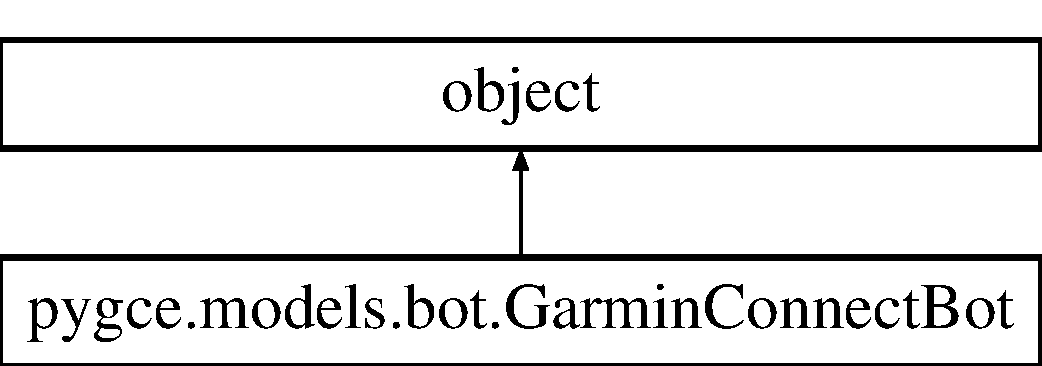
\includegraphics[height=2.000000cm]{classpygce_1_1models_1_1bot_1_1_garmin_connect_bot}
\end{center}
\end{figure}
\subsection*{Public Member Functions}
\begin{DoxyCompactItemize}
\item 
def \hyperlink{classpygce_1_1models_1_1bot_1_1_garmin_connect_bot_aeb909c53e6a647b5e8419d4877ba5b6d}{\+\_\+\+\_\+init\+\_\+\+\_\+} (self, \hyperlink{classpygce_1_1models_1_1bot_1_1_garmin_connect_bot_a259da08c172fe9b54bbb6b997ab840a7}{user\+\_\+name}, password, \hyperlink{classpygce_1_1models_1_1bot_1_1_garmin_connect_bot_a81b2ce5ff74592aeb9b1d8ebc236bfe4}{download\+\_\+gpx}, chromedriver\+\_\+path, url=\hyperlink{classpygce_1_1models_1_1bot_1_1_garmin_connect_bot_a860621296516b8e3793321d0773e30f3}{D\+E\+F\+A\+U\+L\+T\+\_\+\+B\+A\+S\+E\+\_\+\+U\+RL})
\item 
def \hyperlink{classpygce_1_1models_1_1bot_1_1_garmin_connect_bot_a31c8153cff1e4c2ce2a66d3b3aada3f1}{login} (self)
\item 
def \hyperlink{classpygce_1_1models_1_1bot_1_1_garmin_connect_bot_ad9433580f9aced25b650ddd5e912cc52}{go\+\_\+to\+\_\+dashboard} (self)
\item 
def \hyperlink{classpygce_1_1models_1_1bot_1_1_garmin_connect_bot_a3a0df451b2e7c0667064adc5c0ba1ad5}{go\+\_\+to\+\_\+day} (self, date\+\_\+time)
\item 
def \hyperlink{classpygce_1_1models_1_1bot_1_1_garmin_connect_bot_ab5ab1e855230273b7c7c085a461a3ed2}{get\+\_\+day} (self, date\+\_\+time)
\item 
def \hyperlink{classpygce_1_1models_1_1bot_1_1_garmin_connect_bot_a18ab2d80266a9da67186bcba6b4856b9}{get\+\_\+days} (self, min\+\_\+date\+\_\+time, max\+\_\+date\+\_\+time)
\item 
def \hyperlink{classpygce_1_1models_1_1bot_1_1_garmin_connect_bot_a17c3b23e3a712395581e88294308b822}{parse\+\_\+days} (self, min\+\_\+date\+\_\+time, max\+\_\+date\+\_\+time)
\item 
def \hyperlink{classpygce_1_1models_1_1bot_1_1_garmin_connect_bot_a6b7760e4013e2ada06bed1a5f47133f1}{save\+\_\+json\+\_\+days} (self, min\+\_\+date\+\_\+time, max\+\_\+date\+\_\+time, output\+\_\+file)
\item 
def \hyperlink{classpygce_1_1models_1_1bot_1_1_garmin_connect_bot_ac10284acc765724afd060381ace0cb5e}{save\+\_\+csv\+\_\+days} (self, min\+\_\+date\+\_\+time, max\+\_\+date\+\_\+time, output\+\_\+file)
\item 
def \hyperlink{classpygce_1_1models_1_1bot_1_1_garmin_connect_bot_a9cd831d6a4a8efdd793a395f99fc1796}{save\+\_\+gpx} (self, data)
\end{DoxyCompactItemize}
\subsection*{Public Attributes}
\begin{DoxyCompactItemize}
\item 
\hyperlink{classpygce_1_1models_1_1bot_1_1_garmin_connect_bot_a60f14c87e68f9067680ba264205a0f5c}{browser}
\item 
\hyperlink{classpygce_1_1models_1_1bot_1_1_garmin_connect_bot_a259da08c172fe9b54bbb6b997ab840a7}{user\+\_\+name}
\item 
\hyperlink{classpygce_1_1models_1_1bot_1_1_garmin_connect_bot_af3d5c76d7e90a6aefe67926755d08c01}{user\+\_\+password}
\item 
\hyperlink{classpygce_1_1models_1_1bot_1_1_garmin_connect_bot_ae6d646cac47d9930a50be37aad133dea}{user\+\_\+logged\+\_\+in}
\item 
\hyperlink{classpygce_1_1models_1_1bot_1_1_garmin_connect_bot_a762d018855af5616f0519e08c354a7c7}{user\+\_\+id}
\item 
\hyperlink{classpygce_1_1models_1_1bot_1_1_garmin_connect_bot_a81b2ce5ff74592aeb9b1d8ebc236bfe4}{download\+\_\+gpx}
\item 
\hyperlink{classpygce_1_1models_1_1bot_1_1_garmin_connect_bot_a6afbf3f00e551c7a29de3b18e86f1eb2}{user\+\_\+url}
\item 
\hyperlink{classpygce_1_1models_1_1bot_1_1_garmin_connect_bot_a4ae874d8c53c9e6ff04fb7d72ba54f52}{base\+\_\+url}
\item 
\hyperlink{classpygce_1_1models_1_1bot_1_1_garmin_connect_bot_a9ae225cd44515fe8675b123b1907492e}{login\+\_\+url}
\end{DoxyCompactItemize}
\subsection*{Static Public Attributes}
\begin{DoxyCompactItemize}
\item 
string \hyperlink{classpygce_1_1models_1_1bot_1_1_garmin_connect_bot_aa0d174bafc498e1c037324e16fd0dbe0}{U\+S\+E\+R\+\_\+\+P\+A\+TH} = \char`\"{}/modern/\char`\"{}
\item 
string \hyperlink{classpygce_1_1models_1_1bot_1_1_garmin_connect_bot_a860621296516b8e3793321d0773e30f3}{D\+E\+F\+A\+U\+L\+T\+\_\+\+B\+A\+S\+E\+\_\+\+U\+RL} = \char`\"{}https\+://connect.\+garmin.\+com\char`\"{}
\item 
string \hyperlink{classpygce_1_1models_1_1bot_1_1_garmin_connect_bot_aad154f2121928191c68ac2f9530470e3}{B\+A\+S\+E\+\_\+\+L\+O\+G\+I\+N\+\_\+\+U\+RL} = \char`\"{}https\+://sso.\+garmin.\+com/sso/\hyperlink{classpygce_1_1models_1_1bot_1_1_garmin_connect_bot_a31c8153cff1e4c2ce2a66d3b3aada3f1}{login}?service=https\%3\+A\%2\+F\char`\"{} \textbackslash{}
\item 
string \hyperlink{classpygce_1_1models_1_1bot_1_1_garmin_connect_bot_a792c3468032c4154b334cacfb30a871f}{L\+O\+G\+I\+N\+\_\+\+B\+U\+T\+T\+O\+N\+\_\+\+ID} = \char`\"{}login-\/btn-\/signin\char`\"{}
\item 
string \hyperlink{classpygce_1_1models_1_1bot_1_1_garmin_connect_bot_a0128de4e9df3cd9171f697709b634865}{U\+S\+E\+R\+N\+A\+M\+E\+\_\+\+F\+I\+E\+L\+D\+\_\+\+N\+A\+ME} = \char`\"{}username\char`\"{}
\item 
string \hyperlink{classpygce_1_1models_1_1bot_1_1_garmin_connect_bot_aa5839cf18d60997c81245cebea3eb307}{P\+A\+S\+S\+W\+O\+R\+D\+\_\+\+F\+I\+E\+L\+D\+\_\+\+N\+A\+ME} = \char`\"{}password\char`\"{}
\item 
int \hyperlink{classpygce_1_1models_1_1bot_1_1_garmin_connect_bot_a71d72a5424537d2a39e05e75f654697e}{B\+R\+O\+W\+S\+E\+R\+\_\+\+W\+A\+I\+T\+\_\+\+T\+I\+M\+E\+O\+U\+T\+\_\+\+S\+E\+C\+O\+N\+DS} = 3
\item 
string \hyperlink{classpygce_1_1models_1_1bot_1_1_garmin_connect_bot_afb55db5c02bec7ec7493dacdd65b31d7}{B\+R\+O\+W\+S\+E\+R\+\_\+\+G\+E\+N\+E\+R\+A\+L\+\_\+\+E\+R\+R\+OR} = \char`\"{}If the error persist, please open an issue.\char`\"{}
\item 
string \hyperlink{classpygce_1_1models_1_1bot_1_1_garmin_connect_bot_ad2a1e0946d0f6325bb4fdd8564fe7665}{B\+R\+O\+W\+S\+E\+R\+\_\+\+T\+I\+M\+E\+O\+U\+T\+\_\+\+E\+R\+R\+OR} = \char`\"{}Cannot complete request (cannot find \{\}). I \char`\"{} \textbackslash{}
\end{DoxyCompactItemize}


\subsection{Detailed Description}
\begin{DoxyVerb}Navigate through Garmin Connect app via a bot \end{DoxyVerb}
 

Definition at line 20 of file bot.\+py.



\subsection{Constructor \& Destructor Documentation}
\mbox{\Hypertarget{classpygce_1_1models_1_1bot_1_1_garmin_connect_bot_aeb909c53e6a647b5e8419d4877ba5b6d}\label{classpygce_1_1models_1_1bot_1_1_garmin_connect_bot_aeb909c53e6a647b5e8419d4877ba5b6d}} 
\index{pygce\+::models\+::bot\+::\+Garmin\+Connect\+Bot@{pygce\+::models\+::bot\+::\+Garmin\+Connect\+Bot}!\+\_\+\+\_\+init\+\_\+\+\_\+@{\+\_\+\+\_\+init\+\_\+\+\_\+}}
\index{\+\_\+\+\_\+init\+\_\+\+\_\+@{\+\_\+\+\_\+init\+\_\+\+\_\+}!pygce\+::models\+::bot\+::\+Garmin\+Connect\+Bot@{pygce\+::models\+::bot\+::\+Garmin\+Connect\+Bot}}
\subsubsection{\texorpdfstring{\+\_\+\+\_\+init\+\_\+\+\_\+()}{\_\_init\_\_()}}
{\footnotesize\ttfamily def pygce.\+models.\+bot.\+Garmin\+Connect\+Bot.\+\_\+\+\_\+init\+\_\+\+\_\+ (\begin{DoxyParamCaption}\item[{}]{self,  }\item[{}]{user\+\_\+name,  }\item[{}]{password,  }\item[{}]{download\+\_\+gpx,  }\item[{}]{chromedriver\+\_\+path,  }\item[{}]{url = {\ttfamily \hyperlink{classpygce_1_1models_1_1bot_1_1_garmin_connect_bot_a860621296516b8e3793321d0773e30f3}{D\+E\+F\+A\+U\+L\+T\+\_\+\+B\+A\+S\+E\+\_\+\+U\+RL}} }\end{DoxyParamCaption})}

\begin{DoxyVerb}:param user_name: str
    Username (email) to login to Garmin Connect
:param password: str
    Password to login to Garmin Connect
:param download_gpx: bool
    Download .gpx files of activities
:param chromedriver_path: str
    Path to Chrome driver to use as browser
:param url: str
    Url to base downloads on
\end{DoxyVerb}
 

Definition at line 43 of file bot.\+py.



\subsection{Member Function Documentation}
\mbox{\Hypertarget{classpygce_1_1models_1_1bot_1_1_garmin_connect_bot_ab5ab1e855230273b7c7c085a461a3ed2}\label{classpygce_1_1models_1_1bot_1_1_garmin_connect_bot_ab5ab1e855230273b7c7c085a461a3ed2}} 
\index{pygce\+::models\+::bot\+::\+Garmin\+Connect\+Bot@{pygce\+::models\+::bot\+::\+Garmin\+Connect\+Bot}!get\+\_\+day@{get\+\_\+day}}
\index{get\+\_\+day@{get\+\_\+day}!pygce\+::models\+::bot\+::\+Garmin\+Connect\+Bot@{pygce\+::models\+::bot\+::\+Garmin\+Connect\+Bot}}
\subsubsection{\texorpdfstring{get\+\_\+day()}{get\_day()}}
{\footnotesize\ttfamily def pygce.\+models.\+bot.\+Garmin\+Connect\+Bot.\+get\+\_\+day (\begin{DoxyParamCaption}\item[{}]{self,  }\item[{}]{date\+\_\+time }\end{DoxyParamCaption})}

\begin{DoxyVerb}:param date_time: datetime
    Datetime object with date
:return: GCDayTimline
    Data about day
\end{DoxyVerb}
 

Definition at line 181 of file bot.\+py.

\mbox{\Hypertarget{classpygce_1_1models_1_1bot_1_1_garmin_connect_bot_a18ab2d80266a9da67186bcba6b4856b9}\label{classpygce_1_1models_1_1bot_1_1_garmin_connect_bot_a18ab2d80266a9da67186bcba6b4856b9}} 
\index{pygce\+::models\+::bot\+::\+Garmin\+Connect\+Bot@{pygce\+::models\+::bot\+::\+Garmin\+Connect\+Bot}!get\+\_\+days@{get\+\_\+days}}
\index{get\+\_\+days@{get\+\_\+days}!pygce\+::models\+::bot\+::\+Garmin\+Connect\+Bot@{pygce\+::models\+::bot\+::\+Garmin\+Connect\+Bot}}
\subsubsection{\texorpdfstring{get\+\_\+days()}{get\_days()}}
{\footnotesize\ttfamily def pygce.\+models.\+bot.\+Garmin\+Connect\+Bot.\+get\+\_\+days (\begin{DoxyParamCaption}\item[{}]{self,  }\item[{}]{min\+\_\+date\+\_\+time,  }\item[{}]{max\+\_\+date\+\_\+time }\end{DoxyParamCaption})}

\begin{DoxyVerb}:param min_date_time: datetime
    Datetime object with date, this is the date when to start downloading data
:param max_date_time: datetime
    Datetime object with date, this is the date when to stop downloading data
:return: [] of GCDayTimline
    List of data about days
\end{DoxyVerb}
 

Definition at line 231 of file bot.\+py.

\mbox{\Hypertarget{classpygce_1_1models_1_1bot_1_1_garmin_connect_bot_ad9433580f9aced25b650ddd5e912cc52}\label{classpygce_1_1models_1_1bot_1_1_garmin_connect_bot_ad9433580f9aced25b650ddd5e912cc52}} 
\index{pygce\+::models\+::bot\+::\+Garmin\+Connect\+Bot@{pygce\+::models\+::bot\+::\+Garmin\+Connect\+Bot}!go\+\_\+to\+\_\+dashboard@{go\+\_\+to\+\_\+dashboard}}
\index{go\+\_\+to\+\_\+dashboard@{go\+\_\+to\+\_\+dashboard}!pygce\+::models\+::bot\+::\+Garmin\+Connect\+Bot@{pygce\+::models\+::bot\+::\+Garmin\+Connect\+Bot}}
\subsubsection{\texorpdfstring{go\+\_\+to\+\_\+dashboard()}{go\_to\_dashboard()}}
{\footnotesize\ttfamily def pygce.\+models.\+bot.\+Garmin\+Connect\+Bot.\+go\+\_\+to\+\_\+dashboard (\begin{DoxyParamCaption}\item[{}]{self }\end{DoxyParamCaption})}

\begin{DoxyVerb}:return: void
    Navigates to user homepage
\end{DoxyVerb}
 

Definition at line 153 of file bot.\+py.

\mbox{\Hypertarget{classpygce_1_1models_1_1bot_1_1_garmin_connect_bot_a3a0df451b2e7c0667064adc5c0ba1ad5}\label{classpygce_1_1models_1_1bot_1_1_garmin_connect_bot_a3a0df451b2e7c0667064adc5c0ba1ad5}} 
\index{pygce\+::models\+::bot\+::\+Garmin\+Connect\+Bot@{pygce\+::models\+::bot\+::\+Garmin\+Connect\+Bot}!go\+\_\+to\+\_\+day@{go\+\_\+to\+\_\+day}}
\index{go\+\_\+to\+\_\+day@{go\+\_\+to\+\_\+day}!pygce\+::models\+::bot\+::\+Garmin\+Connect\+Bot@{pygce\+::models\+::bot\+::\+Garmin\+Connect\+Bot}}
\subsubsection{\texorpdfstring{go\+\_\+to\+\_\+day()}{go\_to\_day()}}
{\footnotesize\ttfamily def pygce.\+models.\+bot.\+Garmin\+Connect\+Bot.\+go\+\_\+to\+\_\+day (\begin{DoxyParamCaption}\item[{}]{self,  }\item[{}]{date\+\_\+time }\end{DoxyParamCaption})}

\begin{DoxyVerb}:param date_time: datetime
    Datetime object with date
:return: void
    Navigates to daily summary of given date
\end{DoxyVerb}
 

Definition at line 169 of file bot.\+py.

\mbox{\Hypertarget{classpygce_1_1models_1_1bot_1_1_garmin_connect_bot_a31c8153cff1e4c2ce2a66d3b3aada3f1}\label{classpygce_1_1models_1_1bot_1_1_garmin_connect_bot_a31c8153cff1e4c2ce2a66d3b3aada3f1}} 
\index{pygce\+::models\+::bot\+::\+Garmin\+Connect\+Bot@{pygce\+::models\+::bot\+::\+Garmin\+Connect\+Bot}!login@{login}}
\index{login@{login}!pygce\+::models\+::bot\+::\+Garmin\+Connect\+Bot@{pygce\+::models\+::bot\+::\+Garmin\+Connect\+Bot}}
\subsubsection{\texorpdfstring{login()}{login()}}
{\footnotesize\ttfamily def pygce.\+models.\+bot.\+Garmin\+Connect\+Bot.\+login (\begin{DoxyParamCaption}\item[{}]{self }\end{DoxyParamCaption})}

\begin{DoxyVerb}:return: bool
    True iff correctly logged in
\end{DoxyVerb}
 

Definition at line 112 of file bot.\+py.

\mbox{\Hypertarget{classpygce_1_1models_1_1bot_1_1_garmin_connect_bot_a17c3b23e3a712395581e88294308b822}\label{classpygce_1_1models_1_1bot_1_1_garmin_connect_bot_a17c3b23e3a712395581e88294308b822}} 
\index{pygce\+::models\+::bot\+::\+Garmin\+Connect\+Bot@{pygce\+::models\+::bot\+::\+Garmin\+Connect\+Bot}!parse\+\_\+days@{parse\+\_\+days}}
\index{parse\+\_\+days@{parse\+\_\+days}!pygce\+::models\+::bot\+::\+Garmin\+Connect\+Bot@{pygce\+::models\+::bot\+::\+Garmin\+Connect\+Bot}}
\subsubsection{\texorpdfstring{parse\+\_\+days()}{parse\_days()}}
{\footnotesize\ttfamily def pygce.\+models.\+bot.\+Garmin\+Connect\+Bot.\+parse\+\_\+days (\begin{DoxyParamCaption}\item[{}]{self,  }\item[{}]{min\+\_\+date\+\_\+time,  }\item[{}]{max\+\_\+date\+\_\+time }\end{DoxyParamCaption})}

\begin{DoxyVerb}:param min_date_time: datetime
    Datetime object with date, this is the date when to start downloading data
:param max_date_time: datetime
    Datetime object with date, this is the date when to stop downloading data
:return: []
    List of data about days
\end{DoxyVerb}
 

Definition at line 252 of file bot.\+py.

\mbox{\Hypertarget{classpygce_1_1models_1_1bot_1_1_garmin_connect_bot_ac10284acc765724afd060381ace0cb5e}\label{classpygce_1_1models_1_1bot_1_1_garmin_connect_bot_ac10284acc765724afd060381ace0cb5e}} 
\index{pygce\+::models\+::bot\+::\+Garmin\+Connect\+Bot@{pygce\+::models\+::bot\+::\+Garmin\+Connect\+Bot}!save\+\_\+csv\+\_\+days@{save\+\_\+csv\+\_\+days}}
\index{save\+\_\+csv\+\_\+days@{save\+\_\+csv\+\_\+days}!pygce\+::models\+::bot\+::\+Garmin\+Connect\+Bot@{pygce\+::models\+::bot\+::\+Garmin\+Connect\+Bot}}
\subsubsection{\texorpdfstring{save\+\_\+csv\+\_\+days()}{save\_csv\_days()}}
{\footnotesize\ttfamily def pygce.\+models.\+bot.\+Garmin\+Connect\+Bot.\+save\+\_\+csv\+\_\+days (\begin{DoxyParamCaption}\item[{}]{self,  }\item[{}]{min\+\_\+date\+\_\+time,  }\item[{}]{max\+\_\+date\+\_\+time,  }\item[{}]{output\+\_\+file }\end{DoxyParamCaption})}

\begin{DoxyVerb}:param min_date_time: datetime
    Datetime object with date, this is the date when to start downloading data
:param max_date_time: datetime
    Datetime object with date, this is the date when to stop downloading data
:param output_file: str
    Path where to save output to
:return: void
    Retrieves data about days in given range, then saves csv dump
\end{DoxyVerb}
 

Definition at line 291 of file bot.\+py.

\mbox{\Hypertarget{classpygce_1_1models_1_1bot_1_1_garmin_connect_bot_a9cd831d6a4a8efdd793a395f99fc1796}\label{classpygce_1_1models_1_1bot_1_1_garmin_connect_bot_a9cd831d6a4a8efdd793a395f99fc1796}} 
\index{pygce\+::models\+::bot\+::\+Garmin\+Connect\+Bot@{pygce\+::models\+::bot\+::\+Garmin\+Connect\+Bot}!save\+\_\+gpx@{save\+\_\+gpx}}
\index{save\+\_\+gpx@{save\+\_\+gpx}!pygce\+::models\+::bot\+::\+Garmin\+Connect\+Bot@{pygce\+::models\+::bot\+::\+Garmin\+Connect\+Bot}}
\subsubsection{\texorpdfstring{save\+\_\+gpx()}{save\_gpx()}}
{\footnotesize\ttfamily def pygce.\+models.\+bot.\+Garmin\+Connect\+Bot.\+save\+\_\+gpx (\begin{DoxyParamCaption}\item[{}]{self,  }\item[{}]{data }\end{DoxyParamCaption})}

\begin{DoxyVerb}:param data: [] of GCDayTimeline
    Timeline with activities
:return: void
    Downloads .gpx file for each activity to folder
\end{DoxyVerb}
 

Definition at line 314 of file bot.\+py.

\mbox{\Hypertarget{classpygce_1_1models_1_1bot_1_1_garmin_connect_bot_a6b7760e4013e2ada06bed1a5f47133f1}\label{classpygce_1_1models_1_1bot_1_1_garmin_connect_bot_a6b7760e4013e2ada06bed1a5f47133f1}} 
\index{pygce\+::models\+::bot\+::\+Garmin\+Connect\+Bot@{pygce\+::models\+::bot\+::\+Garmin\+Connect\+Bot}!save\+\_\+json\+\_\+days@{save\+\_\+json\+\_\+days}}
\index{save\+\_\+json\+\_\+days@{save\+\_\+json\+\_\+days}!pygce\+::models\+::bot\+::\+Garmin\+Connect\+Bot@{pygce\+::models\+::bot\+::\+Garmin\+Connect\+Bot}}
\subsubsection{\texorpdfstring{save\+\_\+json\+\_\+days()}{save\_json\_days()}}
{\footnotesize\ttfamily def pygce.\+models.\+bot.\+Garmin\+Connect\+Bot.\+save\+\_\+json\+\_\+days (\begin{DoxyParamCaption}\item[{}]{self,  }\item[{}]{min\+\_\+date\+\_\+time,  }\item[{}]{max\+\_\+date\+\_\+time,  }\item[{}]{output\+\_\+file }\end{DoxyParamCaption})}

\begin{DoxyVerb}:param min_date_time: datetime
    Datetime object with date, this is the date when to start downloading data
:param max_date_time: datetime
    Datetime object with date, this is the date when to stop downloading data
:param output_file: str
    Path where to save output to
:return: void
    Retrieves data about days in given range, then saves json dump
\end{DoxyVerb}
 

Definition at line 270 of file bot.\+py.



\subsection{Member Data Documentation}
\mbox{\Hypertarget{classpygce_1_1models_1_1bot_1_1_garmin_connect_bot_aad154f2121928191c68ac2f9530470e3}\label{classpygce_1_1models_1_1bot_1_1_garmin_connect_bot_aad154f2121928191c68ac2f9530470e3}} 
\index{pygce\+::models\+::bot\+::\+Garmin\+Connect\+Bot@{pygce\+::models\+::bot\+::\+Garmin\+Connect\+Bot}!B\+A\+S\+E\+\_\+\+L\+O\+G\+I\+N\+\_\+\+U\+RL@{B\+A\+S\+E\+\_\+\+L\+O\+G\+I\+N\+\_\+\+U\+RL}}
\index{B\+A\+S\+E\+\_\+\+L\+O\+G\+I\+N\+\_\+\+U\+RL@{B\+A\+S\+E\+\_\+\+L\+O\+G\+I\+N\+\_\+\+U\+RL}!pygce\+::models\+::bot\+::\+Garmin\+Connect\+Bot@{pygce\+::models\+::bot\+::\+Garmin\+Connect\+Bot}}
\subsubsection{\texorpdfstring{B\+A\+S\+E\+\_\+\+L\+O\+G\+I\+N\+\_\+\+U\+RL}{BASE\_LOGIN\_URL}}
{\footnotesize\ttfamily string pygce.\+models.\+bot.\+Garmin\+Connect\+Bot.\+B\+A\+S\+E\+\_\+\+L\+O\+G\+I\+N\+\_\+\+U\+RL = \char`\"{}https\+://sso.\+garmin.\+com/sso/\hyperlink{classpygce_1_1models_1_1bot_1_1_garmin_connect_bot_a31c8153cff1e4c2ce2a66d3b3aada3f1}{login}?service=https\%3\+A\%2\+F\char`\"{} \textbackslash{}\hspace{0.3cm}{\ttfamily [static]}}



Definition at line 25 of file bot.\+py.

\mbox{\Hypertarget{classpygce_1_1models_1_1bot_1_1_garmin_connect_bot_a4ae874d8c53c9e6ff04fb7d72ba54f52}\label{classpygce_1_1models_1_1bot_1_1_garmin_connect_bot_a4ae874d8c53c9e6ff04fb7d72ba54f52}} 
\index{pygce\+::models\+::bot\+::\+Garmin\+Connect\+Bot@{pygce\+::models\+::bot\+::\+Garmin\+Connect\+Bot}!base\+\_\+url@{base\+\_\+url}}
\index{base\+\_\+url@{base\+\_\+url}!pygce\+::models\+::bot\+::\+Garmin\+Connect\+Bot@{pygce\+::models\+::bot\+::\+Garmin\+Connect\+Bot}}
\subsubsection{\texorpdfstring{base\+\_\+url}{base\_url}}
{\footnotesize\ttfamily pygce.\+models.\+bot.\+Garmin\+Connect\+Bot.\+base\+\_\+url}



Definition at line 67 of file bot.\+py.

\mbox{\Hypertarget{classpygce_1_1models_1_1bot_1_1_garmin_connect_bot_a60f14c87e68f9067680ba264205a0f5c}\label{classpygce_1_1models_1_1bot_1_1_garmin_connect_bot_a60f14c87e68f9067680ba264205a0f5c}} 
\index{pygce\+::models\+::bot\+::\+Garmin\+Connect\+Bot@{pygce\+::models\+::bot\+::\+Garmin\+Connect\+Bot}!browser@{browser}}
\index{browser@{browser}!pygce\+::models\+::bot\+::\+Garmin\+Connect\+Bot@{pygce\+::models\+::bot\+::\+Garmin\+Connect\+Bot}}
\subsubsection{\texorpdfstring{browser}{browser}}
{\footnotesize\ttfamily pygce.\+models.\+bot.\+Garmin\+Connect\+Bot.\+browser}



Definition at line 59 of file bot.\+py.

\mbox{\Hypertarget{classpygce_1_1models_1_1bot_1_1_garmin_connect_bot_afb55db5c02bec7ec7493dacdd65b31d7}\label{classpygce_1_1models_1_1bot_1_1_garmin_connect_bot_afb55db5c02bec7ec7493dacdd65b31d7}} 
\index{pygce\+::models\+::bot\+::\+Garmin\+Connect\+Bot@{pygce\+::models\+::bot\+::\+Garmin\+Connect\+Bot}!B\+R\+O\+W\+S\+E\+R\+\_\+\+G\+E\+N\+E\+R\+A\+L\+\_\+\+E\+R\+R\+OR@{B\+R\+O\+W\+S\+E\+R\+\_\+\+G\+E\+N\+E\+R\+A\+L\+\_\+\+E\+R\+R\+OR}}
\index{B\+R\+O\+W\+S\+E\+R\+\_\+\+G\+E\+N\+E\+R\+A\+L\+\_\+\+E\+R\+R\+OR@{B\+R\+O\+W\+S\+E\+R\+\_\+\+G\+E\+N\+E\+R\+A\+L\+\_\+\+E\+R\+R\+OR}!pygce\+::models\+::bot\+::\+Garmin\+Connect\+Bot@{pygce\+::models\+::bot\+::\+Garmin\+Connect\+Bot}}
\subsubsection{\texorpdfstring{B\+R\+O\+W\+S\+E\+R\+\_\+\+G\+E\+N\+E\+R\+A\+L\+\_\+\+E\+R\+R\+OR}{BROWSER\_GENERAL\_ERROR}}
{\footnotesize\ttfamily string pygce.\+models.\+bot.\+Garmin\+Connect\+Bot.\+B\+R\+O\+W\+S\+E\+R\+\_\+\+G\+E\+N\+E\+R\+A\+L\+\_\+\+E\+R\+R\+OR = \char`\"{}If the error persist, please open an issue.\char`\"{}\hspace{0.3cm}{\ttfamily [static]}}



Definition at line 37 of file bot.\+py.

\mbox{\Hypertarget{classpygce_1_1models_1_1bot_1_1_garmin_connect_bot_ad2a1e0946d0f6325bb4fdd8564fe7665}\label{classpygce_1_1models_1_1bot_1_1_garmin_connect_bot_ad2a1e0946d0f6325bb4fdd8564fe7665}} 
\index{pygce\+::models\+::bot\+::\+Garmin\+Connect\+Bot@{pygce\+::models\+::bot\+::\+Garmin\+Connect\+Bot}!B\+R\+O\+W\+S\+E\+R\+\_\+\+T\+I\+M\+E\+O\+U\+T\+\_\+\+E\+R\+R\+OR@{B\+R\+O\+W\+S\+E\+R\+\_\+\+T\+I\+M\+E\+O\+U\+T\+\_\+\+E\+R\+R\+OR}}
\index{B\+R\+O\+W\+S\+E\+R\+\_\+\+T\+I\+M\+E\+O\+U\+T\+\_\+\+E\+R\+R\+OR@{B\+R\+O\+W\+S\+E\+R\+\_\+\+T\+I\+M\+E\+O\+U\+T\+\_\+\+E\+R\+R\+OR}!pygce\+::models\+::bot\+::\+Garmin\+Connect\+Bot@{pygce\+::models\+::bot\+::\+Garmin\+Connect\+Bot}}
\subsubsection{\texorpdfstring{B\+R\+O\+W\+S\+E\+R\+\_\+\+T\+I\+M\+E\+O\+U\+T\+\_\+\+E\+R\+R\+OR}{BROWSER\_TIMEOUT\_ERROR}}
{\footnotesize\ttfamily string pygce.\+models.\+bot.\+Garmin\+Connect\+Bot.\+B\+R\+O\+W\+S\+E\+R\+\_\+\+T\+I\+M\+E\+O\+U\+T\+\_\+\+E\+R\+R\+OR = \char`\"{}Cannot complete request (cannot find \{\}). I \char`\"{} \textbackslash{}\hspace{0.3cm}{\ttfamily [static]}}



Definition at line 38 of file bot.\+py.

\mbox{\Hypertarget{classpygce_1_1models_1_1bot_1_1_garmin_connect_bot_a71d72a5424537d2a39e05e75f654697e}\label{classpygce_1_1models_1_1bot_1_1_garmin_connect_bot_a71d72a5424537d2a39e05e75f654697e}} 
\index{pygce\+::models\+::bot\+::\+Garmin\+Connect\+Bot@{pygce\+::models\+::bot\+::\+Garmin\+Connect\+Bot}!B\+R\+O\+W\+S\+E\+R\+\_\+\+W\+A\+I\+T\+\_\+\+T\+I\+M\+E\+O\+U\+T\+\_\+\+S\+E\+C\+O\+N\+DS@{B\+R\+O\+W\+S\+E\+R\+\_\+\+W\+A\+I\+T\+\_\+\+T\+I\+M\+E\+O\+U\+T\+\_\+\+S\+E\+C\+O\+N\+DS}}
\index{B\+R\+O\+W\+S\+E\+R\+\_\+\+W\+A\+I\+T\+\_\+\+T\+I\+M\+E\+O\+U\+T\+\_\+\+S\+E\+C\+O\+N\+DS@{B\+R\+O\+W\+S\+E\+R\+\_\+\+W\+A\+I\+T\+\_\+\+T\+I\+M\+E\+O\+U\+T\+\_\+\+S\+E\+C\+O\+N\+DS}!pygce\+::models\+::bot\+::\+Garmin\+Connect\+Bot@{pygce\+::models\+::bot\+::\+Garmin\+Connect\+Bot}}
\subsubsection{\texorpdfstring{B\+R\+O\+W\+S\+E\+R\+\_\+\+W\+A\+I\+T\+\_\+\+T\+I\+M\+E\+O\+U\+T\+\_\+\+S\+E\+C\+O\+N\+DS}{BROWSER\_WAIT\_TIMEOUT\_SECONDS}}
{\footnotesize\ttfamily int pygce.\+models.\+bot.\+Garmin\+Connect\+Bot.\+B\+R\+O\+W\+S\+E\+R\+\_\+\+W\+A\+I\+T\+\_\+\+T\+I\+M\+E\+O\+U\+T\+\_\+\+S\+E\+C\+O\+N\+DS = 3\hspace{0.3cm}{\ttfamily [static]}}



Definition at line 36 of file bot.\+py.

\mbox{\Hypertarget{classpygce_1_1models_1_1bot_1_1_garmin_connect_bot_a860621296516b8e3793321d0773e30f3}\label{classpygce_1_1models_1_1bot_1_1_garmin_connect_bot_a860621296516b8e3793321d0773e30f3}} 
\index{pygce\+::models\+::bot\+::\+Garmin\+Connect\+Bot@{pygce\+::models\+::bot\+::\+Garmin\+Connect\+Bot}!D\+E\+F\+A\+U\+L\+T\+\_\+\+B\+A\+S\+E\+\_\+\+U\+RL@{D\+E\+F\+A\+U\+L\+T\+\_\+\+B\+A\+S\+E\+\_\+\+U\+RL}}
\index{D\+E\+F\+A\+U\+L\+T\+\_\+\+B\+A\+S\+E\+\_\+\+U\+RL@{D\+E\+F\+A\+U\+L\+T\+\_\+\+B\+A\+S\+E\+\_\+\+U\+RL}!pygce\+::models\+::bot\+::\+Garmin\+Connect\+Bot@{pygce\+::models\+::bot\+::\+Garmin\+Connect\+Bot}}
\subsubsection{\texorpdfstring{D\+E\+F\+A\+U\+L\+T\+\_\+\+B\+A\+S\+E\+\_\+\+U\+RL}{DEFAULT\_BASE\_URL}}
{\footnotesize\ttfamily string pygce.\+models.\+bot.\+Garmin\+Connect\+Bot.\+D\+E\+F\+A\+U\+L\+T\+\_\+\+B\+A\+S\+E\+\_\+\+U\+RL = \char`\"{}https\+://connect.\+garmin.\+com\char`\"{}\hspace{0.3cm}{\ttfamily [static]}}



Definition at line 24 of file bot.\+py.

\mbox{\Hypertarget{classpygce_1_1models_1_1bot_1_1_garmin_connect_bot_a81b2ce5ff74592aeb9b1d8ebc236bfe4}\label{classpygce_1_1models_1_1bot_1_1_garmin_connect_bot_a81b2ce5ff74592aeb9b1d8ebc236bfe4}} 
\index{pygce\+::models\+::bot\+::\+Garmin\+Connect\+Bot@{pygce\+::models\+::bot\+::\+Garmin\+Connect\+Bot}!download\+\_\+gpx@{download\+\_\+gpx}}
\index{download\+\_\+gpx@{download\+\_\+gpx}!pygce\+::models\+::bot\+::\+Garmin\+Connect\+Bot@{pygce\+::models\+::bot\+::\+Garmin\+Connect\+Bot}}
\subsubsection{\texorpdfstring{download\+\_\+gpx}{download\_gpx}}
{\footnotesize\ttfamily pygce.\+models.\+bot.\+Garmin\+Connect\+Bot.\+download\+\_\+gpx}



Definition at line 65 of file bot.\+py.

\mbox{\Hypertarget{classpygce_1_1models_1_1bot_1_1_garmin_connect_bot_a792c3468032c4154b334cacfb30a871f}\label{classpygce_1_1models_1_1bot_1_1_garmin_connect_bot_a792c3468032c4154b334cacfb30a871f}} 
\index{pygce\+::models\+::bot\+::\+Garmin\+Connect\+Bot@{pygce\+::models\+::bot\+::\+Garmin\+Connect\+Bot}!L\+O\+G\+I\+N\+\_\+\+B\+U\+T\+T\+O\+N\+\_\+\+ID@{L\+O\+G\+I\+N\+\_\+\+B\+U\+T\+T\+O\+N\+\_\+\+ID}}
\index{L\+O\+G\+I\+N\+\_\+\+B\+U\+T\+T\+O\+N\+\_\+\+ID@{L\+O\+G\+I\+N\+\_\+\+B\+U\+T\+T\+O\+N\+\_\+\+ID}!pygce\+::models\+::bot\+::\+Garmin\+Connect\+Bot@{pygce\+::models\+::bot\+::\+Garmin\+Connect\+Bot}}
\subsubsection{\texorpdfstring{L\+O\+G\+I\+N\+\_\+\+B\+U\+T\+T\+O\+N\+\_\+\+ID}{LOGIN\_BUTTON\_ID}}
{\footnotesize\ttfamily string pygce.\+models.\+bot.\+Garmin\+Connect\+Bot.\+L\+O\+G\+I\+N\+\_\+\+B\+U\+T\+T\+O\+N\+\_\+\+ID = \char`\"{}login-\/btn-\/signin\char`\"{}\hspace{0.3cm}{\ttfamily [static]}}



Definition at line 33 of file bot.\+py.

\mbox{\Hypertarget{classpygce_1_1models_1_1bot_1_1_garmin_connect_bot_a9ae225cd44515fe8675b123b1907492e}\label{classpygce_1_1models_1_1bot_1_1_garmin_connect_bot_a9ae225cd44515fe8675b123b1907492e}} 
\index{pygce\+::models\+::bot\+::\+Garmin\+Connect\+Bot@{pygce\+::models\+::bot\+::\+Garmin\+Connect\+Bot}!login\+\_\+url@{login\+\_\+url}}
\index{login\+\_\+url@{login\+\_\+url}!pygce\+::models\+::bot\+::\+Garmin\+Connect\+Bot@{pygce\+::models\+::bot\+::\+Garmin\+Connect\+Bot}}
\subsubsection{\texorpdfstring{login\+\_\+url}{login\_url}}
{\footnotesize\ttfamily pygce.\+models.\+bot.\+Garmin\+Connect\+Bot.\+login\+\_\+url}



Definition at line 72 of file bot.\+py.

\mbox{\Hypertarget{classpygce_1_1models_1_1bot_1_1_garmin_connect_bot_aa5839cf18d60997c81245cebea3eb307}\label{classpygce_1_1models_1_1bot_1_1_garmin_connect_bot_aa5839cf18d60997c81245cebea3eb307}} 
\index{pygce\+::models\+::bot\+::\+Garmin\+Connect\+Bot@{pygce\+::models\+::bot\+::\+Garmin\+Connect\+Bot}!P\+A\+S\+S\+W\+O\+R\+D\+\_\+\+F\+I\+E\+L\+D\+\_\+\+N\+A\+ME@{P\+A\+S\+S\+W\+O\+R\+D\+\_\+\+F\+I\+E\+L\+D\+\_\+\+N\+A\+ME}}
\index{P\+A\+S\+S\+W\+O\+R\+D\+\_\+\+F\+I\+E\+L\+D\+\_\+\+N\+A\+ME@{P\+A\+S\+S\+W\+O\+R\+D\+\_\+\+F\+I\+E\+L\+D\+\_\+\+N\+A\+ME}!pygce\+::models\+::bot\+::\+Garmin\+Connect\+Bot@{pygce\+::models\+::bot\+::\+Garmin\+Connect\+Bot}}
\subsubsection{\texorpdfstring{P\+A\+S\+S\+W\+O\+R\+D\+\_\+\+F\+I\+E\+L\+D\+\_\+\+N\+A\+ME}{PASSWORD\_FIELD\_NAME}}
{\footnotesize\ttfamily string pygce.\+models.\+bot.\+Garmin\+Connect\+Bot.\+P\+A\+S\+S\+W\+O\+R\+D\+\_\+\+F\+I\+E\+L\+D\+\_\+\+N\+A\+ME = \char`\"{}password\char`\"{}\hspace{0.3cm}{\ttfamily [static]}}



Definition at line 35 of file bot.\+py.

\mbox{\Hypertarget{classpygce_1_1models_1_1bot_1_1_garmin_connect_bot_a762d018855af5616f0519e08c354a7c7}\label{classpygce_1_1models_1_1bot_1_1_garmin_connect_bot_a762d018855af5616f0519e08c354a7c7}} 
\index{pygce\+::models\+::bot\+::\+Garmin\+Connect\+Bot@{pygce\+::models\+::bot\+::\+Garmin\+Connect\+Bot}!user\+\_\+id@{user\+\_\+id}}
\index{user\+\_\+id@{user\+\_\+id}!pygce\+::models\+::bot\+::\+Garmin\+Connect\+Bot@{pygce\+::models\+::bot\+::\+Garmin\+Connect\+Bot}}
\subsubsection{\texorpdfstring{user\+\_\+id}{user\_id}}
{\footnotesize\ttfamily pygce.\+models.\+bot.\+Garmin\+Connect\+Bot.\+user\+\_\+id}



Definition at line 64 of file bot.\+py.

\mbox{\Hypertarget{classpygce_1_1models_1_1bot_1_1_garmin_connect_bot_ae6d646cac47d9930a50be37aad133dea}\label{classpygce_1_1models_1_1bot_1_1_garmin_connect_bot_ae6d646cac47d9930a50be37aad133dea}} 
\index{pygce\+::models\+::bot\+::\+Garmin\+Connect\+Bot@{pygce\+::models\+::bot\+::\+Garmin\+Connect\+Bot}!user\+\_\+logged\+\_\+in@{user\+\_\+logged\+\_\+in}}
\index{user\+\_\+logged\+\_\+in@{user\+\_\+logged\+\_\+in}!pygce\+::models\+::bot\+::\+Garmin\+Connect\+Bot@{pygce\+::models\+::bot\+::\+Garmin\+Connect\+Bot}}
\subsubsection{\texorpdfstring{user\+\_\+logged\+\_\+in}{user\_logged\_in}}
{\footnotesize\ttfamily pygce.\+models.\+bot.\+Garmin\+Connect\+Bot.\+user\+\_\+logged\+\_\+in}



Definition at line 63 of file bot.\+py.

\mbox{\Hypertarget{classpygce_1_1models_1_1bot_1_1_garmin_connect_bot_a259da08c172fe9b54bbb6b997ab840a7}\label{classpygce_1_1models_1_1bot_1_1_garmin_connect_bot_a259da08c172fe9b54bbb6b997ab840a7}} 
\index{pygce\+::models\+::bot\+::\+Garmin\+Connect\+Bot@{pygce\+::models\+::bot\+::\+Garmin\+Connect\+Bot}!user\+\_\+name@{user\+\_\+name}}
\index{user\+\_\+name@{user\+\_\+name}!pygce\+::models\+::bot\+::\+Garmin\+Connect\+Bot@{pygce\+::models\+::bot\+::\+Garmin\+Connect\+Bot}}
\subsubsection{\texorpdfstring{user\+\_\+name}{user\_name}}
{\footnotesize\ttfamily pygce.\+models.\+bot.\+Garmin\+Connect\+Bot.\+user\+\_\+name}



Definition at line 61 of file bot.\+py.

\mbox{\Hypertarget{classpygce_1_1models_1_1bot_1_1_garmin_connect_bot_af3d5c76d7e90a6aefe67926755d08c01}\label{classpygce_1_1models_1_1bot_1_1_garmin_connect_bot_af3d5c76d7e90a6aefe67926755d08c01}} 
\index{pygce\+::models\+::bot\+::\+Garmin\+Connect\+Bot@{pygce\+::models\+::bot\+::\+Garmin\+Connect\+Bot}!user\+\_\+password@{user\+\_\+password}}
\index{user\+\_\+password@{user\+\_\+password}!pygce\+::models\+::bot\+::\+Garmin\+Connect\+Bot@{pygce\+::models\+::bot\+::\+Garmin\+Connect\+Bot}}
\subsubsection{\texorpdfstring{user\+\_\+password}{user\_password}}
{\footnotesize\ttfamily pygce.\+models.\+bot.\+Garmin\+Connect\+Bot.\+user\+\_\+password}



Definition at line 62 of file bot.\+py.

\mbox{\Hypertarget{classpygce_1_1models_1_1bot_1_1_garmin_connect_bot_aa0d174bafc498e1c037324e16fd0dbe0}\label{classpygce_1_1models_1_1bot_1_1_garmin_connect_bot_aa0d174bafc498e1c037324e16fd0dbe0}} 
\index{pygce\+::models\+::bot\+::\+Garmin\+Connect\+Bot@{pygce\+::models\+::bot\+::\+Garmin\+Connect\+Bot}!U\+S\+E\+R\+\_\+\+P\+A\+TH@{U\+S\+E\+R\+\_\+\+P\+A\+TH}}
\index{U\+S\+E\+R\+\_\+\+P\+A\+TH@{U\+S\+E\+R\+\_\+\+P\+A\+TH}!pygce\+::models\+::bot\+::\+Garmin\+Connect\+Bot@{pygce\+::models\+::bot\+::\+Garmin\+Connect\+Bot}}
\subsubsection{\texorpdfstring{U\+S\+E\+R\+\_\+\+P\+A\+TH}{USER\_PATH}}
{\footnotesize\ttfamily string pygce.\+models.\+bot.\+Garmin\+Connect\+Bot.\+U\+S\+E\+R\+\_\+\+P\+A\+TH = \char`\"{}/modern/\char`\"{}\hspace{0.3cm}{\ttfamily [static]}}



Definition at line 23 of file bot.\+py.

\mbox{\Hypertarget{classpygce_1_1models_1_1bot_1_1_garmin_connect_bot_a6afbf3f00e551c7a29de3b18e86f1eb2}\label{classpygce_1_1models_1_1bot_1_1_garmin_connect_bot_a6afbf3f00e551c7a29de3b18e86f1eb2}} 
\index{pygce\+::models\+::bot\+::\+Garmin\+Connect\+Bot@{pygce\+::models\+::bot\+::\+Garmin\+Connect\+Bot}!user\+\_\+url@{user\+\_\+url}}
\index{user\+\_\+url@{user\+\_\+url}!pygce\+::models\+::bot\+::\+Garmin\+Connect\+Bot@{pygce\+::models\+::bot\+::\+Garmin\+Connect\+Bot}}
\subsubsection{\texorpdfstring{user\+\_\+url}{user\_url}}
{\footnotesize\ttfamily pygce.\+models.\+bot.\+Garmin\+Connect\+Bot.\+user\+\_\+url}



Definition at line 66 of file bot.\+py.

\mbox{\Hypertarget{classpygce_1_1models_1_1bot_1_1_garmin_connect_bot_a0128de4e9df3cd9171f697709b634865}\label{classpygce_1_1models_1_1bot_1_1_garmin_connect_bot_a0128de4e9df3cd9171f697709b634865}} 
\index{pygce\+::models\+::bot\+::\+Garmin\+Connect\+Bot@{pygce\+::models\+::bot\+::\+Garmin\+Connect\+Bot}!U\+S\+E\+R\+N\+A\+M\+E\+\_\+\+F\+I\+E\+L\+D\+\_\+\+N\+A\+ME@{U\+S\+E\+R\+N\+A\+M\+E\+\_\+\+F\+I\+E\+L\+D\+\_\+\+N\+A\+ME}}
\index{U\+S\+E\+R\+N\+A\+M\+E\+\_\+\+F\+I\+E\+L\+D\+\_\+\+N\+A\+ME@{U\+S\+E\+R\+N\+A\+M\+E\+\_\+\+F\+I\+E\+L\+D\+\_\+\+N\+A\+ME}!pygce\+::models\+::bot\+::\+Garmin\+Connect\+Bot@{pygce\+::models\+::bot\+::\+Garmin\+Connect\+Bot}}
\subsubsection{\texorpdfstring{U\+S\+E\+R\+N\+A\+M\+E\+\_\+\+F\+I\+E\+L\+D\+\_\+\+N\+A\+ME}{USERNAME\_FIELD\_NAME}}
{\footnotesize\ttfamily string pygce.\+models.\+bot.\+Garmin\+Connect\+Bot.\+U\+S\+E\+R\+N\+A\+M\+E\+\_\+\+F\+I\+E\+L\+D\+\_\+\+N\+A\+ME = \char`\"{}username\char`\"{}\hspace{0.3cm}{\ttfamily [static]}}



Definition at line 34 of file bot.\+py.



The documentation for this class was generated from the following file\+:\begin{DoxyCompactItemize}
\item 
/home/stefano/\+Coding/\+Python/projects/pygce/pygce/models/\hyperlink{bot_8py}{bot.\+py}\end{DoxyCompactItemize}

\hypertarget{classpygce_1_1analysis_1_1models_1_1_garmin_data_filter}{}\section{pygce.\+analysis.\+models.\+Garmin\+Data\+Filter Class Reference}
\label{classpygce_1_1analysis_1_1models_1_1_garmin_data_filter}\index{pygce.\+analysis.\+models.\+Garmin\+Data\+Filter@{pygce.\+analysis.\+models.\+Garmin\+Data\+Filter}}
Inheritance diagram for pygce.\+analysis.\+models.\+Garmin\+Data\+Filter\+:\begin{figure}[H]
\begin{center}
\leavevmode
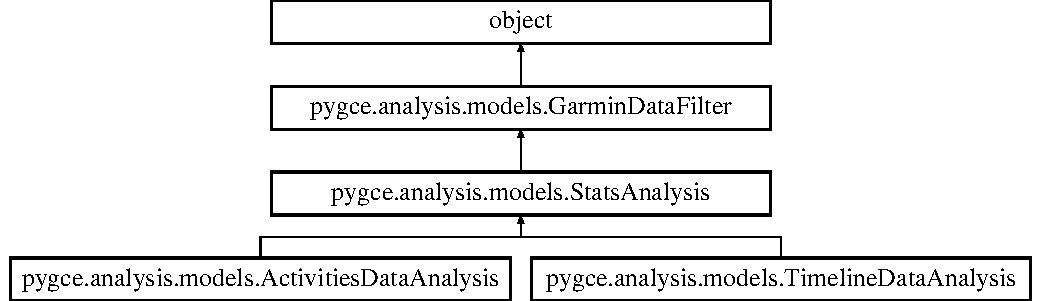
\includegraphics[height=4.000000cm]{classpygce_1_1analysis_1_1models_1_1_garmin_data_filter}
\end{center}
\end{figure}
\subsection*{Public Member Functions}
\begin{DoxyCompactItemize}
\item 
def \hyperlink{classpygce_1_1analysis_1_1models_1_1_garmin_data_filter_ae5dcf7d3dd4f98145960b2a751b163d2}{\+\_\+\+\_\+init\+\_\+\+\_\+} (self, \hyperlink{classpygce_1_1analysis_1_1models_1_1_garmin_data_filter_a7bb7be05577c2d31546e27823a5d11c5}{dataset\+\_\+file})
\item 
def \hyperlink{classpygce_1_1analysis_1_1models_1_1_garmin_data_filter_ae502093f9a92b498b42dd8b0257c22dd}{parse\+\_\+csv} (self)
\end{DoxyCompactItemize}
\subsection*{Static Public Member Functions}
\begin{DoxyCompactItemize}
\item 
def \hyperlink{classpygce_1_1analysis_1_1models_1_1_garmin_data_filter_aba928d8e942c743cf1553760cdb95ea1}{convert\+\_\+time\+\_\+columns} (headers, headers\+\_\+to\+\_\+convert, data)
\item 
def \hyperlink{classpygce_1_1analysis_1_1models_1_1_garmin_data_filter_a7220b9a58e6a9e4fe5dd679b7c8dd3ae}{fix\+\_\+floats} (headers, headers\+\_\+to\+\_\+fix, data)
\end{DoxyCompactItemize}
\subsection*{Public Attributes}
\begin{DoxyCompactItemize}
\item 
\hyperlink{classpygce_1_1analysis_1_1models_1_1_garmin_data_filter_a7bb7be05577c2d31546e27823a5d11c5}{dataset\+\_\+file}
\end{DoxyCompactItemize}


\subsection{Detailed Description}
\begin{DoxyVerb}Parses and fixes raw data \end{DoxyVerb}
 

Definition at line 29 of file models.\+py.



\subsection{Constructor \& Destructor Documentation}
\index{pygce\+::analysis\+::models\+::\+Garmin\+Data\+Filter@{pygce\+::analysis\+::models\+::\+Garmin\+Data\+Filter}!\+\_\+\+\_\+init\+\_\+\+\_\+@{\+\_\+\+\_\+init\+\_\+\+\_\+}}
\index{\+\_\+\+\_\+init\+\_\+\+\_\+@{\+\_\+\+\_\+init\+\_\+\+\_\+}!pygce\+::analysis\+::models\+::\+Garmin\+Data\+Filter@{pygce\+::analysis\+::models\+::\+Garmin\+Data\+Filter}}
\subsubsection[{\texorpdfstring{\+\_\+\+\_\+init\+\_\+\+\_\+(self, dataset\+\_\+file)}{__init__(self, dataset_file)}}]{\setlength{\rightskip}{0pt plus 5cm}def pygce.\+analysis.\+models.\+Garmin\+Data\+Filter.\+\_\+\+\_\+init\+\_\+\+\_\+ (
\begin{DoxyParamCaption}
\item[{}]{self, }
\item[{}]{dataset\+\_\+file}
\end{DoxyParamCaption}
)}\hypertarget{classpygce_1_1analysis_1_1models_1_1_garmin_data_filter_ae5dcf7d3dd4f98145960b2a751b163d2}{}\label{classpygce_1_1analysis_1_1models_1_1_garmin_data_filter_ae5dcf7d3dd4f98145960b2a751b163d2}
\begin{DoxyVerb}:param dataset_file: str
    Path to folder with data to analyse
\end{DoxyVerb}
 

Definition at line 32 of file models.\+py.



\subsection{Member Function Documentation}
\index{pygce\+::analysis\+::models\+::\+Garmin\+Data\+Filter@{pygce\+::analysis\+::models\+::\+Garmin\+Data\+Filter}!convert\+\_\+time\+\_\+columns@{convert\+\_\+time\+\_\+columns}}
\index{convert\+\_\+time\+\_\+columns@{convert\+\_\+time\+\_\+columns}!pygce\+::analysis\+::models\+::\+Garmin\+Data\+Filter@{pygce\+::analysis\+::models\+::\+Garmin\+Data\+Filter}}
\subsubsection[{\texorpdfstring{convert\+\_\+time\+\_\+columns(headers, headers\+\_\+to\+\_\+convert, data)}{convert_time_columns(headers, headers_to_convert, data)}}]{\setlength{\rightskip}{0pt plus 5cm}def pygce.\+analysis.\+models.\+Garmin\+Data\+Filter.\+convert\+\_\+time\+\_\+columns (
\begin{DoxyParamCaption}
\item[{}]{headers, }
\item[{}]{headers\+\_\+to\+\_\+convert, }
\item[{}]{data}
\end{DoxyParamCaption}
)\hspace{0.3cm}{\ttfamily [static]}}\hypertarget{classpygce_1_1analysis_1_1models_1_1_garmin_data_filter_aba928d8e942c743cf1553760cdb95ea1}{}\label{classpygce_1_1analysis_1_1models_1_1_garmin_data_filter_aba928d8e942c743cf1553760cdb95ea1}
\begin{DoxyVerb}:param headers: [] of str
    Column names of data
:param headers_to_convert: [] of str
    Column names of data to convert from time format to float
:param data: [] of []
    Raw data
:return: [] of []
    Input data but with converted time columns
\end{DoxyVerb}
 

Definition at line 51 of file models.\+py.

\index{pygce\+::analysis\+::models\+::\+Garmin\+Data\+Filter@{pygce\+::analysis\+::models\+::\+Garmin\+Data\+Filter}!fix\+\_\+floats@{fix\+\_\+floats}}
\index{fix\+\_\+floats@{fix\+\_\+floats}!pygce\+::analysis\+::models\+::\+Garmin\+Data\+Filter@{pygce\+::analysis\+::models\+::\+Garmin\+Data\+Filter}}
\subsubsection[{\texorpdfstring{fix\+\_\+floats(headers, headers\+\_\+to\+\_\+fix, data)}{fix_floats(headers, headers_to_fix, data)}}]{\setlength{\rightskip}{0pt plus 5cm}def pygce.\+analysis.\+models.\+Garmin\+Data\+Filter.\+fix\+\_\+floats (
\begin{DoxyParamCaption}
\item[{}]{headers, }
\item[{}]{headers\+\_\+to\+\_\+fix, }
\item[{}]{data}
\end{DoxyParamCaption}
)\hspace{0.3cm}{\ttfamily [static]}}\hypertarget{classpygce_1_1analysis_1_1models_1_1_garmin_data_filter_a7220b9a58e6a9e4fe5dd679b7c8dd3ae}{}\label{classpygce_1_1analysis_1_1models_1_1_garmin_data_filter_a7220b9a58e6a9e4fe5dd679b7c8dd3ae}
\begin{DoxyVerb}:param headers: [] of str
    Column names of data
:param headers_to_fix: [] of str
    Column names of data to fix the float format
:param data: [] of []
    Raw data
:return: [] of []
    Input data but with fixed floats in columns
\end{DoxyVerb}
 

Definition at line 71 of file models.\+py.

\index{pygce\+::analysis\+::models\+::\+Garmin\+Data\+Filter@{pygce\+::analysis\+::models\+::\+Garmin\+Data\+Filter}!parse\+\_\+csv@{parse\+\_\+csv}}
\index{parse\+\_\+csv@{parse\+\_\+csv}!pygce\+::analysis\+::models\+::\+Garmin\+Data\+Filter@{pygce\+::analysis\+::models\+::\+Garmin\+Data\+Filter}}
\subsubsection[{\texorpdfstring{parse\+\_\+csv(self)}{parse_csv(self)}}]{\setlength{\rightskip}{0pt plus 5cm}def pygce.\+analysis.\+models.\+Garmin\+Data\+Filter.\+parse\+\_\+csv (
\begin{DoxyParamCaption}
\item[{}]{self}
\end{DoxyParamCaption}
)}\hypertarget{classpygce_1_1analysis_1_1models_1_1_garmin_data_filter_ae502093f9a92b498b42dd8b0257c22dd}{}\label{classpygce_1_1analysis_1_1models_1_1_garmin_data_filter_ae502093f9a92b498b42dd8b0257c22dd}
\begin{DoxyVerb}:return: tuple [], [] of []
    Headers of csv file and data
\end{DoxyVerb}
 

Definition at line 42 of file models.\+py.



\subsection{Member Data Documentation}
\index{pygce\+::analysis\+::models\+::\+Garmin\+Data\+Filter@{pygce\+::analysis\+::models\+::\+Garmin\+Data\+Filter}!dataset\+\_\+file@{dataset\+\_\+file}}
\index{dataset\+\_\+file@{dataset\+\_\+file}!pygce\+::analysis\+::models\+::\+Garmin\+Data\+Filter@{pygce\+::analysis\+::models\+::\+Garmin\+Data\+Filter}}
\subsubsection[{\texorpdfstring{dataset\+\_\+file}{dataset_file}}]{\setlength{\rightskip}{0pt plus 5cm}pygce.\+analysis.\+models.\+Garmin\+Data\+Filter.\+dataset\+\_\+file}\hypertarget{classpygce_1_1analysis_1_1models_1_1_garmin_data_filter_a7bb7be05577c2d31546e27823a5d11c5}{}\label{classpygce_1_1analysis_1_1models_1_1_garmin_data_filter_a7bb7be05577c2d31546e27823a5d11c5}


Definition at line 40 of file models.\+py.



The documentation for this class was generated from the following file\+:\begin{DoxyCompactItemize}
\item 
/home/stefano/\+Coding/\+Python/projects/garmin-\/connect-\/export/pygce/analysis/\hyperlink{models_8py}{models.\+py}\end{DoxyCompactItemize}

\hypertarget{classpygce_1_1models_1_1garmin_1_1timeline_1_1_g_c_day_activities}{}\section{pygce.\+models.\+garmin.\+timeline.\+G\+C\+Day\+Activities Class Reference}
\label{classpygce_1_1models_1_1garmin_1_1timeline_1_1_g_c_day_activities}\index{pygce.\+models.\+garmin.\+timeline.\+G\+C\+Day\+Activities@{pygce.\+models.\+garmin.\+timeline.\+G\+C\+Day\+Activities}}
Inheritance diagram for pygce.\+models.\+garmin.\+timeline.\+G\+C\+Day\+Activities\+:\begin{figure}[H]
\begin{center}
\leavevmode
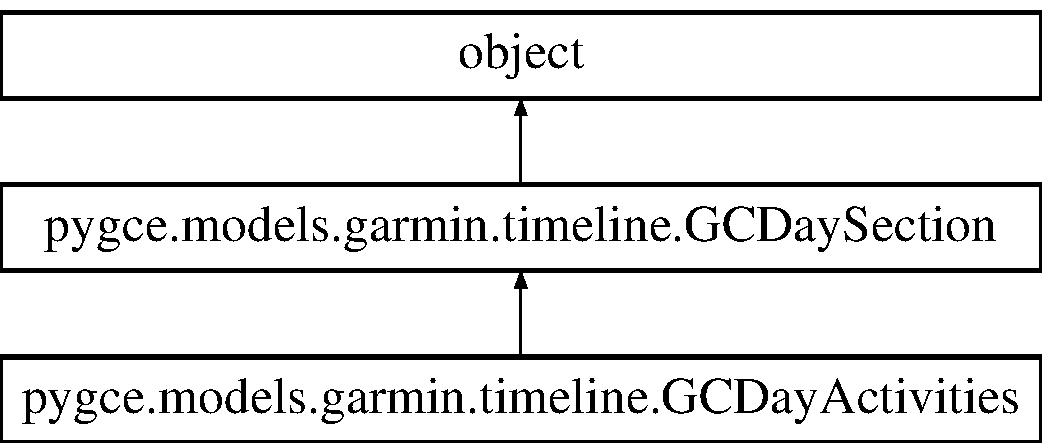
\includegraphics[height=3.000000cm]{classpygce_1_1models_1_1garmin_1_1timeline_1_1_g_c_day_activities}
\end{center}
\end{figure}
\subsection*{Public Member Functions}
\begin{DoxyCompactItemize}
\item 
def \hyperlink{classpygce_1_1models_1_1garmin_1_1timeline_1_1_g_c_day_activities_abde52d1321a233947e2585e7ed43415b}{\+\_\+\+\_\+init\+\_\+\+\_\+} (self, raw\+\_\+html)
\item 
def \hyperlink{classpygce_1_1models_1_1garmin_1_1timeline_1_1_g_c_day_activities_a665d9bc773825c31562129f1f5b47a2c}{parse} (self)
\item 
def \hyperlink{classpygce_1_1models_1_1garmin_1_1timeline_1_1_g_c_day_activities_a6c4869fd929e6076d25e949c7ee51d91}{to\+\_\+dict} (self)
\item 
def \hyperlink{classpygce_1_1models_1_1garmin_1_1timeline_1_1_g_c_day_activities_ab1366ff6ee7b5230f12e6a3f324ffc8f}{to\+\_\+json} (self)
\item 
def \hyperlink{classpygce_1_1models_1_1garmin_1_1timeline_1_1_g_c_day_activities_a2e4d1b6ab08095a558271ba0299c3535}{to\+\_\+csv\+\_\+dict} (self)
\item 
def \hyperlink{classpygce_1_1models_1_1garmin_1_1timeline_1_1_g_c_day_activities_a1f271dd2ea272005fe5dc739496ed9e1}{get\+\_\+total\+\_\+kcal} (self)
\item 
def \hyperlink{classpygce_1_1models_1_1garmin_1_1timeline_1_1_g_c_day_activities_a960ae86a18db046fac6222a3f62e3035}{get\+\_\+total\+\_\+duration} (self)
\item 
def \hyperlink{classpygce_1_1models_1_1garmin_1_1timeline_1_1_g_c_day_activities_a2ad838af777ce178392b5f61ee6e6561}{get\+\_\+total\+\_\+distance} (self)
\item 
def \hyperlink{classpygce_1_1models_1_1garmin_1_1timeline_1_1_g_c_day_activities_a230c1feee2914f86f2bddb05fc2e51cd}{get\+\_\+totals\+\_\+dict} (self)
\end{DoxyCompactItemize}
\subsection*{Static Public Member Functions}
\begin{DoxyCompactItemize}
\item 
def \hyperlink{classpygce_1_1models_1_1garmin_1_1timeline_1_1_g_c_day_activities_a3e5401673c704697c90e814affe368ca}{parse\+\_\+activity} (raw\+\_\+html)
\end{DoxyCompactItemize}
\subsection*{Public Attributes}
\begin{DoxyCompactItemize}
\item 
\hyperlink{classpygce_1_1models_1_1garmin_1_1timeline_1_1_g_c_day_activities_a8f48f44c8208989ea0741bad614ae652}{activities}
\end{DoxyCompactItemize}


\subsection{Detailed Description}
\begin{DoxyVerb}Standard activity in the Garmin Connect timeline of day.
Common features are kcal, time, distance, type, name, link
\end{DoxyVerb}
 

Definition at line 294 of file timeline.\+py.



\subsection{Constructor \& Destructor Documentation}
\index{pygce\+::models\+::garmin\+::timeline\+::\+G\+C\+Day\+Activities@{pygce\+::models\+::garmin\+::timeline\+::\+G\+C\+Day\+Activities}!\+\_\+\+\_\+init\+\_\+\+\_\+@{\+\_\+\+\_\+init\+\_\+\+\_\+}}
\index{\+\_\+\+\_\+init\+\_\+\+\_\+@{\+\_\+\+\_\+init\+\_\+\+\_\+}!pygce\+::models\+::garmin\+::timeline\+::\+G\+C\+Day\+Activities@{pygce\+::models\+::garmin\+::timeline\+::\+G\+C\+Day\+Activities}}
\subsubsection[{\texorpdfstring{\+\_\+\+\_\+init\+\_\+\+\_\+(self, raw\+\_\+html)}{__init__(self, raw_html)}}]{\setlength{\rightskip}{0pt plus 5cm}def pygce.\+models.\+garmin.\+timeline.\+G\+C\+Day\+Activities.\+\_\+\+\_\+init\+\_\+\+\_\+ (
\begin{DoxyParamCaption}
\item[{}]{self, }
\item[{}]{raw\+\_\+html}
\end{DoxyParamCaption}
)}\hypertarget{classpygce_1_1models_1_1garmin_1_1timeline_1_1_g_c_day_activities_abde52d1321a233947e2585e7ed43415b}{}\label{classpygce_1_1models_1_1garmin_1_1timeline_1_1_g_c_day_activities_abde52d1321a233947e2585e7ed43415b}
\begin{DoxyVerb}:param raw_html: str
    HTML source snippet with information about section
\end{DoxyVerb}
 

Definition at line 300 of file timeline.\+py.



\subsection{Member Function Documentation}
\index{pygce\+::models\+::garmin\+::timeline\+::\+G\+C\+Day\+Activities@{pygce\+::models\+::garmin\+::timeline\+::\+G\+C\+Day\+Activities}!get\+\_\+total\+\_\+distance@{get\+\_\+total\+\_\+distance}}
\index{get\+\_\+total\+\_\+distance@{get\+\_\+total\+\_\+distance}!pygce\+::models\+::garmin\+::timeline\+::\+G\+C\+Day\+Activities@{pygce\+::models\+::garmin\+::timeline\+::\+G\+C\+Day\+Activities}}
\subsubsection[{\texorpdfstring{get\+\_\+total\+\_\+distance(self)}{get_total_distance(self)}}]{\setlength{\rightskip}{0pt plus 5cm}def pygce.\+models.\+garmin.\+timeline.\+G\+C\+Day\+Activities.\+get\+\_\+total\+\_\+distance (
\begin{DoxyParamCaption}
\item[{}]{self}
\end{DoxyParamCaption}
)}\hypertarget{classpygce_1_1models_1_1garmin_1_1timeline_1_1_g_c_day_activities_a2ad838af777ce178392b5f61ee6e6561}{}\label{classpygce_1_1models_1_1garmin_1_1timeline_1_1_g_c_day_activities_a2ad838af777ce178392b5f61ee6e6561}
\begin{DoxyVerb}:return: float
    Total distance of all activities
\end{DoxyVerb}
 

Definition at line 400 of file timeline.\+py.

\index{pygce\+::models\+::garmin\+::timeline\+::\+G\+C\+Day\+Activities@{pygce\+::models\+::garmin\+::timeline\+::\+G\+C\+Day\+Activities}!get\+\_\+total\+\_\+duration@{get\+\_\+total\+\_\+duration}}
\index{get\+\_\+total\+\_\+duration@{get\+\_\+total\+\_\+duration}!pygce\+::models\+::garmin\+::timeline\+::\+G\+C\+Day\+Activities@{pygce\+::models\+::garmin\+::timeline\+::\+G\+C\+Day\+Activities}}
\subsubsection[{\texorpdfstring{get\+\_\+total\+\_\+duration(self)}{get_total_duration(self)}}]{\setlength{\rightskip}{0pt plus 5cm}def pygce.\+models.\+garmin.\+timeline.\+G\+C\+Day\+Activities.\+get\+\_\+total\+\_\+duration (
\begin{DoxyParamCaption}
\item[{}]{self}
\end{DoxyParamCaption}
)}\hypertarget{classpygce_1_1models_1_1garmin_1_1timeline_1_1_g_c_day_activities_a960ae86a18db046fac6222a3f62e3035}{}\label{classpygce_1_1models_1_1garmin_1_1timeline_1_1_g_c_day_activities_a960ae86a18db046fac6222a3f62e3035}
\begin{DoxyVerb}:return: timedelta
    Total duration of all activities
\end{DoxyVerb}
 

Definition at line 387 of file timeline.\+py.

\index{pygce\+::models\+::garmin\+::timeline\+::\+G\+C\+Day\+Activities@{pygce\+::models\+::garmin\+::timeline\+::\+G\+C\+Day\+Activities}!get\+\_\+total\+\_\+kcal@{get\+\_\+total\+\_\+kcal}}
\index{get\+\_\+total\+\_\+kcal@{get\+\_\+total\+\_\+kcal}!pygce\+::models\+::garmin\+::timeline\+::\+G\+C\+Day\+Activities@{pygce\+::models\+::garmin\+::timeline\+::\+G\+C\+Day\+Activities}}
\subsubsection[{\texorpdfstring{get\+\_\+total\+\_\+kcal(self)}{get_total_kcal(self)}}]{\setlength{\rightskip}{0pt plus 5cm}def pygce.\+models.\+garmin.\+timeline.\+G\+C\+Day\+Activities.\+get\+\_\+total\+\_\+kcal (
\begin{DoxyParamCaption}
\item[{}]{self}
\end{DoxyParamCaption}
)}\hypertarget{classpygce_1_1models_1_1garmin_1_1timeline_1_1_g_c_day_activities_a1f271dd2ea272005fe5dc739496ed9e1}{}\label{classpygce_1_1models_1_1garmin_1_1timeline_1_1_g_c_day_activities_a1f271dd2ea272005fe5dc739496ed9e1}
\begin{DoxyVerb}:return: float
    Total kcal of all activities
\end{DoxyVerb}
 

Definition at line 379 of file timeline.\+py.

\index{pygce\+::models\+::garmin\+::timeline\+::\+G\+C\+Day\+Activities@{pygce\+::models\+::garmin\+::timeline\+::\+G\+C\+Day\+Activities}!get\+\_\+totals\+\_\+dict@{get\+\_\+totals\+\_\+dict}}
\index{get\+\_\+totals\+\_\+dict@{get\+\_\+totals\+\_\+dict}!pygce\+::models\+::garmin\+::timeline\+::\+G\+C\+Day\+Activities@{pygce\+::models\+::garmin\+::timeline\+::\+G\+C\+Day\+Activities}}
\subsubsection[{\texorpdfstring{get\+\_\+totals\+\_\+dict(self)}{get_totals_dict(self)}}]{\setlength{\rightskip}{0pt plus 5cm}def pygce.\+models.\+garmin.\+timeline.\+G\+C\+Day\+Activities.\+get\+\_\+totals\+\_\+dict (
\begin{DoxyParamCaption}
\item[{}]{self}
\end{DoxyParamCaption}
)}\hypertarget{classpygce_1_1models_1_1garmin_1_1timeline_1_1_g_c_day_activities_a230c1feee2914f86f2bddb05fc2e51cd}{}\label{classpygce_1_1models_1_1garmin_1_1timeline_1_1_g_c_day_activities_a230c1feee2914f86f2bddb05fc2e51cd}
\begin{DoxyVerb}:return: {}
    Self dict but with totals instead (total kcal, total distance ...)
\end{DoxyVerb}
 

Definition at line 408 of file timeline.\+py.

\index{pygce\+::models\+::garmin\+::timeline\+::\+G\+C\+Day\+Activities@{pygce\+::models\+::garmin\+::timeline\+::\+G\+C\+Day\+Activities}!parse@{parse}}
\index{parse@{parse}!pygce\+::models\+::garmin\+::timeline\+::\+G\+C\+Day\+Activities@{pygce\+::models\+::garmin\+::timeline\+::\+G\+C\+Day\+Activities}}
\subsubsection[{\texorpdfstring{parse(self)}{parse(self)}}]{\setlength{\rightskip}{0pt plus 5cm}def pygce.\+models.\+garmin.\+timeline.\+G\+C\+Day\+Activities.\+parse (
\begin{DoxyParamCaption}
\item[{}]{self}
\end{DoxyParamCaption}
)}\hypertarget{classpygce_1_1models_1_1garmin_1_1timeline_1_1_g_c_day_activities_a665d9bc773825c31562129f1f5b47a2c}{}\label{classpygce_1_1models_1_1garmin_1_1timeline_1_1_g_c_day_activities_a665d9bc773825c31562129f1f5b47a2c}


Definition at line 310 of file timeline.\+py.

\index{pygce\+::models\+::garmin\+::timeline\+::\+G\+C\+Day\+Activities@{pygce\+::models\+::garmin\+::timeline\+::\+G\+C\+Day\+Activities}!parse\+\_\+activity@{parse\+\_\+activity}}
\index{parse\+\_\+activity@{parse\+\_\+activity}!pygce\+::models\+::garmin\+::timeline\+::\+G\+C\+Day\+Activities@{pygce\+::models\+::garmin\+::timeline\+::\+G\+C\+Day\+Activities}}
\subsubsection[{\texorpdfstring{parse\+\_\+activity(raw\+\_\+html)}{parse_activity(raw_html)}}]{\setlength{\rightskip}{0pt plus 5cm}def pygce.\+models.\+garmin.\+timeline.\+G\+C\+Day\+Activities.\+parse\+\_\+activity (
\begin{DoxyParamCaption}
\item[{}]{raw\+\_\+html}
\end{DoxyParamCaption}
)\hspace{0.3cm}{\ttfamily [static]}}\hypertarget{classpygce_1_1models_1_1garmin_1_1timeline_1_1_g_c_day_activities_a3e5401673c704697c90e814affe368ca}{}\label{classpygce_1_1models_1_1garmin_1_1timeline_1_1_g_c_day_activities_a3e5401673c704697c90e814affe368ca}
\begin{DoxyVerb}:param raw_html: str html code
    Raw HTML code of row of table containing activity to parse
:return: dict
    Dict with values of activity
\end{DoxyVerb}
 

Definition at line 317 of file timeline.\+py.

\index{pygce\+::models\+::garmin\+::timeline\+::\+G\+C\+Day\+Activities@{pygce\+::models\+::garmin\+::timeline\+::\+G\+C\+Day\+Activities}!to\+\_\+csv\+\_\+dict@{to\+\_\+csv\+\_\+dict}}
\index{to\+\_\+csv\+\_\+dict@{to\+\_\+csv\+\_\+dict}!pygce\+::models\+::garmin\+::timeline\+::\+G\+C\+Day\+Activities@{pygce\+::models\+::garmin\+::timeline\+::\+G\+C\+Day\+Activities}}
\subsubsection[{\texorpdfstring{to\+\_\+csv\+\_\+dict(self)}{to_csv_dict(self)}}]{\setlength{\rightskip}{0pt plus 5cm}def pygce.\+models.\+garmin.\+timeline.\+G\+C\+Day\+Activities.\+to\+\_\+csv\+\_\+dict (
\begin{DoxyParamCaption}
\item[{}]{self}
\end{DoxyParamCaption}
)}\hypertarget{classpygce_1_1models_1_1garmin_1_1timeline_1_1_g_c_day_activities_a2e4d1b6ab08095a558271ba0299c3535}{}\label{classpygce_1_1models_1_1garmin_1_1timeline_1_1_g_c_day_activities_a2e4d1b6ab08095a558271ba0299c3535}
\begin{DoxyVerb}:return: {}
    Like super.to_csv_dict() but with totals instead
\end{DoxyVerb}
 

Definition at line 366 of file timeline.\+py.

\index{pygce\+::models\+::garmin\+::timeline\+::\+G\+C\+Day\+Activities@{pygce\+::models\+::garmin\+::timeline\+::\+G\+C\+Day\+Activities}!to\+\_\+dict@{to\+\_\+dict}}
\index{to\+\_\+dict@{to\+\_\+dict}!pygce\+::models\+::garmin\+::timeline\+::\+G\+C\+Day\+Activities@{pygce\+::models\+::garmin\+::timeline\+::\+G\+C\+Day\+Activities}}
\subsubsection[{\texorpdfstring{to\+\_\+dict(self)}{to_dict(self)}}]{\setlength{\rightskip}{0pt plus 5cm}def pygce.\+models.\+garmin.\+timeline.\+G\+C\+Day\+Activities.\+to\+\_\+dict (
\begin{DoxyParamCaption}
\item[{}]{self}
\end{DoxyParamCaption}
)}\hypertarget{classpygce_1_1models_1_1garmin_1_1timeline_1_1_g_c_day_activities_a6c4869fd929e6076d25e949c7ee51d91}{}\label{classpygce_1_1models_1_1garmin_1_1timeline_1_1_g_c_day_activities_a6c4869fd929e6076d25e949c7ee51d91}


Definition at line 353 of file timeline.\+py.

\index{pygce\+::models\+::garmin\+::timeline\+::\+G\+C\+Day\+Activities@{pygce\+::models\+::garmin\+::timeline\+::\+G\+C\+Day\+Activities}!to\+\_\+json@{to\+\_\+json}}
\index{to\+\_\+json@{to\+\_\+json}!pygce\+::models\+::garmin\+::timeline\+::\+G\+C\+Day\+Activities@{pygce\+::models\+::garmin\+::timeline\+::\+G\+C\+Day\+Activities}}
\subsubsection[{\texorpdfstring{to\+\_\+json(self)}{to_json(self)}}]{\setlength{\rightskip}{0pt plus 5cm}def pygce.\+models.\+garmin.\+timeline.\+G\+C\+Day\+Activities.\+to\+\_\+json (
\begin{DoxyParamCaption}
\item[{}]{self}
\end{DoxyParamCaption}
)}\hypertarget{classpygce_1_1models_1_1garmin_1_1timeline_1_1_g_c_day_activities_ab1366ff6ee7b5230f12e6a3f324ffc8f}{}\label{classpygce_1_1models_1_1garmin_1_1timeline_1_1_g_c_day_activities_ab1366ff6ee7b5230f12e6a3f324ffc8f}


Definition at line 358 of file timeline.\+py.



\subsection{Member Data Documentation}
\index{pygce\+::models\+::garmin\+::timeline\+::\+G\+C\+Day\+Activities@{pygce\+::models\+::garmin\+::timeline\+::\+G\+C\+Day\+Activities}!activities@{activities}}
\index{activities@{activities}!pygce\+::models\+::garmin\+::timeline\+::\+G\+C\+Day\+Activities@{pygce\+::models\+::garmin\+::timeline\+::\+G\+C\+Day\+Activities}}
\subsubsection[{\texorpdfstring{activities}{activities}}]{\setlength{\rightskip}{0pt plus 5cm}pygce.\+models.\+garmin.\+timeline.\+G\+C\+Day\+Activities.\+activities}\hypertarget{classpygce_1_1models_1_1garmin_1_1timeline_1_1_g_c_day_activities_a8f48f44c8208989ea0741bad614ae652}{}\label{classpygce_1_1models_1_1garmin_1_1timeline_1_1_g_c_day_activities_a8f48f44c8208989ea0741bad614ae652}


Definition at line 308 of file timeline.\+py.



The documentation for this class was generated from the following file\+:\begin{DoxyCompactItemize}
\item 
/home/stefano/\+Coding/\+Python/projects/garmin-\/connect-\/export/pygce/models/garmin/\hyperlink{timeline_8py}{timeline.\+py}\end{DoxyCompactItemize}

\hypertarget{classpygce_1_1models_1_1garmin_1_1timeline_1_1_g_c_day_breakdown}{}\section{pygce.\+models.\+garmin.\+timeline.\+G\+C\+Day\+Breakdown Class Reference}
\label{classpygce_1_1models_1_1garmin_1_1timeline_1_1_g_c_day_breakdown}\index{pygce.\+models.\+garmin.\+timeline.\+G\+C\+Day\+Breakdown@{pygce.\+models.\+garmin.\+timeline.\+G\+C\+Day\+Breakdown}}
Inheritance diagram for pygce.\+models.\+garmin.\+timeline.\+G\+C\+Day\+Breakdown\+:\begin{figure}[H]
\begin{center}
\leavevmode
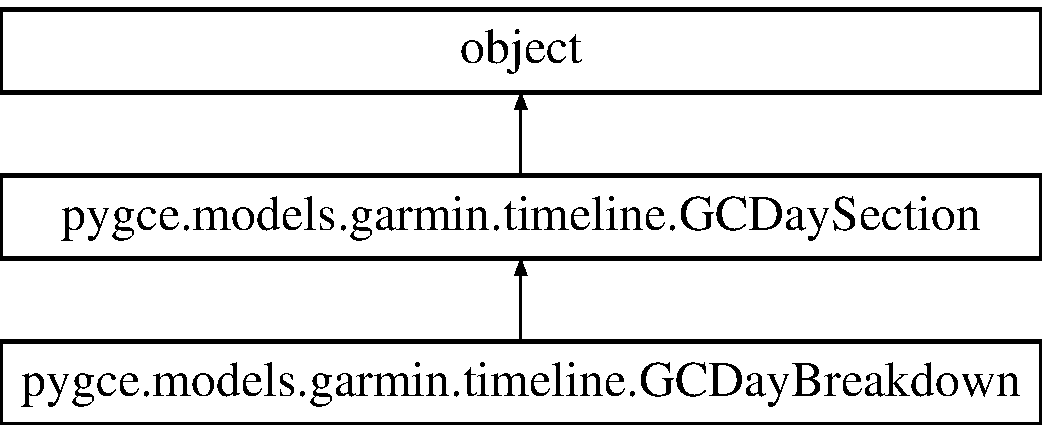
\includegraphics[height=3.000000cm]{classpygce_1_1models_1_1garmin_1_1timeline_1_1_g_c_day_breakdown}
\end{center}
\end{figure}
\subsection*{Public Member Functions}
\begin{DoxyCompactItemize}
\item 
def \hyperlink{classpygce_1_1models_1_1garmin_1_1timeline_1_1_g_c_day_breakdown_af19f3c3dad89dff7f543be029b0778f7}{\+\_\+\+\_\+init\+\_\+\+\_\+} (self, raw\+\_\+html)
\item 
def \hyperlink{classpygce_1_1models_1_1garmin_1_1timeline_1_1_g_c_day_breakdown_aac05cc21c76e377ad50dcfcaca3a54da}{parse} (self)
\item 
def \hyperlink{classpygce_1_1models_1_1garmin_1_1timeline_1_1_g_c_day_breakdown_a517a2e5b269e95331fb51f531a5b9e4b}{to\+\_\+dict} (self)
\end{DoxyCompactItemize}
\subsection*{Public Attributes}
\begin{DoxyCompactItemize}
\item 
\hyperlink{classpygce_1_1models_1_1garmin_1_1timeline_1_1_g_c_day_breakdown_a736edad716e1770862ceac10f2d262e3}{highly\+\_\+active}
\item 
\hyperlink{classpygce_1_1models_1_1garmin_1_1timeline_1_1_g_c_day_breakdown_afabd12a8a6d22c156f9495483e4419b6}{active}
\item 
\hyperlink{classpygce_1_1models_1_1garmin_1_1timeline_1_1_g_c_day_breakdown_a03d898e7c3c8131ff30e0316d7257739}{sedentary}
\item 
\hyperlink{classpygce_1_1models_1_1garmin_1_1timeline_1_1_g_c_day_breakdown_a26a3f7d4d5903c8ad6221c11ded6d601}{sleeping}
\end{DoxyCompactItemize}


\subsection{Detailed Description}
\begin{DoxyVerb}Standard activity in the Garmin Connect timeline of day.
Common features are highly active %, active %, sedentary %, sleep %
\end{DoxyVerb}
 

Definition at line 451 of file timeline.\+py.



\subsection{Constructor \& Destructor Documentation}
\mbox{\Hypertarget{classpygce_1_1models_1_1garmin_1_1timeline_1_1_g_c_day_breakdown_af19f3c3dad89dff7f543be029b0778f7}\label{classpygce_1_1models_1_1garmin_1_1timeline_1_1_g_c_day_breakdown_af19f3c3dad89dff7f543be029b0778f7}} 
\index{pygce\+::models\+::garmin\+::timeline\+::\+G\+C\+Day\+Breakdown@{pygce\+::models\+::garmin\+::timeline\+::\+G\+C\+Day\+Breakdown}!\+\_\+\+\_\+init\+\_\+\+\_\+@{\+\_\+\+\_\+init\+\_\+\+\_\+}}
\index{\+\_\+\+\_\+init\+\_\+\+\_\+@{\+\_\+\+\_\+init\+\_\+\+\_\+}!pygce\+::models\+::garmin\+::timeline\+::\+G\+C\+Day\+Breakdown@{pygce\+::models\+::garmin\+::timeline\+::\+G\+C\+Day\+Breakdown}}
\subsubsection{\texorpdfstring{\+\_\+\+\_\+init\+\_\+\+\_\+()}{\_\_init\_\_()}}
{\footnotesize\ttfamily def pygce.\+models.\+garmin.\+timeline.\+G\+C\+Day\+Breakdown.\+\_\+\+\_\+init\+\_\+\+\_\+ (\begin{DoxyParamCaption}\item[{}]{self,  }\item[{}]{raw\+\_\+html }\end{DoxyParamCaption})}

\begin{DoxyVerb}:param raw_html: str
    HTML source snippet with information about section
\end{DoxyVerb}
 

Definition at line 457 of file timeline.\+py.



\subsection{Member Function Documentation}
\mbox{\Hypertarget{classpygce_1_1models_1_1garmin_1_1timeline_1_1_g_c_day_breakdown_aac05cc21c76e377ad50dcfcaca3a54da}\label{classpygce_1_1models_1_1garmin_1_1timeline_1_1_g_c_day_breakdown_aac05cc21c76e377ad50dcfcaca3a54da}} 
\index{pygce\+::models\+::garmin\+::timeline\+::\+G\+C\+Day\+Breakdown@{pygce\+::models\+::garmin\+::timeline\+::\+G\+C\+Day\+Breakdown}!parse@{parse}}
\index{parse@{parse}!pygce\+::models\+::garmin\+::timeline\+::\+G\+C\+Day\+Breakdown@{pygce\+::models\+::garmin\+::timeline\+::\+G\+C\+Day\+Breakdown}}
\subsubsection{\texorpdfstring{parse()}{parse()}}
{\footnotesize\ttfamily def pygce.\+models.\+garmin.\+timeline.\+G\+C\+Day\+Breakdown.\+parse (\begin{DoxyParamCaption}\item[{}]{self }\end{DoxyParamCaption})}



Definition at line 470 of file timeline.\+py.

\mbox{\Hypertarget{classpygce_1_1models_1_1garmin_1_1timeline_1_1_g_c_day_breakdown_a517a2e5b269e95331fb51f531a5b9e4b}\label{classpygce_1_1models_1_1garmin_1_1timeline_1_1_g_c_day_breakdown_a517a2e5b269e95331fb51f531a5b9e4b}} 
\index{pygce\+::models\+::garmin\+::timeline\+::\+G\+C\+Day\+Breakdown@{pygce\+::models\+::garmin\+::timeline\+::\+G\+C\+Day\+Breakdown}!to\+\_\+dict@{to\+\_\+dict}}
\index{to\+\_\+dict@{to\+\_\+dict}!pygce\+::models\+::garmin\+::timeline\+::\+G\+C\+Day\+Breakdown@{pygce\+::models\+::garmin\+::timeline\+::\+G\+C\+Day\+Breakdown}}
\subsubsection{\texorpdfstring{to\+\_\+dict()}{to\_dict()}}
{\footnotesize\ttfamily def pygce.\+models.\+garmin.\+timeline.\+G\+C\+Day\+Breakdown.\+to\+\_\+dict (\begin{DoxyParamCaption}\item[{}]{self }\end{DoxyParamCaption})}



Definition at line 495 of file timeline.\+py.



\subsection{Member Data Documentation}
\mbox{\Hypertarget{classpygce_1_1models_1_1garmin_1_1timeline_1_1_g_c_day_breakdown_afabd12a8a6d22c156f9495483e4419b6}\label{classpygce_1_1models_1_1garmin_1_1timeline_1_1_g_c_day_breakdown_afabd12a8a6d22c156f9495483e4419b6}} 
\index{pygce\+::models\+::garmin\+::timeline\+::\+G\+C\+Day\+Breakdown@{pygce\+::models\+::garmin\+::timeline\+::\+G\+C\+Day\+Breakdown}!active@{active}}
\index{active@{active}!pygce\+::models\+::garmin\+::timeline\+::\+G\+C\+Day\+Breakdown@{pygce\+::models\+::garmin\+::timeline\+::\+G\+C\+Day\+Breakdown}}
\subsubsection{\texorpdfstring{active}{active}}
{\footnotesize\ttfamily pygce.\+models.\+garmin.\+timeline.\+G\+C\+Day\+Breakdown.\+active}



Definition at line 466 of file timeline.\+py.

\mbox{\Hypertarget{classpygce_1_1models_1_1garmin_1_1timeline_1_1_g_c_day_breakdown_a736edad716e1770862ceac10f2d262e3}\label{classpygce_1_1models_1_1garmin_1_1timeline_1_1_g_c_day_breakdown_a736edad716e1770862ceac10f2d262e3}} 
\index{pygce\+::models\+::garmin\+::timeline\+::\+G\+C\+Day\+Breakdown@{pygce\+::models\+::garmin\+::timeline\+::\+G\+C\+Day\+Breakdown}!highly\+\_\+active@{highly\+\_\+active}}
\index{highly\+\_\+active@{highly\+\_\+active}!pygce\+::models\+::garmin\+::timeline\+::\+G\+C\+Day\+Breakdown@{pygce\+::models\+::garmin\+::timeline\+::\+G\+C\+Day\+Breakdown}}
\subsubsection{\texorpdfstring{highly\+\_\+active}{highly\_active}}
{\footnotesize\ttfamily pygce.\+models.\+garmin.\+timeline.\+G\+C\+Day\+Breakdown.\+highly\+\_\+active}



Definition at line 465 of file timeline.\+py.

\mbox{\Hypertarget{classpygce_1_1models_1_1garmin_1_1timeline_1_1_g_c_day_breakdown_a03d898e7c3c8131ff30e0316d7257739}\label{classpygce_1_1models_1_1garmin_1_1timeline_1_1_g_c_day_breakdown_a03d898e7c3c8131ff30e0316d7257739}} 
\index{pygce\+::models\+::garmin\+::timeline\+::\+G\+C\+Day\+Breakdown@{pygce\+::models\+::garmin\+::timeline\+::\+G\+C\+Day\+Breakdown}!sedentary@{sedentary}}
\index{sedentary@{sedentary}!pygce\+::models\+::garmin\+::timeline\+::\+G\+C\+Day\+Breakdown@{pygce\+::models\+::garmin\+::timeline\+::\+G\+C\+Day\+Breakdown}}
\subsubsection{\texorpdfstring{sedentary}{sedentary}}
{\footnotesize\ttfamily pygce.\+models.\+garmin.\+timeline.\+G\+C\+Day\+Breakdown.\+sedentary}



Definition at line 467 of file timeline.\+py.

\mbox{\Hypertarget{classpygce_1_1models_1_1garmin_1_1timeline_1_1_g_c_day_breakdown_a26a3f7d4d5903c8ad6221c11ded6d601}\label{classpygce_1_1models_1_1garmin_1_1timeline_1_1_g_c_day_breakdown_a26a3f7d4d5903c8ad6221c11ded6d601}} 
\index{pygce\+::models\+::garmin\+::timeline\+::\+G\+C\+Day\+Breakdown@{pygce\+::models\+::garmin\+::timeline\+::\+G\+C\+Day\+Breakdown}!sleeping@{sleeping}}
\index{sleeping@{sleeping}!pygce\+::models\+::garmin\+::timeline\+::\+G\+C\+Day\+Breakdown@{pygce\+::models\+::garmin\+::timeline\+::\+G\+C\+Day\+Breakdown}}
\subsubsection{\texorpdfstring{sleeping}{sleeping}}
{\footnotesize\ttfamily pygce.\+models.\+garmin.\+timeline.\+G\+C\+Day\+Breakdown.\+sleeping}



Definition at line 468 of file timeline.\+py.



The documentation for this class was generated from the following file\+:\begin{DoxyCompactItemize}
\item 
/home/stefano/\+Coding/\+Python/projects/pygce/pygce/models/garmin/\hyperlink{timeline_8py}{timeline.\+py}\end{DoxyCompactItemize}

\hypertarget{classpygce_1_1models_1_1garmin_1_1timeline_1_1_g_c_day_section}{}\section{pygce.\+models.\+garmin.\+timeline.\+G\+C\+Day\+Section Class Reference}
\label{classpygce_1_1models_1_1garmin_1_1timeline_1_1_g_c_day_section}\index{pygce.\+models.\+garmin.\+timeline.\+G\+C\+Day\+Section@{pygce.\+models.\+garmin.\+timeline.\+G\+C\+Day\+Section}}
Inheritance diagram for pygce.\+models.\+garmin.\+timeline.\+G\+C\+Day\+Section\+:\begin{figure}[H]
\begin{center}
\leavevmode
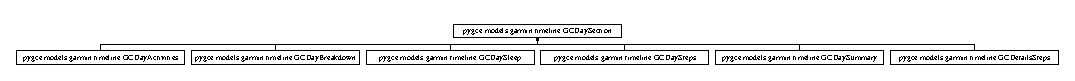
\includegraphics[height=1.142857cm]{classpygce_1_1models_1_1garmin_1_1timeline_1_1_g_c_day_section}
\end{center}
\end{figure}
\subsection*{Public Member Functions}
\begin{DoxyCompactItemize}
\item 
def \hyperlink{classpygce_1_1models_1_1garmin_1_1timeline_1_1_g_c_day_section_aae8c8c4a74381fa4ee47881ad498fb8f}{\+\_\+\+\_\+init\+\_\+\+\_\+} (self, raw\+\_\+html, \hyperlink{classpygce_1_1models_1_1garmin_1_1timeline_1_1_g_c_day_section_a3dacbeacfedec2f69dcbb9fe6870f8a3}{tag}=\char`\"{}\char`\"{})
\item 
def \hyperlink{classpygce_1_1models_1_1garmin_1_1timeline_1_1_g_c_day_section_ac1ddb2f5379e356e93166d1ea934b9c9}{parse} (self)
\item 
def \hyperlink{classpygce_1_1models_1_1garmin_1_1timeline_1_1_g_c_day_section_adf3f25be05c84b2fc99d22cb5014e68d}{to\+\_\+dict} (self)
\item 
def \hyperlink{classpygce_1_1models_1_1garmin_1_1timeline_1_1_g_c_day_section_a810c65491986e687542ee5a4f02c51d7}{to\+\_\+json} (self)
\item 
def \hyperlink{classpygce_1_1models_1_1garmin_1_1timeline_1_1_g_c_day_section_a3a8d885a0155c9fa13843609fb7bf80d}{to\+\_\+csv\+\_\+dict} (self)
\end{DoxyCompactItemize}
\subsection*{Public Attributes}
\begin{DoxyCompactItemize}
\item 
\hyperlink{classpygce_1_1models_1_1garmin_1_1timeline_1_1_g_c_day_section_a3dacbeacfedec2f69dcbb9fe6870f8a3}{tag}
\item 
\hyperlink{classpygce_1_1models_1_1garmin_1_1timeline_1_1_g_c_day_section_ac70b12b38ec07c1afbd3198a2620fe86}{html}
\item 
\hyperlink{classpygce_1_1models_1_1garmin_1_1timeline_1_1_g_c_day_section_ae04dcff466d78ae686dce462057260a9}{soup}
\end{DoxyCompactItemize}


\subsection{Detailed Description}
\begin{DoxyVerb}Standard section in the Garmin Connect timeline of day.
\end{DoxyVerb}
 

Definition at line 13 of file timeline.\+py.



\subsection{Constructor \& Destructor Documentation}
\mbox{\Hypertarget{classpygce_1_1models_1_1garmin_1_1timeline_1_1_g_c_day_section_aae8c8c4a74381fa4ee47881ad498fb8f}\label{classpygce_1_1models_1_1garmin_1_1timeline_1_1_g_c_day_section_aae8c8c4a74381fa4ee47881ad498fb8f}} 
\index{pygce\+::models\+::garmin\+::timeline\+::\+G\+C\+Day\+Section@{pygce\+::models\+::garmin\+::timeline\+::\+G\+C\+Day\+Section}!\+\_\+\+\_\+init\+\_\+\+\_\+@{\+\_\+\+\_\+init\+\_\+\+\_\+}}
\index{\+\_\+\+\_\+init\+\_\+\+\_\+@{\+\_\+\+\_\+init\+\_\+\+\_\+}!pygce\+::models\+::garmin\+::timeline\+::\+G\+C\+Day\+Section@{pygce\+::models\+::garmin\+::timeline\+::\+G\+C\+Day\+Section}}
\subsubsection{\texorpdfstring{\+\_\+\+\_\+init\+\_\+\+\_\+()}{\_\_init\_\_()}}
{\footnotesize\ttfamily def pygce.\+models.\+garmin.\+timeline.\+G\+C\+Day\+Section.\+\_\+\+\_\+init\+\_\+\+\_\+ (\begin{DoxyParamCaption}\item[{}]{self,  }\item[{}]{raw\+\_\+html,  }\item[{}]{tag = {\ttfamily \char`\"{}\char`\"{}} }\end{DoxyParamCaption})}

\begin{DoxyVerb}:param raw_html: str
    HTML source snippet with information about section
:param tag: str
    Unique str in order not to mistake this GCDaySection with another one
\end{DoxyVerb}
 

Definition at line 18 of file timeline.\+py.



\subsection{Member Function Documentation}
\mbox{\Hypertarget{classpygce_1_1models_1_1garmin_1_1timeline_1_1_g_c_day_section_ac1ddb2f5379e356e93166d1ea934b9c9}\label{classpygce_1_1models_1_1garmin_1_1timeline_1_1_g_c_day_section_ac1ddb2f5379e356e93166d1ea934b9c9}} 
\index{pygce\+::models\+::garmin\+::timeline\+::\+G\+C\+Day\+Section@{pygce\+::models\+::garmin\+::timeline\+::\+G\+C\+Day\+Section}!parse@{parse}}
\index{parse@{parse}!pygce\+::models\+::garmin\+::timeline\+::\+G\+C\+Day\+Section@{pygce\+::models\+::garmin\+::timeline\+::\+G\+C\+Day\+Section}}
\subsubsection{\texorpdfstring{parse()}{parse()}}
{\footnotesize\ttfamily def pygce.\+models.\+garmin.\+timeline.\+G\+C\+Day\+Section.\+parse (\begin{DoxyParamCaption}\item[{}]{self }\end{DoxyParamCaption})}

\begin{DoxyVerb}:return: void
    Parses raw html source and tries to finds all information
\end{DoxyVerb}
 

Definition at line 32 of file timeline.\+py.

\mbox{\Hypertarget{classpygce_1_1models_1_1garmin_1_1timeline_1_1_g_c_day_section_a3a8d885a0155c9fa13843609fb7bf80d}\label{classpygce_1_1models_1_1garmin_1_1timeline_1_1_g_c_day_section_a3a8d885a0155c9fa13843609fb7bf80d}} 
\index{pygce\+::models\+::garmin\+::timeline\+::\+G\+C\+Day\+Section@{pygce\+::models\+::garmin\+::timeline\+::\+G\+C\+Day\+Section}!to\+\_\+csv\+\_\+dict@{to\+\_\+csv\+\_\+dict}}
\index{to\+\_\+csv\+\_\+dict@{to\+\_\+csv\+\_\+dict}!pygce\+::models\+::garmin\+::timeline\+::\+G\+C\+Day\+Section@{pygce\+::models\+::garmin\+::timeline\+::\+G\+C\+Day\+Section}}
\subsubsection{\texorpdfstring{to\+\_\+csv\+\_\+dict()}{to\_csv\_dict()}}
{\footnotesize\ttfamily def pygce.\+models.\+garmin.\+timeline.\+G\+C\+Day\+Section.\+to\+\_\+csv\+\_\+dict (\begin{DoxyParamCaption}\item[{}]{self }\end{DoxyParamCaption})}

\begin{DoxyVerb}:return: {}
    Like self.to_json() but with a unique str before each key to spot against different GCDaySections
\end{DoxyVerb}
 

Definition at line 58 of file timeline.\+py.

\mbox{\Hypertarget{classpygce_1_1models_1_1garmin_1_1timeline_1_1_g_c_day_section_adf3f25be05c84b2fc99d22cb5014e68d}\label{classpygce_1_1models_1_1garmin_1_1timeline_1_1_g_c_day_section_adf3f25be05c84b2fc99d22cb5014e68d}} 
\index{pygce\+::models\+::garmin\+::timeline\+::\+G\+C\+Day\+Section@{pygce\+::models\+::garmin\+::timeline\+::\+G\+C\+Day\+Section}!to\+\_\+dict@{to\+\_\+dict}}
\index{to\+\_\+dict@{to\+\_\+dict}!pygce\+::models\+::garmin\+::timeline\+::\+G\+C\+Day\+Section@{pygce\+::models\+::garmin\+::timeline\+::\+G\+C\+Day\+Section}}
\subsubsection{\texorpdfstring{to\+\_\+dict()}{to\_dict()}}
{\footnotesize\ttfamily def pygce.\+models.\+garmin.\+timeline.\+G\+C\+Day\+Section.\+to\+\_\+dict (\begin{DoxyParamCaption}\item[{}]{self }\end{DoxyParamCaption})}

\begin{DoxyVerb}:return: dict
    Dictionary with keys (obj fields) and values (obj values)
\end{DoxyVerb}
 

Definition at line 38 of file timeline.\+py.

\mbox{\Hypertarget{classpygce_1_1models_1_1garmin_1_1timeline_1_1_g_c_day_section_a810c65491986e687542ee5a4f02c51d7}\label{classpygce_1_1models_1_1garmin_1_1timeline_1_1_g_c_day_section_a810c65491986e687542ee5a4f02c51d7}} 
\index{pygce\+::models\+::garmin\+::timeline\+::\+G\+C\+Day\+Section@{pygce\+::models\+::garmin\+::timeline\+::\+G\+C\+Day\+Section}!to\+\_\+json@{to\+\_\+json}}
\index{to\+\_\+json@{to\+\_\+json}!pygce\+::models\+::garmin\+::timeline\+::\+G\+C\+Day\+Section@{pygce\+::models\+::garmin\+::timeline\+::\+G\+C\+Day\+Section}}
\subsubsection{\texorpdfstring{to\+\_\+json()}{to\_json()}}
{\footnotesize\ttfamily def pygce.\+models.\+garmin.\+timeline.\+G\+C\+Day\+Section.\+to\+\_\+json (\begin{DoxyParamCaption}\item[{}]{self }\end{DoxyParamCaption})}

\begin{DoxyVerb}:return: json object
    A json representation of this object
\end{DoxyVerb}
 

Definition at line 46 of file timeline.\+py.



\subsection{Member Data Documentation}
\mbox{\Hypertarget{classpygce_1_1models_1_1garmin_1_1timeline_1_1_g_c_day_section_ac70b12b38ec07c1afbd3198a2620fe86}\label{classpygce_1_1models_1_1garmin_1_1timeline_1_1_g_c_day_section_ac70b12b38ec07c1afbd3198a2620fe86}} 
\index{pygce\+::models\+::garmin\+::timeline\+::\+G\+C\+Day\+Section@{pygce\+::models\+::garmin\+::timeline\+::\+G\+C\+Day\+Section}!html@{html}}
\index{html@{html}!pygce\+::models\+::garmin\+::timeline\+::\+G\+C\+Day\+Section@{pygce\+::models\+::garmin\+::timeline\+::\+G\+C\+Day\+Section}}
\subsubsection{\texorpdfstring{html}{html}}
{\footnotesize\ttfamily pygce.\+models.\+garmin.\+timeline.\+G\+C\+Day\+Section.\+html}



Definition at line 29 of file timeline.\+py.

\mbox{\Hypertarget{classpygce_1_1models_1_1garmin_1_1timeline_1_1_g_c_day_section_ae04dcff466d78ae686dce462057260a9}\label{classpygce_1_1models_1_1garmin_1_1timeline_1_1_g_c_day_section_ae04dcff466d78ae686dce462057260a9}} 
\index{pygce\+::models\+::garmin\+::timeline\+::\+G\+C\+Day\+Section@{pygce\+::models\+::garmin\+::timeline\+::\+G\+C\+Day\+Section}!soup@{soup}}
\index{soup@{soup}!pygce\+::models\+::garmin\+::timeline\+::\+G\+C\+Day\+Section@{pygce\+::models\+::garmin\+::timeline\+::\+G\+C\+Day\+Section}}
\subsubsection{\texorpdfstring{soup}{soup}}
{\footnotesize\ttfamily pygce.\+models.\+garmin.\+timeline.\+G\+C\+Day\+Section.\+soup}



Definition at line 30 of file timeline.\+py.

\mbox{\Hypertarget{classpygce_1_1models_1_1garmin_1_1timeline_1_1_g_c_day_section_a3dacbeacfedec2f69dcbb9fe6870f8a3}\label{classpygce_1_1models_1_1garmin_1_1timeline_1_1_g_c_day_section_a3dacbeacfedec2f69dcbb9fe6870f8a3}} 
\index{pygce\+::models\+::garmin\+::timeline\+::\+G\+C\+Day\+Section@{pygce\+::models\+::garmin\+::timeline\+::\+G\+C\+Day\+Section}!tag@{tag}}
\index{tag@{tag}!pygce\+::models\+::garmin\+::timeline\+::\+G\+C\+Day\+Section@{pygce\+::models\+::garmin\+::timeline\+::\+G\+C\+Day\+Section}}
\subsubsection{\texorpdfstring{tag}{tag}}
{\footnotesize\ttfamily pygce.\+models.\+garmin.\+timeline.\+G\+C\+Day\+Section.\+tag}



Definition at line 28 of file timeline.\+py.



The documentation for this class was generated from the following file\+:\begin{DoxyCompactItemize}
\item 
/home/stefano/\+Coding/\+Python/projects/pygce/pygce/models/garmin/\hyperlink{timeline_8py}{timeline.\+py}\end{DoxyCompactItemize}

\hypertarget{classpygce_1_1models_1_1garmin_1_1timeline_1_1_g_c_day_sleep}{}\section{pygce.\+models.\+garmin.\+timeline.\+G\+C\+Day\+Sleep Class Reference}
\label{classpygce_1_1models_1_1garmin_1_1timeline_1_1_g_c_day_sleep}\index{pygce.\+models.\+garmin.\+timeline.\+G\+C\+Day\+Sleep@{pygce.\+models.\+garmin.\+timeline.\+G\+C\+Day\+Sleep}}
Inheritance diagram for pygce.\+models.\+garmin.\+timeline.\+G\+C\+Day\+Sleep\+:\begin{figure}[H]
\begin{center}
\leavevmode
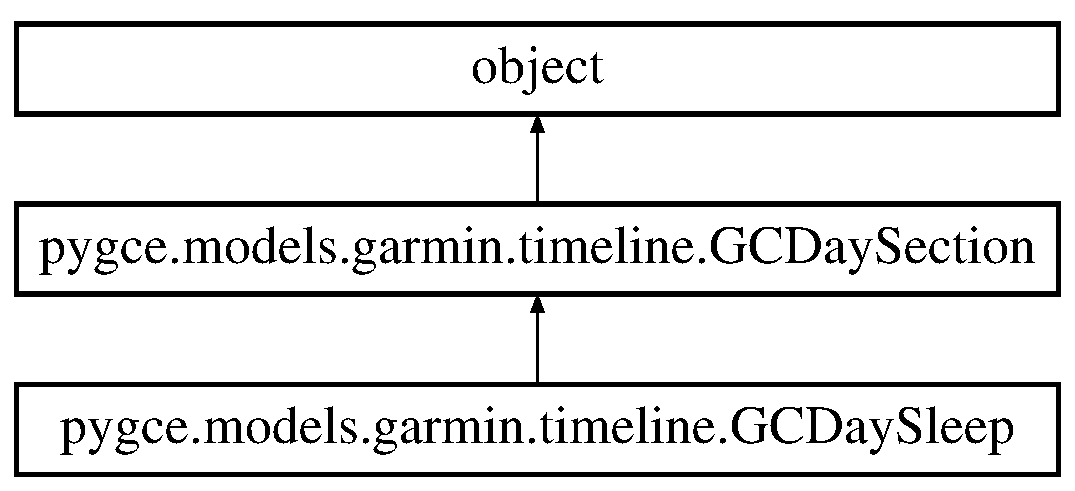
\includegraphics[height=2.000000cm]{classpygce_1_1models_1_1garmin_1_1timeline_1_1_g_c_day_sleep}
\end{center}
\end{figure}
\subsection*{Public Member Functions}
\begin{DoxyCompactItemize}
\item 
def \hyperlink{classpygce_1_1models_1_1garmin_1_1timeline_1_1_g_c_day_sleep_a58d1e0c8797955f8d88f1e662dc9ec76}{\+\_\+\+\_\+init\+\_\+\+\_\+} (self, raw\+\_\+html)
\item 
def \hyperlink{classpygce_1_1models_1_1garmin_1_1timeline_1_1_g_c_day_sleep_ad2906beca69f2678a5fb5fc619136039}{parse} (self)
\item 
def \hyperlink{classpygce_1_1models_1_1garmin_1_1timeline_1_1_g_c_day_sleep_aca0d551806aeaaaa7ca5ab55176a1677}{parse\+\_\+sleep\+\_\+totals} (self)
\item 
def \hyperlink{classpygce_1_1models_1_1garmin_1_1timeline_1_1_g_c_day_sleep_a1450b6f36eb2950df8d7b339191e0ac8}{parse\+\_\+bed\+\_\+time} (self)
\item 
def \hyperlink{classpygce_1_1models_1_1garmin_1_1timeline_1_1_g_c_day_sleep_af278bd0696f47ce317fb5e356fc6a438}{parse\+\_\+sleep\+\_\+times} (self)
\item 
def \hyperlink{classpygce_1_1models_1_1garmin_1_1timeline_1_1_g_c_day_sleep_a7ab65a28040de4131099b0479917eb75}{to\+\_\+dict} (self)
\end{DoxyCompactItemize}
\subsection*{Public Attributes}
\begin{DoxyCompactItemize}
\item 
\hyperlink{classpygce_1_1models_1_1garmin_1_1timeline_1_1_g_c_day_sleep_a4f8e3dadd2689156a80a21698b426e03}{night\+\_\+sleep\+\_\+time}
\item 
\hyperlink{classpygce_1_1models_1_1garmin_1_1timeline_1_1_g_c_day_sleep_af5aefe888d858cd929d598544802f2a8}{nap\+\_\+time}
\item 
\hyperlink{classpygce_1_1models_1_1garmin_1_1timeline_1_1_g_c_day_sleep_a4942fa038d25a7af4c0793da1b3abf86}{total\+\_\+sleep\+\_\+time}
\item 
\hyperlink{classpygce_1_1models_1_1garmin_1_1timeline_1_1_g_c_day_sleep_a25002c89e8687bc2a88ea5da386332cd}{bed\+\_\+time}
\item 
\hyperlink{classpygce_1_1models_1_1garmin_1_1timeline_1_1_g_c_day_sleep_abb2351f921e38ff370e1ad0822957553}{wake\+\_\+time}
\item 
\hyperlink{classpygce_1_1models_1_1garmin_1_1timeline_1_1_g_c_day_sleep_a95ebbbd000c531843a8a7fa7f8788f72}{deep\+\_\+sleep\+\_\+time}
\item 
\hyperlink{classpygce_1_1models_1_1garmin_1_1timeline_1_1_g_c_day_sleep_a49295ce80915e2012694a35edbf7ad7d}{light\+\_\+sleep\+\_\+time}
\item 
\hyperlink{classpygce_1_1models_1_1garmin_1_1timeline_1_1_g_c_day_sleep_aefd01be519ebb8192b0887941b66eda0}{awake\+\_\+sleep\+\_\+time}
\end{DoxyCompactItemize}


\subsection{Detailed Description}
\begin{DoxyVerb}Standard activity in the Garmin Connect timeline of day.
Common features are total, deep total, light total, awake total
\end{DoxyVerb}
 

Definition at line 258 of file timeline.\+py.



\subsection{Constructor \& Destructor Documentation}
\mbox{\Hypertarget{classpygce_1_1models_1_1garmin_1_1timeline_1_1_g_c_day_sleep_a58d1e0c8797955f8d88f1e662dc9ec76}\label{classpygce_1_1models_1_1garmin_1_1timeline_1_1_g_c_day_sleep_a58d1e0c8797955f8d88f1e662dc9ec76}} 
\index{pygce\+::models\+::garmin\+::timeline\+::\+G\+C\+Day\+Sleep@{pygce\+::models\+::garmin\+::timeline\+::\+G\+C\+Day\+Sleep}!\+\_\+\+\_\+init\+\_\+\+\_\+@{\+\_\+\+\_\+init\+\_\+\+\_\+}}
\index{\+\_\+\+\_\+init\+\_\+\+\_\+@{\+\_\+\+\_\+init\+\_\+\+\_\+}!pygce\+::models\+::garmin\+::timeline\+::\+G\+C\+Day\+Sleep@{pygce\+::models\+::garmin\+::timeline\+::\+G\+C\+Day\+Sleep}}
\subsubsection{\texorpdfstring{\+\_\+\+\_\+init\+\_\+\+\_\+()}{\_\_init\_\_()}}
{\footnotesize\ttfamily def pygce.\+models.\+garmin.\+timeline.\+G\+C\+Day\+Sleep.\+\_\+\+\_\+init\+\_\+\+\_\+ (\begin{DoxyParamCaption}\item[{}]{self,  }\item[{}]{raw\+\_\+html }\end{DoxyParamCaption})}

\begin{DoxyVerb}:param raw_html: str
    HTML source snippet with information about section
\end{DoxyVerb}
 

Definition at line 264 of file timeline.\+py.



\subsection{Member Function Documentation}
\mbox{\Hypertarget{classpygce_1_1models_1_1garmin_1_1timeline_1_1_g_c_day_sleep_ad2906beca69f2678a5fb5fc619136039}\label{classpygce_1_1models_1_1garmin_1_1timeline_1_1_g_c_day_sleep_ad2906beca69f2678a5fb5fc619136039}} 
\index{pygce\+::models\+::garmin\+::timeline\+::\+G\+C\+Day\+Sleep@{pygce\+::models\+::garmin\+::timeline\+::\+G\+C\+Day\+Sleep}!parse@{parse}}
\index{parse@{parse}!pygce\+::models\+::garmin\+::timeline\+::\+G\+C\+Day\+Sleep@{pygce\+::models\+::garmin\+::timeline\+::\+G\+C\+Day\+Sleep}}
\subsubsection{\texorpdfstring{parse()}{parse()}}
{\footnotesize\ttfamily def pygce.\+models.\+garmin.\+timeline.\+G\+C\+Day\+Sleep.\+parse (\begin{DoxyParamCaption}\item[{}]{self }\end{DoxyParamCaption})}



Definition at line 281 of file timeline.\+py.

\mbox{\Hypertarget{classpygce_1_1models_1_1garmin_1_1timeline_1_1_g_c_day_sleep_a1450b6f36eb2950df8d7b339191e0ac8}\label{classpygce_1_1models_1_1garmin_1_1timeline_1_1_g_c_day_sleep_a1450b6f36eb2950df8d7b339191e0ac8}} 
\index{pygce\+::models\+::garmin\+::timeline\+::\+G\+C\+Day\+Sleep@{pygce\+::models\+::garmin\+::timeline\+::\+G\+C\+Day\+Sleep}!parse\+\_\+bed\+\_\+time@{parse\+\_\+bed\+\_\+time}}
\index{parse\+\_\+bed\+\_\+time@{parse\+\_\+bed\+\_\+time}!pygce\+::models\+::garmin\+::timeline\+::\+G\+C\+Day\+Sleep@{pygce\+::models\+::garmin\+::timeline\+::\+G\+C\+Day\+Sleep}}
\subsubsection{\texorpdfstring{parse\+\_\+bed\+\_\+time()}{parse\_bed\_time()}}
{\footnotesize\ttfamily def pygce.\+models.\+garmin.\+timeline.\+G\+C\+Day\+Sleep.\+parse\+\_\+bed\+\_\+time (\begin{DoxyParamCaption}\item[{}]{self }\end{DoxyParamCaption})}

\begin{DoxyVerb}:return: void
    Finds hour start/end sleep
\end{DoxyVerb}
 

Definition at line 311 of file timeline.\+py.

\mbox{\Hypertarget{classpygce_1_1models_1_1garmin_1_1timeline_1_1_g_c_day_sleep_af278bd0696f47ce317fb5e356fc6a438}\label{classpygce_1_1models_1_1garmin_1_1timeline_1_1_g_c_day_sleep_af278bd0696f47ce317fb5e356fc6a438}} 
\index{pygce\+::models\+::garmin\+::timeline\+::\+G\+C\+Day\+Sleep@{pygce\+::models\+::garmin\+::timeline\+::\+G\+C\+Day\+Sleep}!parse\+\_\+sleep\+\_\+times@{parse\+\_\+sleep\+\_\+times}}
\index{parse\+\_\+sleep\+\_\+times@{parse\+\_\+sleep\+\_\+times}!pygce\+::models\+::garmin\+::timeline\+::\+G\+C\+Day\+Sleep@{pygce\+::models\+::garmin\+::timeline\+::\+G\+C\+Day\+Sleep}}
\subsubsection{\texorpdfstring{parse\+\_\+sleep\+\_\+times()}{parse\_sleep\_times()}}
{\footnotesize\ttfamily def pygce.\+models.\+garmin.\+timeline.\+G\+C\+Day\+Sleep.\+parse\+\_\+sleep\+\_\+times (\begin{DoxyParamCaption}\item[{}]{self }\end{DoxyParamCaption})}

\begin{DoxyVerb}:return: void
    Finds deep/light/awake sleep times
\end{DoxyVerb}
 

Definition at line 326 of file timeline.\+py.

\mbox{\Hypertarget{classpygce_1_1models_1_1garmin_1_1timeline_1_1_g_c_day_sleep_aca0d551806aeaaaa7ca5ab55176a1677}\label{classpygce_1_1models_1_1garmin_1_1timeline_1_1_g_c_day_sleep_aca0d551806aeaaaa7ca5ab55176a1677}} 
\index{pygce\+::models\+::garmin\+::timeline\+::\+G\+C\+Day\+Sleep@{pygce\+::models\+::garmin\+::timeline\+::\+G\+C\+Day\+Sleep}!parse\+\_\+sleep\+\_\+totals@{parse\+\_\+sleep\+\_\+totals}}
\index{parse\+\_\+sleep\+\_\+totals@{parse\+\_\+sleep\+\_\+totals}!pygce\+::models\+::garmin\+::timeline\+::\+G\+C\+Day\+Sleep@{pygce\+::models\+::garmin\+::timeline\+::\+G\+C\+Day\+Sleep}}
\subsubsection{\texorpdfstring{parse\+\_\+sleep\+\_\+totals()}{parse\_sleep\_totals()}}
{\footnotesize\ttfamily def pygce.\+models.\+garmin.\+timeline.\+G\+C\+Day\+Sleep.\+parse\+\_\+sleep\+\_\+totals (\begin{DoxyParamCaption}\item[{}]{self }\end{DoxyParamCaption})}

\begin{DoxyVerb}:return: void
    Finds value of night/nap/total sleep times
\end{DoxyVerb}
 

Definition at line 297 of file timeline.\+py.

\mbox{\Hypertarget{classpygce_1_1models_1_1garmin_1_1timeline_1_1_g_c_day_sleep_a7ab65a28040de4131099b0479917eb75}\label{classpygce_1_1models_1_1garmin_1_1timeline_1_1_g_c_day_sleep_a7ab65a28040de4131099b0479917eb75}} 
\index{pygce\+::models\+::garmin\+::timeline\+::\+G\+C\+Day\+Sleep@{pygce\+::models\+::garmin\+::timeline\+::\+G\+C\+Day\+Sleep}!to\+\_\+dict@{to\+\_\+dict}}
\index{to\+\_\+dict@{to\+\_\+dict}!pygce\+::models\+::garmin\+::timeline\+::\+G\+C\+Day\+Sleep@{pygce\+::models\+::garmin\+::timeline\+::\+G\+C\+Day\+Sleep}}
\subsubsection{\texorpdfstring{to\+\_\+dict()}{to\_dict()}}
{\footnotesize\ttfamily def pygce.\+models.\+garmin.\+timeline.\+G\+C\+Day\+Sleep.\+to\+\_\+dict (\begin{DoxyParamCaption}\item[{}]{self }\end{DoxyParamCaption})}



Definition at line 351 of file timeline.\+py.



\subsection{Member Data Documentation}
\mbox{\Hypertarget{classpygce_1_1models_1_1garmin_1_1timeline_1_1_g_c_day_sleep_aefd01be519ebb8192b0887941b66eda0}\label{classpygce_1_1models_1_1garmin_1_1timeline_1_1_g_c_day_sleep_aefd01be519ebb8192b0887941b66eda0}} 
\index{pygce\+::models\+::garmin\+::timeline\+::\+G\+C\+Day\+Sleep@{pygce\+::models\+::garmin\+::timeline\+::\+G\+C\+Day\+Sleep}!awake\+\_\+sleep\+\_\+time@{awake\+\_\+sleep\+\_\+time}}
\index{awake\+\_\+sleep\+\_\+time@{awake\+\_\+sleep\+\_\+time}!pygce\+::models\+::garmin\+::timeline\+::\+G\+C\+Day\+Sleep@{pygce\+::models\+::garmin\+::timeline\+::\+G\+C\+Day\+Sleep}}
\subsubsection{\texorpdfstring{awake\+\_\+sleep\+\_\+time}{awake\_sleep\_time}}
{\footnotesize\ttfamily pygce.\+models.\+garmin.\+timeline.\+G\+C\+Day\+Sleep.\+awake\+\_\+sleep\+\_\+time}



Definition at line 279 of file timeline.\+py.

\mbox{\Hypertarget{classpygce_1_1models_1_1garmin_1_1timeline_1_1_g_c_day_sleep_a25002c89e8687bc2a88ea5da386332cd}\label{classpygce_1_1models_1_1garmin_1_1timeline_1_1_g_c_day_sleep_a25002c89e8687bc2a88ea5da386332cd}} 
\index{pygce\+::models\+::garmin\+::timeline\+::\+G\+C\+Day\+Sleep@{pygce\+::models\+::garmin\+::timeline\+::\+G\+C\+Day\+Sleep}!bed\+\_\+time@{bed\+\_\+time}}
\index{bed\+\_\+time@{bed\+\_\+time}!pygce\+::models\+::garmin\+::timeline\+::\+G\+C\+Day\+Sleep@{pygce\+::models\+::garmin\+::timeline\+::\+G\+C\+Day\+Sleep}}
\subsubsection{\texorpdfstring{bed\+\_\+time}{bed\_time}}
{\footnotesize\ttfamily pygce.\+models.\+garmin.\+timeline.\+G\+C\+Day\+Sleep.\+bed\+\_\+time}



Definition at line 275 of file timeline.\+py.

\mbox{\Hypertarget{classpygce_1_1models_1_1garmin_1_1timeline_1_1_g_c_day_sleep_a95ebbbd000c531843a8a7fa7f8788f72}\label{classpygce_1_1models_1_1garmin_1_1timeline_1_1_g_c_day_sleep_a95ebbbd000c531843a8a7fa7f8788f72}} 
\index{pygce\+::models\+::garmin\+::timeline\+::\+G\+C\+Day\+Sleep@{pygce\+::models\+::garmin\+::timeline\+::\+G\+C\+Day\+Sleep}!deep\+\_\+sleep\+\_\+time@{deep\+\_\+sleep\+\_\+time}}
\index{deep\+\_\+sleep\+\_\+time@{deep\+\_\+sleep\+\_\+time}!pygce\+::models\+::garmin\+::timeline\+::\+G\+C\+Day\+Sleep@{pygce\+::models\+::garmin\+::timeline\+::\+G\+C\+Day\+Sleep}}
\subsubsection{\texorpdfstring{deep\+\_\+sleep\+\_\+time}{deep\_sleep\_time}}
{\footnotesize\ttfamily pygce.\+models.\+garmin.\+timeline.\+G\+C\+Day\+Sleep.\+deep\+\_\+sleep\+\_\+time}



Definition at line 277 of file timeline.\+py.

\mbox{\Hypertarget{classpygce_1_1models_1_1garmin_1_1timeline_1_1_g_c_day_sleep_a49295ce80915e2012694a35edbf7ad7d}\label{classpygce_1_1models_1_1garmin_1_1timeline_1_1_g_c_day_sleep_a49295ce80915e2012694a35edbf7ad7d}} 
\index{pygce\+::models\+::garmin\+::timeline\+::\+G\+C\+Day\+Sleep@{pygce\+::models\+::garmin\+::timeline\+::\+G\+C\+Day\+Sleep}!light\+\_\+sleep\+\_\+time@{light\+\_\+sleep\+\_\+time}}
\index{light\+\_\+sleep\+\_\+time@{light\+\_\+sleep\+\_\+time}!pygce\+::models\+::garmin\+::timeline\+::\+G\+C\+Day\+Sleep@{pygce\+::models\+::garmin\+::timeline\+::\+G\+C\+Day\+Sleep}}
\subsubsection{\texorpdfstring{light\+\_\+sleep\+\_\+time}{light\_sleep\_time}}
{\footnotesize\ttfamily pygce.\+models.\+garmin.\+timeline.\+G\+C\+Day\+Sleep.\+light\+\_\+sleep\+\_\+time}



Definition at line 278 of file timeline.\+py.

\mbox{\Hypertarget{classpygce_1_1models_1_1garmin_1_1timeline_1_1_g_c_day_sleep_af5aefe888d858cd929d598544802f2a8}\label{classpygce_1_1models_1_1garmin_1_1timeline_1_1_g_c_day_sleep_af5aefe888d858cd929d598544802f2a8}} 
\index{pygce\+::models\+::garmin\+::timeline\+::\+G\+C\+Day\+Sleep@{pygce\+::models\+::garmin\+::timeline\+::\+G\+C\+Day\+Sleep}!nap\+\_\+time@{nap\+\_\+time}}
\index{nap\+\_\+time@{nap\+\_\+time}!pygce\+::models\+::garmin\+::timeline\+::\+G\+C\+Day\+Sleep@{pygce\+::models\+::garmin\+::timeline\+::\+G\+C\+Day\+Sleep}}
\subsubsection{\texorpdfstring{nap\+\_\+time}{nap\_time}}
{\footnotesize\ttfamily pygce.\+models.\+garmin.\+timeline.\+G\+C\+Day\+Sleep.\+nap\+\_\+time}



Definition at line 273 of file timeline.\+py.

\mbox{\Hypertarget{classpygce_1_1models_1_1garmin_1_1timeline_1_1_g_c_day_sleep_a4f8e3dadd2689156a80a21698b426e03}\label{classpygce_1_1models_1_1garmin_1_1timeline_1_1_g_c_day_sleep_a4f8e3dadd2689156a80a21698b426e03}} 
\index{pygce\+::models\+::garmin\+::timeline\+::\+G\+C\+Day\+Sleep@{pygce\+::models\+::garmin\+::timeline\+::\+G\+C\+Day\+Sleep}!night\+\_\+sleep\+\_\+time@{night\+\_\+sleep\+\_\+time}}
\index{night\+\_\+sleep\+\_\+time@{night\+\_\+sleep\+\_\+time}!pygce\+::models\+::garmin\+::timeline\+::\+G\+C\+Day\+Sleep@{pygce\+::models\+::garmin\+::timeline\+::\+G\+C\+Day\+Sleep}}
\subsubsection{\texorpdfstring{night\+\_\+sleep\+\_\+time}{night\_sleep\_time}}
{\footnotesize\ttfamily pygce.\+models.\+garmin.\+timeline.\+G\+C\+Day\+Sleep.\+night\+\_\+sleep\+\_\+time}



Definition at line 272 of file timeline.\+py.

\mbox{\Hypertarget{classpygce_1_1models_1_1garmin_1_1timeline_1_1_g_c_day_sleep_a4942fa038d25a7af4c0793da1b3abf86}\label{classpygce_1_1models_1_1garmin_1_1timeline_1_1_g_c_day_sleep_a4942fa038d25a7af4c0793da1b3abf86}} 
\index{pygce\+::models\+::garmin\+::timeline\+::\+G\+C\+Day\+Sleep@{pygce\+::models\+::garmin\+::timeline\+::\+G\+C\+Day\+Sleep}!total\+\_\+sleep\+\_\+time@{total\+\_\+sleep\+\_\+time}}
\index{total\+\_\+sleep\+\_\+time@{total\+\_\+sleep\+\_\+time}!pygce\+::models\+::garmin\+::timeline\+::\+G\+C\+Day\+Sleep@{pygce\+::models\+::garmin\+::timeline\+::\+G\+C\+Day\+Sleep}}
\subsubsection{\texorpdfstring{total\+\_\+sleep\+\_\+time}{total\_sleep\_time}}
{\footnotesize\ttfamily pygce.\+models.\+garmin.\+timeline.\+G\+C\+Day\+Sleep.\+total\+\_\+sleep\+\_\+time}



Definition at line 274 of file timeline.\+py.

\mbox{\Hypertarget{classpygce_1_1models_1_1garmin_1_1timeline_1_1_g_c_day_sleep_abb2351f921e38ff370e1ad0822957553}\label{classpygce_1_1models_1_1garmin_1_1timeline_1_1_g_c_day_sleep_abb2351f921e38ff370e1ad0822957553}} 
\index{pygce\+::models\+::garmin\+::timeline\+::\+G\+C\+Day\+Sleep@{pygce\+::models\+::garmin\+::timeline\+::\+G\+C\+Day\+Sleep}!wake\+\_\+time@{wake\+\_\+time}}
\index{wake\+\_\+time@{wake\+\_\+time}!pygce\+::models\+::garmin\+::timeline\+::\+G\+C\+Day\+Sleep@{pygce\+::models\+::garmin\+::timeline\+::\+G\+C\+Day\+Sleep}}
\subsubsection{\texorpdfstring{wake\+\_\+time}{wake\_time}}
{\footnotesize\ttfamily pygce.\+models.\+garmin.\+timeline.\+G\+C\+Day\+Sleep.\+wake\+\_\+time}



Definition at line 276 of file timeline.\+py.



The documentation for this class was generated from the following file\+:\begin{DoxyCompactItemize}
\item 
/home/stefano/\+Coding/\+Python/\+\_\+projects/pygce/pygce/models/garmin/\hyperlink{timeline_8py}{timeline.\+py}\end{DoxyCompactItemize}

\hypertarget{classpygce_1_1models_1_1garmin_1_1timeline_1_1_g_c_day_steps}{}\section{pygce.\+models.\+garmin.\+timeline.\+G\+C\+Day\+Steps Class Reference}
\label{classpygce_1_1models_1_1garmin_1_1timeline_1_1_g_c_day_steps}\index{pygce.\+models.\+garmin.\+timeline.\+G\+C\+Day\+Steps@{pygce.\+models.\+garmin.\+timeline.\+G\+C\+Day\+Steps}}
Inheritance diagram for pygce.\+models.\+garmin.\+timeline.\+G\+C\+Day\+Steps\+:\begin{figure}[H]
\begin{center}
\leavevmode
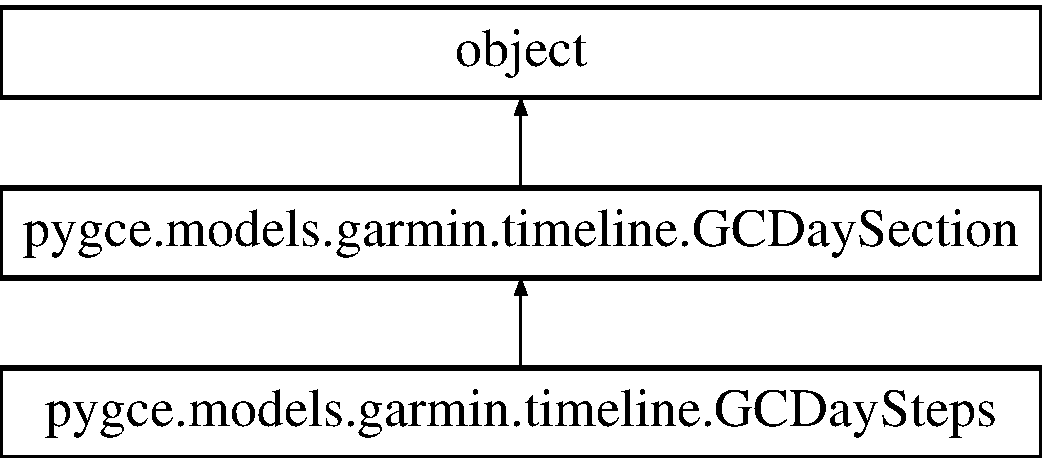
\includegraphics[height=3.000000cm]{classpygce_1_1models_1_1garmin_1_1timeline_1_1_g_c_day_steps}
\end{center}
\end{figure}
\subsection*{Public Member Functions}
\begin{DoxyCompactItemize}
\item 
def \hyperlink{classpygce_1_1models_1_1garmin_1_1timeline_1_1_g_c_day_steps_a0b8cc0a273e2a35d5326b3e06c39e4a1}{\+\_\+\+\_\+init\+\_\+\+\_\+} (self, raw\+\_\+html)
\item 
def \hyperlink{classpygce_1_1models_1_1garmin_1_1timeline_1_1_g_c_day_steps_ae75ac9895d92ca73d95e451d92454f4e}{parse} (self)
\item 
def \hyperlink{classpygce_1_1models_1_1garmin_1_1timeline_1_1_g_c_day_steps_ab5fa162419e53f44464d5e0ce5d4a31f}{parse\+\_\+steps\+\_\+count} (self)
\item 
def \hyperlink{classpygce_1_1models_1_1garmin_1_1timeline_1_1_g_c_day_steps_a994d3d53c4f1eaa9729349d043e010f7}{parse\+\_\+steps\+\_\+stats} (self)
\item 
def \hyperlink{classpygce_1_1models_1_1garmin_1_1timeline_1_1_g_c_day_steps_ae464eda48e08d995c704199a73055e95}{to\+\_\+dict} (self)
\end{DoxyCompactItemize}
\subsection*{Public Attributes}
\begin{DoxyCompactItemize}
\item 
\hyperlink{classpygce_1_1models_1_1garmin_1_1timeline_1_1_g_c_day_steps_accaf8fa0f07a44164f5e2ee3a4c5fca7}{total}
\item 
\hyperlink{classpygce_1_1models_1_1garmin_1_1timeline_1_1_g_c_day_steps_a60204221cb98c4d801fa4265c2dbf5ef}{goal}
\item 
\hyperlink{classpygce_1_1models_1_1garmin_1_1timeline_1_1_g_c_day_steps_a598091ff91043c28a7bb4711f861ff71}{avg}
\item 
\hyperlink{classpygce_1_1models_1_1garmin_1_1timeline_1_1_g_c_day_steps_a3fe1eac606ace83c095f9c376d1e09ba}{distance}
\end{DoxyCompactItemize}


\subsection{Detailed Description}
\begin{DoxyVerb}Standard activity in the Garmin Connect timeline of day.
Common features are total, goal, distance, avg daily
\end{DoxyVerb}
 

Definition at line 139 of file timeline.\+py.



\subsection{Constructor \& Destructor Documentation}
\mbox{\Hypertarget{classpygce_1_1models_1_1garmin_1_1timeline_1_1_g_c_day_steps_a0b8cc0a273e2a35d5326b3e06c39e4a1}\label{classpygce_1_1models_1_1garmin_1_1timeline_1_1_g_c_day_steps_a0b8cc0a273e2a35d5326b3e06c39e4a1}} 
\index{pygce\+::models\+::garmin\+::timeline\+::\+G\+C\+Day\+Steps@{pygce\+::models\+::garmin\+::timeline\+::\+G\+C\+Day\+Steps}!\+\_\+\+\_\+init\+\_\+\+\_\+@{\+\_\+\+\_\+init\+\_\+\+\_\+}}
\index{\+\_\+\+\_\+init\+\_\+\+\_\+@{\+\_\+\+\_\+init\+\_\+\+\_\+}!pygce\+::models\+::garmin\+::timeline\+::\+G\+C\+Day\+Steps@{pygce\+::models\+::garmin\+::timeline\+::\+G\+C\+Day\+Steps}}
\subsubsection{\texorpdfstring{\+\_\+\+\_\+init\+\_\+\+\_\+()}{\_\_init\_\_()}}
{\footnotesize\ttfamily def pygce.\+models.\+garmin.\+timeline.\+G\+C\+Day\+Steps.\+\_\+\+\_\+init\+\_\+\+\_\+ (\begin{DoxyParamCaption}\item[{}]{self,  }\item[{}]{raw\+\_\+html }\end{DoxyParamCaption})}

\begin{DoxyVerb}:param raw_html: str
    HTML source snippet with information about section
\end{DoxyVerb}
 

Definition at line 145 of file timeline.\+py.



\subsection{Member Function Documentation}
\mbox{\Hypertarget{classpygce_1_1models_1_1garmin_1_1timeline_1_1_g_c_day_steps_ae75ac9895d92ca73d95e451d92454f4e}\label{classpygce_1_1models_1_1garmin_1_1timeline_1_1_g_c_day_steps_ae75ac9895d92ca73d95e451d92454f4e}} 
\index{pygce\+::models\+::garmin\+::timeline\+::\+G\+C\+Day\+Steps@{pygce\+::models\+::garmin\+::timeline\+::\+G\+C\+Day\+Steps}!parse@{parse}}
\index{parse@{parse}!pygce\+::models\+::garmin\+::timeline\+::\+G\+C\+Day\+Steps@{pygce\+::models\+::garmin\+::timeline\+::\+G\+C\+Day\+Steps}}
\subsubsection{\texorpdfstring{parse()}{parse()}}
{\footnotesize\ttfamily def pygce.\+models.\+garmin.\+timeline.\+G\+C\+Day\+Steps.\+parse (\begin{DoxyParamCaption}\item[{}]{self }\end{DoxyParamCaption})}



Definition at line 158 of file timeline.\+py.

\mbox{\Hypertarget{classpygce_1_1models_1_1garmin_1_1timeline_1_1_g_c_day_steps_ab5fa162419e53f44464d5e0ce5d4a31f}\label{classpygce_1_1models_1_1garmin_1_1timeline_1_1_g_c_day_steps_ab5fa162419e53f44464d5e0ce5d4a31f}} 
\index{pygce\+::models\+::garmin\+::timeline\+::\+G\+C\+Day\+Steps@{pygce\+::models\+::garmin\+::timeline\+::\+G\+C\+Day\+Steps}!parse\+\_\+steps\+\_\+count@{parse\+\_\+steps\+\_\+count}}
\index{parse\+\_\+steps\+\_\+count@{parse\+\_\+steps\+\_\+count}!pygce\+::models\+::garmin\+::timeline\+::\+G\+C\+Day\+Steps@{pygce\+::models\+::garmin\+::timeline\+::\+G\+C\+Day\+Steps}}
\subsubsection{\texorpdfstring{parse\+\_\+steps\+\_\+count()}{parse\_steps\_count()}}
{\footnotesize\ttfamily def pygce.\+models.\+garmin.\+timeline.\+G\+C\+Day\+Steps.\+parse\+\_\+steps\+\_\+count (\begin{DoxyParamCaption}\item[{}]{self }\end{DoxyParamCaption})}

\begin{DoxyVerb}:return: void
    Parses HTML source and finds goal and daily steps
\end{DoxyVerb}
 

Definition at line 162 of file timeline.\+py.

\mbox{\Hypertarget{classpygce_1_1models_1_1garmin_1_1timeline_1_1_g_c_day_steps_a994d3d53c4f1eaa9729349d043e010f7}\label{classpygce_1_1models_1_1garmin_1_1timeline_1_1_g_c_day_steps_a994d3d53c4f1eaa9729349d043e010f7}} 
\index{pygce\+::models\+::garmin\+::timeline\+::\+G\+C\+Day\+Steps@{pygce\+::models\+::garmin\+::timeline\+::\+G\+C\+Day\+Steps}!parse\+\_\+steps\+\_\+stats@{parse\+\_\+steps\+\_\+stats}}
\index{parse\+\_\+steps\+\_\+stats@{parse\+\_\+steps\+\_\+stats}!pygce\+::models\+::garmin\+::timeline\+::\+G\+C\+Day\+Steps@{pygce\+::models\+::garmin\+::timeline\+::\+G\+C\+Day\+Steps}}
\subsubsection{\texorpdfstring{parse\+\_\+steps\+\_\+stats()}{parse\_steps\_stats()}}
{\footnotesize\ttfamily def pygce.\+models.\+garmin.\+timeline.\+G\+C\+Day\+Steps.\+parse\+\_\+steps\+\_\+stats (\begin{DoxyParamCaption}\item[{}]{self }\end{DoxyParamCaption})}

\begin{DoxyVerb}:return: void
    Parses HTML source and finds daily distance and avg daily steps
\end{DoxyVerb}
 

Definition at line 181 of file timeline.\+py.

\mbox{\Hypertarget{classpygce_1_1models_1_1garmin_1_1timeline_1_1_g_c_day_steps_ae464eda48e08d995c704199a73055e95}\label{classpygce_1_1models_1_1garmin_1_1timeline_1_1_g_c_day_steps_ae464eda48e08d995c704199a73055e95}} 
\index{pygce\+::models\+::garmin\+::timeline\+::\+G\+C\+Day\+Steps@{pygce\+::models\+::garmin\+::timeline\+::\+G\+C\+Day\+Steps}!to\+\_\+dict@{to\+\_\+dict}}
\index{to\+\_\+dict@{to\+\_\+dict}!pygce\+::models\+::garmin\+::timeline\+::\+G\+C\+Day\+Steps@{pygce\+::models\+::garmin\+::timeline\+::\+G\+C\+Day\+Steps}}
\subsubsection{\texorpdfstring{to\+\_\+dict()}{to\_dict()}}
{\footnotesize\ttfamily def pygce.\+models.\+garmin.\+timeline.\+G\+C\+Day\+Steps.\+to\+\_\+dict (\begin{DoxyParamCaption}\item[{}]{self }\end{DoxyParamCaption})}



Definition at line 195 of file timeline.\+py.



\subsection{Member Data Documentation}
\mbox{\Hypertarget{classpygce_1_1models_1_1garmin_1_1timeline_1_1_g_c_day_steps_a598091ff91043c28a7bb4711f861ff71}\label{classpygce_1_1models_1_1garmin_1_1timeline_1_1_g_c_day_steps_a598091ff91043c28a7bb4711f861ff71}} 
\index{pygce\+::models\+::garmin\+::timeline\+::\+G\+C\+Day\+Steps@{pygce\+::models\+::garmin\+::timeline\+::\+G\+C\+Day\+Steps}!avg@{avg}}
\index{avg@{avg}!pygce\+::models\+::garmin\+::timeline\+::\+G\+C\+Day\+Steps@{pygce\+::models\+::garmin\+::timeline\+::\+G\+C\+Day\+Steps}}
\subsubsection{\texorpdfstring{avg}{avg}}
{\footnotesize\ttfamily pygce.\+models.\+garmin.\+timeline.\+G\+C\+Day\+Steps.\+avg}



Definition at line 155 of file timeline.\+py.

\mbox{\Hypertarget{classpygce_1_1models_1_1garmin_1_1timeline_1_1_g_c_day_steps_a3fe1eac606ace83c095f9c376d1e09ba}\label{classpygce_1_1models_1_1garmin_1_1timeline_1_1_g_c_day_steps_a3fe1eac606ace83c095f9c376d1e09ba}} 
\index{pygce\+::models\+::garmin\+::timeline\+::\+G\+C\+Day\+Steps@{pygce\+::models\+::garmin\+::timeline\+::\+G\+C\+Day\+Steps}!distance@{distance}}
\index{distance@{distance}!pygce\+::models\+::garmin\+::timeline\+::\+G\+C\+Day\+Steps@{pygce\+::models\+::garmin\+::timeline\+::\+G\+C\+Day\+Steps}}
\subsubsection{\texorpdfstring{distance}{distance}}
{\footnotesize\ttfamily pygce.\+models.\+garmin.\+timeline.\+G\+C\+Day\+Steps.\+distance}



Definition at line 156 of file timeline.\+py.

\mbox{\Hypertarget{classpygce_1_1models_1_1garmin_1_1timeline_1_1_g_c_day_steps_a60204221cb98c4d801fa4265c2dbf5ef}\label{classpygce_1_1models_1_1garmin_1_1timeline_1_1_g_c_day_steps_a60204221cb98c4d801fa4265c2dbf5ef}} 
\index{pygce\+::models\+::garmin\+::timeline\+::\+G\+C\+Day\+Steps@{pygce\+::models\+::garmin\+::timeline\+::\+G\+C\+Day\+Steps}!goal@{goal}}
\index{goal@{goal}!pygce\+::models\+::garmin\+::timeline\+::\+G\+C\+Day\+Steps@{pygce\+::models\+::garmin\+::timeline\+::\+G\+C\+Day\+Steps}}
\subsubsection{\texorpdfstring{goal}{goal}}
{\footnotesize\ttfamily pygce.\+models.\+garmin.\+timeline.\+G\+C\+Day\+Steps.\+goal}



Definition at line 154 of file timeline.\+py.

\mbox{\Hypertarget{classpygce_1_1models_1_1garmin_1_1timeline_1_1_g_c_day_steps_accaf8fa0f07a44164f5e2ee3a4c5fca7}\label{classpygce_1_1models_1_1garmin_1_1timeline_1_1_g_c_day_steps_accaf8fa0f07a44164f5e2ee3a4c5fca7}} 
\index{pygce\+::models\+::garmin\+::timeline\+::\+G\+C\+Day\+Steps@{pygce\+::models\+::garmin\+::timeline\+::\+G\+C\+Day\+Steps}!total@{total}}
\index{total@{total}!pygce\+::models\+::garmin\+::timeline\+::\+G\+C\+Day\+Steps@{pygce\+::models\+::garmin\+::timeline\+::\+G\+C\+Day\+Steps}}
\subsubsection{\texorpdfstring{total}{total}}
{\footnotesize\ttfamily pygce.\+models.\+garmin.\+timeline.\+G\+C\+Day\+Steps.\+total}



Definition at line 153 of file timeline.\+py.



The documentation for this class was generated from the following file\+:\begin{DoxyCompactItemize}
\item 
/home/stefano/\+Coding/\+Python/projects/pygce/pygce/models/garmin/\hyperlink{timeline_8py}{timeline.\+py}\end{DoxyCompactItemize}

\hypertarget{classpygce_1_1models_1_1garmin_1_1timeline_1_1_g_c_day_summary}{}\section{pygce.\+models.\+garmin.\+timeline.\+G\+C\+Day\+Summary Class Reference}
\label{classpygce_1_1models_1_1garmin_1_1timeline_1_1_g_c_day_summary}\index{pygce.\+models.\+garmin.\+timeline.\+G\+C\+Day\+Summary@{pygce.\+models.\+garmin.\+timeline.\+G\+C\+Day\+Summary}}
Inheritance diagram for pygce.\+models.\+garmin.\+timeline.\+G\+C\+Day\+Summary\+:\begin{figure}[H]
\begin{center}
\leavevmode
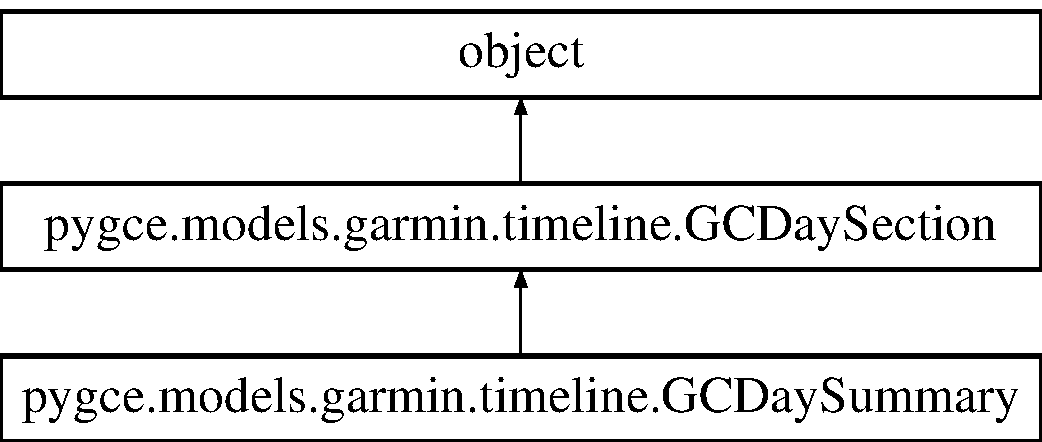
\includegraphics[height=3.000000cm]{classpygce_1_1models_1_1garmin_1_1timeline_1_1_g_c_day_summary}
\end{center}
\end{figure}
\subsection*{Public Member Functions}
\begin{DoxyCompactItemize}
\item 
def \hyperlink{classpygce_1_1models_1_1garmin_1_1timeline_1_1_g_c_day_summary_a9af14ec017803981a9b6047877d92be7}{\+\_\+\+\_\+init\+\_\+\+\_\+} (self, raw\+\_\+html)
\item 
def \hyperlink{classpygce_1_1models_1_1garmin_1_1timeline_1_1_g_c_day_summary_ab7b302fdc532d60ac846230bc0a28150}{parse} (self)
\item 
def \hyperlink{classpygce_1_1models_1_1garmin_1_1timeline_1_1_g_c_day_summary_a6b4f9c47531f9a6ed2f82751153a6611}{parse\+\_\+likes} (self)
\item 
def \hyperlink{classpygce_1_1models_1_1garmin_1_1timeline_1_1_g_c_day_summary_adb9b8c1210354666d6a137d3e1cc50c4}{parse\+\_\+comment} (self)
\item 
def \hyperlink{classpygce_1_1models_1_1garmin_1_1timeline_1_1_g_c_day_summary_a96e573903735f0ed37698d79d43116f0}{parse\+\_\+kcal\+\_\+count} (self)
\item 
def \hyperlink{classpygce_1_1models_1_1garmin_1_1timeline_1_1_g_c_day_summary_a65d756c22031bee3eebcef9e1df1040b}{to\+\_\+dict} (self)
\end{DoxyCompactItemize}
\subsection*{Public Attributes}
\begin{DoxyCompactItemize}
\item 
\hyperlink{classpygce_1_1models_1_1garmin_1_1timeline_1_1_g_c_day_summary_a3fc863d92101994b0c2263b6f0cae4c4}{likes}
\item 
\hyperlink{classpygce_1_1models_1_1garmin_1_1timeline_1_1_g_c_day_summary_af38e9e07196f995d9e8551bb69940f3d}{comment}
\item 
\hyperlink{classpygce_1_1models_1_1garmin_1_1timeline_1_1_g_c_day_summary_a16ed8d554c0349a90d281cbd58608153}{kcal\+\_\+count}
\end{DoxyCompactItemize}


\subsection{Detailed Description}
\begin{DoxyVerb}Standard activity in the Garmin Connect timeline of day.
Common features are likes, comment, kcal
\end{DoxyVerb}
 

Definition at line 86 of file timeline.\+py.



\subsection{Constructor \& Destructor Documentation}
\index{pygce\+::models\+::garmin\+::timeline\+::\+G\+C\+Day\+Summary@{pygce\+::models\+::garmin\+::timeline\+::\+G\+C\+Day\+Summary}!\+\_\+\+\_\+init\+\_\+\+\_\+@{\+\_\+\+\_\+init\+\_\+\+\_\+}}
\index{\+\_\+\+\_\+init\+\_\+\+\_\+@{\+\_\+\+\_\+init\+\_\+\+\_\+}!pygce\+::models\+::garmin\+::timeline\+::\+G\+C\+Day\+Summary@{pygce\+::models\+::garmin\+::timeline\+::\+G\+C\+Day\+Summary}}
\subsubsection[{\texorpdfstring{\+\_\+\+\_\+init\+\_\+\+\_\+(self, raw\+\_\+html)}{__init__(self, raw_html)}}]{\setlength{\rightskip}{0pt plus 5cm}def pygce.\+models.\+garmin.\+timeline.\+G\+C\+Day\+Summary.\+\_\+\+\_\+init\+\_\+\+\_\+ (
\begin{DoxyParamCaption}
\item[{}]{self, }
\item[{}]{raw\+\_\+html}
\end{DoxyParamCaption}
)}\hypertarget{classpygce_1_1models_1_1garmin_1_1timeline_1_1_g_c_day_summary_a9af14ec017803981a9b6047877d92be7}{}\label{classpygce_1_1models_1_1garmin_1_1timeline_1_1_g_c_day_summary_a9af14ec017803981a9b6047877d92be7}
\begin{DoxyVerb}:param raw_html: str
    HTML source snippet with information about section
\end{DoxyVerb}
 

Definition at line 92 of file timeline.\+py.



\subsection{Member Function Documentation}
\index{pygce\+::models\+::garmin\+::timeline\+::\+G\+C\+Day\+Summary@{pygce\+::models\+::garmin\+::timeline\+::\+G\+C\+Day\+Summary}!parse@{parse}}
\index{parse@{parse}!pygce\+::models\+::garmin\+::timeline\+::\+G\+C\+Day\+Summary@{pygce\+::models\+::garmin\+::timeline\+::\+G\+C\+Day\+Summary}}
\subsubsection[{\texorpdfstring{parse(self)}{parse(self)}}]{\setlength{\rightskip}{0pt plus 5cm}def pygce.\+models.\+garmin.\+timeline.\+G\+C\+Day\+Summary.\+parse (
\begin{DoxyParamCaption}
\item[{}]{self}
\end{DoxyParamCaption}
)}\hypertarget{classpygce_1_1models_1_1garmin_1_1timeline_1_1_g_c_day_summary_ab7b302fdc532d60ac846230bc0a28150}{}\label{classpygce_1_1models_1_1garmin_1_1timeline_1_1_g_c_day_summary_ab7b302fdc532d60ac846230bc0a28150}


Definition at line 104 of file timeline.\+py.

\index{pygce\+::models\+::garmin\+::timeline\+::\+G\+C\+Day\+Summary@{pygce\+::models\+::garmin\+::timeline\+::\+G\+C\+Day\+Summary}!parse\+\_\+comment@{parse\+\_\+comment}}
\index{parse\+\_\+comment@{parse\+\_\+comment}!pygce\+::models\+::garmin\+::timeline\+::\+G\+C\+Day\+Summary@{pygce\+::models\+::garmin\+::timeline\+::\+G\+C\+Day\+Summary}}
\subsubsection[{\texorpdfstring{parse\+\_\+comment(self)}{parse_comment(self)}}]{\setlength{\rightskip}{0pt plus 5cm}def pygce.\+models.\+garmin.\+timeline.\+G\+C\+Day\+Summary.\+parse\+\_\+comment (
\begin{DoxyParamCaption}
\item[{}]{self}
\end{DoxyParamCaption}
)}\hypertarget{classpygce_1_1models_1_1garmin_1_1timeline_1_1_g_c_day_summary_adb9b8c1210354666d6a137d3e1cc50c4}{}\label{classpygce_1_1models_1_1garmin_1_1timeline_1_1_g_c_day_summary_adb9b8c1210354666d6a137d3e1cc50c4}
\begin{DoxyVerb}:return: void
    Finds comment value and stores value
\end{DoxyVerb}
 

Definition at line 120 of file timeline.\+py.

\index{pygce\+::models\+::garmin\+::timeline\+::\+G\+C\+Day\+Summary@{pygce\+::models\+::garmin\+::timeline\+::\+G\+C\+Day\+Summary}!parse\+\_\+kcal\+\_\+count@{parse\+\_\+kcal\+\_\+count}}
\index{parse\+\_\+kcal\+\_\+count@{parse\+\_\+kcal\+\_\+count}!pygce\+::models\+::garmin\+::timeline\+::\+G\+C\+Day\+Summary@{pygce\+::models\+::garmin\+::timeline\+::\+G\+C\+Day\+Summary}}
\subsubsection[{\texorpdfstring{parse\+\_\+kcal\+\_\+count(self)}{parse_kcal_count(self)}}]{\setlength{\rightskip}{0pt plus 5cm}def pygce.\+models.\+garmin.\+timeline.\+G\+C\+Day\+Summary.\+parse\+\_\+kcal\+\_\+count (
\begin{DoxyParamCaption}
\item[{}]{self}
\end{DoxyParamCaption}
)}\hypertarget{classpygce_1_1models_1_1garmin_1_1timeline_1_1_g_c_day_summary_a96e573903735f0ed37698d79d43116f0}{}\label{classpygce_1_1models_1_1garmin_1_1timeline_1_1_g_c_day_summary_a96e573903735f0ed37698d79d43116f0}
\begin{DoxyVerb}:return: void
    Finds kcal value and stores value
\end{DoxyVerb}
 

Definition at line 131 of file timeline.\+py.

\index{pygce\+::models\+::garmin\+::timeline\+::\+G\+C\+Day\+Summary@{pygce\+::models\+::garmin\+::timeline\+::\+G\+C\+Day\+Summary}!parse\+\_\+likes@{parse\+\_\+likes}}
\index{parse\+\_\+likes@{parse\+\_\+likes}!pygce\+::models\+::garmin\+::timeline\+::\+G\+C\+Day\+Summary@{pygce\+::models\+::garmin\+::timeline\+::\+G\+C\+Day\+Summary}}
\subsubsection[{\texorpdfstring{parse\+\_\+likes(self)}{parse_likes(self)}}]{\setlength{\rightskip}{0pt plus 5cm}def pygce.\+models.\+garmin.\+timeline.\+G\+C\+Day\+Summary.\+parse\+\_\+likes (
\begin{DoxyParamCaption}
\item[{}]{self}
\end{DoxyParamCaption}
)}\hypertarget{classpygce_1_1models_1_1garmin_1_1timeline_1_1_g_c_day_summary_a6b4f9c47531f9a6ed2f82751153a6611}{}\label{classpygce_1_1models_1_1garmin_1_1timeline_1_1_g_c_day_summary_a6b4f9c47531f9a6ed2f82751153a6611}
\begin{DoxyVerb}:return: void
    Finds likes count and stores value
\end{DoxyVerb}
 

Definition at line 109 of file timeline.\+py.

\index{pygce\+::models\+::garmin\+::timeline\+::\+G\+C\+Day\+Summary@{pygce\+::models\+::garmin\+::timeline\+::\+G\+C\+Day\+Summary}!to\+\_\+dict@{to\+\_\+dict}}
\index{to\+\_\+dict@{to\+\_\+dict}!pygce\+::models\+::garmin\+::timeline\+::\+G\+C\+Day\+Summary@{pygce\+::models\+::garmin\+::timeline\+::\+G\+C\+Day\+Summary}}
\subsubsection[{\texorpdfstring{to\+\_\+dict(self)}{to_dict(self)}}]{\setlength{\rightskip}{0pt plus 5cm}def pygce.\+models.\+garmin.\+timeline.\+G\+C\+Day\+Summary.\+to\+\_\+dict (
\begin{DoxyParamCaption}
\item[{}]{self}
\end{DoxyParamCaption}
)}\hypertarget{classpygce_1_1models_1_1garmin_1_1timeline_1_1_g_c_day_summary_a65d756c22031bee3eebcef9e1df1040b}{}\label{classpygce_1_1models_1_1garmin_1_1timeline_1_1_g_c_day_summary_a65d756c22031bee3eebcef9e1df1040b}


Definition at line 142 of file timeline.\+py.



\subsection{Member Data Documentation}
\index{pygce\+::models\+::garmin\+::timeline\+::\+G\+C\+Day\+Summary@{pygce\+::models\+::garmin\+::timeline\+::\+G\+C\+Day\+Summary}!comment@{comment}}
\index{comment@{comment}!pygce\+::models\+::garmin\+::timeline\+::\+G\+C\+Day\+Summary@{pygce\+::models\+::garmin\+::timeline\+::\+G\+C\+Day\+Summary}}
\subsubsection[{\texorpdfstring{comment}{comment}}]{\setlength{\rightskip}{0pt plus 5cm}pygce.\+models.\+garmin.\+timeline.\+G\+C\+Day\+Summary.\+comment}\hypertarget{classpygce_1_1models_1_1garmin_1_1timeline_1_1_g_c_day_summary_af38e9e07196f995d9e8551bb69940f3d}{}\label{classpygce_1_1models_1_1garmin_1_1timeline_1_1_g_c_day_summary_af38e9e07196f995d9e8551bb69940f3d}


Definition at line 101 of file timeline.\+py.

\index{pygce\+::models\+::garmin\+::timeline\+::\+G\+C\+Day\+Summary@{pygce\+::models\+::garmin\+::timeline\+::\+G\+C\+Day\+Summary}!kcal\+\_\+count@{kcal\+\_\+count}}
\index{kcal\+\_\+count@{kcal\+\_\+count}!pygce\+::models\+::garmin\+::timeline\+::\+G\+C\+Day\+Summary@{pygce\+::models\+::garmin\+::timeline\+::\+G\+C\+Day\+Summary}}
\subsubsection[{\texorpdfstring{kcal\+\_\+count}{kcal_count}}]{\setlength{\rightskip}{0pt plus 5cm}pygce.\+models.\+garmin.\+timeline.\+G\+C\+Day\+Summary.\+kcal\+\_\+count}\hypertarget{classpygce_1_1models_1_1garmin_1_1timeline_1_1_g_c_day_summary_a16ed8d554c0349a90d281cbd58608153}{}\label{classpygce_1_1models_1_1garmin_1_1timeline_1_1_g_c_day_summary_a16ed8d554c0349a90d281cbd58608153}


Definition at line 102 of file timeline.\+py.

\index{pygce\+::models\+::garmin\+::timeline\+::\+G\+C\+Day\+Summary@{pygce\+::models\+::garmin\+::timeline\+::\+G\+C\+Day\+Summary}!likes@{likes}}
\index{likes@{likes}!pygce\+::models\+::garmin\+::timeline\+::\+G\+C\+Day\+Summary@{pygce\+::models\+::garmin\+::timeline\+::\+G\+C\+Day\+Summary}}
\subsubsection[{\texorpdfstring{likes}{likes}}]{\setlength{\rightskip}{0pt plus 5cm}pygce.\+models.\+garmin.\+timeline.\+G\+C\+Day\+Summary.\+likes}\hypertarget{classpygce_1_1models_1_1garmin_1_1timeline_1_1_g_c_day_summary_a3fc863d92101994b0c2263b6f0cae4c4}{}\label{classpygce_1_1models_1_1garmin_1_1timeline_1_1_g_c_day_summary_a3fc863d92101994b0c2263b6f0cae4c4}


Definition at line 100 of file timeline.\+py.



The documentation for this class was generated from the following file\+:\begin{DoxyCompactItemize}
\item 
/home/stefano/\+Coding/\+Python/projects/garmin-\/connect-\/export/pygce/models/garmin/\hyperlink{timeline_8py}{timeline.\+py}\end{DoxyCompactItemize}

\hypertarget{classpygce_1_1models_1_1garmin_1_1timeline_1_1_g_c_day_timeline}{}\section{pygce.\+models.\+garmin.\+timeline.\+G\+C\+Day\+Timeline Class Reference}
\label{classpygce_1_1models_1_1garmin_1_1timeline_1_1_g_c_day_timeline}\index{pygce.\+models.\+garmin.\+timeline.\+G\+C\+Day\+Timeline@{pygce.\+models.\+garmin.\+timeline.\+G\+C\+Day\+Timeline}}
Inheritance diagram for pygce.\+models.\+garmin.\+timeline.\+G\+C\+Day\+Timeline\+:\begin{figure}[H]
\begin{center}
\leavevmode
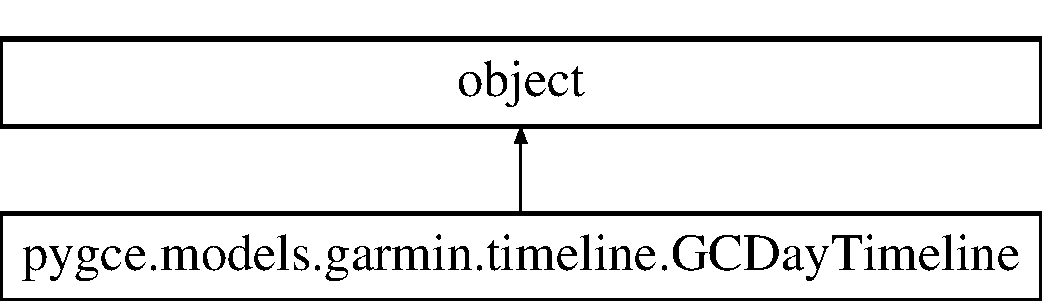
\includegraphics[height=2.000000cm]{classpygce_1_1models_1_1garmin_1_1timeline_1_1_g_c_day_timeline}
\end{center}
\end{figure}
\subsection*{Public Member Functions}
\begin{DoxyCompactItemize}
\item 
def \hyperlink{classpygce_1_1models_1_1garmin_1_1timeline_1_1_g_c_day_timeline_a7ac2fc2ad2c247d5ac64c393e9e3c31e}{\+\_\+\+\_\+init\+\_\+\+\_\+} (self, date\+\_\+time, summary\+\_\+html, steps\+\_\+section\+\_\+html, steps\+\_\+details\+\_\+html, sleep\+\_\+section\+\_\+html, activities\+\_\+section\+\_\+html, breakdown\+\_\+section\+\_\+html)
\item 
def \hyperlink{classpygce_1_1models_1_1garmin_1_1timeline_1_1_g_c_day_timeline_a868c632c33e0deb2b2ebfccfa35aa839}{parse} (self)
\item 
def \hyperlink{classpygce_1_1models_1_1garmin_1_1timeline_1_1_g_c_day_timeline_ae2d3f754907b22c3a87715fa8664cb5d}{\+\_\+\+\_\+getattr\+\_\+\+\_\+} (self, item)
\item 
def \hyperlink{classpygce_1_1models_1_1garmin_1_1timeline_1_1_g_c_day_timeline_aea84908a12fe244f70ef0c7d6f9875b7}{to\+\_\+dict} (self)
\item 
def \hyperlink{classpygce_1_1models_1_1garmin_1_1timeline_1_1_g_c_day_timeline_a89b4a28c05fc57f7588f9aea91c2f5f3}{to\+\_\+csv\+\_\+dict} (self)
\item 
def \hyperlink{classpygce_1_1models_1_1garmin_1_1timeline_1_1_g_c_day_timeline_a45e446687d33554cb53dea0a2d052c1a}{to\+\_\+json} (self)
\end{DoxyCompactItemize}
\subsection*{Public Attributes}
\begin{DoxyCompactItemize}
\item 
\hyperlink{classpygce_1_1models_1_1garmin_1_1timeline_1_1_g_c_day_timeline_a93fbc84cc4bfb4b01ec4678c512dc6f7}{date}
\item 
\hyperlink{classpygce_1_1models_1_1garmin_1_1timeline_1_1_g_c_day_timeline_a2e73f290ffe476624ddc495bb3edd19b}{sections}
\end{DoxyCompactItemize}


\subsection{Detailed Description}
\begin{DoxyVerb}Standard Garmin Connect timeline of day as in webpage.
Each standard day consists of different sections:
- summary (day, likes, comment, kcal)
- steps (total, goal, distance, avg daily)
- sleep (total, deep total, light total, awake total)
- activities (for each one: kcal, time, distance, type, name, link)
- breakdown (highly active %, active %, sedentary %, sleep %)
\end{DoxyVerb}
 

Definition at line 556 of file timeline.\+py.



\subsection{Constructor \& Destructor Documentation}
\mbox{\Hypertarget{classpygce_1_1models_1_1garmin_1_1timeline_1_1_g_c_day_timeline_a7ac2fc2ad2c247d5ac64c393e9e3c31e}\label{classpygce_1_1models_1_1garmin_1_1timeline_1_1_g_c_day_timeline_a7ac2fc2ad2c247d5ac64c393e9e3c31e}} 
\index{pygce\+::models\+::garmin\+::timeline\+::\+G\+C\+Day\+Timeline@{pygce\+::models\+::garmin\+::timeline\+::\+G\+C\+Day\+Timeline}!\+\_\+\+\_\+init\+\_\+\+\_\+@{\+\_\+\+\_\+init\+\_\+\+\_\+}}
\index{\+\_\+\+\_\+init\+\_\+\+\_\+@{\+\_\+\+\_\+init\+\_\+\+\_\+}!pygce\+::models\+::garmin\+::timeline\+::\+G\+C\+Day\+Timeline@{pygce\+::models\+::garmin\+::timeline\+::\+G\+C\+Day\+Timeline}}
\subsubsection{\texorpdfstring{\+\_\+\+\_\+init\+\_\+\+\_\+()}{\_\_init\_\_()}}
{\footnotesize\ttfamily def pygce.\+models.\+garmin.\+timeline.\+G\+C\+Day\+Timeline.\+\_\+\+\_\+init\+\_\+\+\_\+ (\begin{DoxyParamCaption}\item[{}]{self,  }\item[{}]{date\+\_\+time,  }\item[{}]{summary\+\_\+html,  }\item[{}]{steps\+\_\+section\+\_\+html,  }\item[{}]{steps\+\_\+details\+\_\+html,  }\item[{}]{sleep\+\_\+section\+\_\+html,  }\item[{}]{activities\+\_\+section\+\_\+html,  }\item[{}]{breakdown\+\_\+section\+\_\+html }\end{DoxyParamCaption})}

\begin{DoxyVerb}:param date_time: datetime
    Datetime of day
:param summary_html: str
    HTML source snippet with information about the day
:param steps_section_html: str
    HTML source snippet with information about daily steps
:param sleep_section_html: str
    HTML source snippet with information about daily sleep
:param activities_section_html: str
    HTML source snippet with information about daily activities
:param breakdown_section_html: str
    HTML source snippet with information about daily breakdown
\end{DoxyVerb}
 

Definition at line 570 of file timeline.\+py.



\subsection{Member Function Documentation}
\mbox{\Hypertarget{classpygce_1_1models_1_1garmin_1_1timeline_1_1_g_c_day_timeline_ae2d3f754907b22c3a87715fa8664cb5d}\label{classpygce_1_1models_1_1garmin_1_1timeline_1_1_g_c_day_timeline_ae2d3f754907b22c3a87715fa8664cb5d}} 
\index{pygce\+::models\+::garmin\+::timeline\+::\+G\+C\+Day\+Timeline@{pygce\+::models\+::garmin\+::timeline\+::\+G\+C\+Day\+Timeline}!\+\_\+\+\_\+getattr\+\_\+\+\_\+@{\+\_\+\+\_\+getattr\+\_\+\+\_\+}}
\index{\+\_\+\+\_\+getattr\+\_\+\+\_\+@{\+\_\+\+\_\+getattr\+\_\+\+\_\+}!pygce\+::models\+::garmin\+::timeline\+::\+G\+C\+Day\+Timeline@{pygce\+::models\+::garmin\+::timeline\+::\+G\+C\+Day\+Timeline}}
\subsubsection{\texorpdfstring{\+\_\+\+\_\+getattr\+\_\+\+\_\+()}{\_\_getattr\_\_()}}
{\footnotesize\ttfamily def pygce.\+models.\+garmin.\+timeline.\+G\+C\+Day\+Timeline.\+\_\+\+\_\+getattr\+\_\+\+\_\+ (\begin{DoxyParamCaption}\item[{}]{self,  }\item[{}]{item }\end{DoxyParamCaption})}



Definition at line 607 of file timeline.\+py.

\mbox{\Hypertarget{classpygce_1_1models_1_1garmin_1_1timeline_1_1_g_c_day_timeline_a868c632c33e0deb2b2ebfccfa35aa839}\label{classpygce_1_1models_1_1garmin_1_1timeline_1_1_g_c_day_timeline_a868c632c33e0deb2b2ebfccfa35aa839}} 
\index{pygce\+::models\+::garmin\+::timeline\+::\+G\+C\+Day\+Timeline@{pygce\+::models\+::garmin\+::timeline\+::\+G\+C\+Day\+Timeline}!parse@{parse}}
\index{parse@{parse}!pygce\+::models\+::garmin\+::timeline\+::\+G\+C\+Day\+Timeline@{pygce\+::models\+::garmin\+::timeline\+::\+G\+C\+Day\+Timeline}}
\subsubsection{\texorpdfstring{parse()}{parse()}}
{\footnotesize\ttfamily def pygce.\+models.\+garmin.\+timeline.\+G\+C\+Day\+Timeline.\+parse (\begin{DoxyParamCaption}\item[{}]{self }\end{DoxyParamCaption})}

\begin{DoxyVerb}:return: void
    Finds all sections to parse, then builds corresponding objects and parses everything
\end{DoxyVerb}
 

Definition at line 598 of file timeline.\+py.

\mbox{\Hypertarget{classpygce_1_1models_1_1garmin_1_1timeline_1_1_g_c_day_timeline_a89b4a28c05fc57f7588f9aea91c2f5f3}\label{classpygce_1_1models_1_1garmin_1_1timeline_1_1_g_c_day_timeline_a89b4a28c05fc57f7588f9aea91c2f5f3}} 
\index{pygce\+::models\+::garmin\+::timeline\+::\+G\+C\+Day\+Timeline@{pygce\+::models\+::garmin\+::timeline\+::\+G\+C\+Day\+Timeline}!to\+\_\+csv\+\_\+dict@{to\+\_\+csv\+\_\+dict}}
\index{to\+\_\+csv\+\_\+dict@{to\+\_\+csv\+\_\+dict}!pygce\+::models\+::garmin\+::timeline\+::\+G\+C\+Day\+Timeline@{pygce\+::models\+::garmin\+::timeline\+::\+G\+C\+Day\+Timeline}}
\subsubsection{\texorpdfstring{to\+\_\+csv\+\_\+dict()}{to\_csv\_dict()}}
{\footnotesize\ttfamily def pygce.\+models.\+garmin.\+timeline.\+G\+C\+Day\+Timeline.\+to\+\_\+csv\+\_\+dict (\begin{DoxyParamCaption}\item[{}]{self }\end{DoxyParamCaption})}

\begin{DoxyVerb}:return: {}
    Like self.to_dict() but with a set with keys and values NOT nested. Also for activities there are totals only
\end{DoxyVerb}
 

Definition at line 618 of file timeline.\+py.

\mbox{\Hypertarget{classpygce_1_1models_1_1garmin_1_1timeline_1_1_g_c_day_timeline_aea84908a12fe244f70ef0c7d6f9875b7}\label{classpygce_1_1models_1_1garmin_1_1timeline_1_1_g_c_day_timeline_aea84908a12fe244f70ef0c7d6f9875b7}} 
\index{pygce\+::models\+::garmin\+::timeline\+::\+G\+C\+Day\+Timeline@{pygce\+::models\+::garmin\+::timeline\+::\+G\+C\+Day\+Timeline}!to\+\_\+dict@{to\+\_\+dict}}
\index{to\+\_\+dict@{to\+\_\+dict}!pygce\+::models\+::garmin\+::timeline\+::\+G\+C\+Day\+Timeline@{pygce\+::models\+::garmin\+::timeline\+::\+G\+C\+Day\+Timeline}}
\subsubsection{\texorpdfstring{to\+\_\+dict()}{to\_dict()}}
{\footnotesize\ttfamily def pygce.\+models.\+garmin.\+timeline.\+G\+C\+Day\+Timeline.\+to\+\_\+dict (\begin{DoxyParamCaption}\item[{}]{self }\end{DoxyParamCaption})}

\begin{DoxyVerb}:return: dict
    Dictionary with keys (obj fields) and values (obj values)
\end{DoxyVerb}
 

Definition at line 610 of file timeline.\+py.

\mbox{\Hypertarget{classpygce_1_1models_1_1garmin_1_1timeline_1_1_g_c_day_timeline_a45e446687d33554cb53dea0a2d052c1a}\label{classpygce_1_1models_1_1garmin_1_1timeline_1_1_g_c_day_timeline_a45e446687d33554cb53dea0a2d052c1a}} 
\index{pygce\+::models\+::garmin\+::timeline\+::\+G\+C\+Day\+Timeline@{pygce\+::models\+::garmin\+::timeline\+::\+G\+C\+Day\+Timeline}!to\+\_\+json@{to\+\_\+json}}
\index{to\+\_\+json@{to\+\_\+json}!pygce\+::models\+::garmin\+::timeline\+::\+G\+C\+Day\+Timeline@{pygce\+::models\+::garmin\+::timeline\+::\+G\+C\+Day\+Timeline}}
\subsubsection{\texorpdfstring{to\+\_\+json()}{to\_json()}}
{\footnotesize\ttfamily def pygce.\+models.\+garmin.\+timeline.\+G\+C\+Day\+Timeline.\+to\+\_\+json (\begin{DoxyParamCaption}\item[{}]{self }\end{DoxyParamCaption})}

\begin{DoxyVerb}:return: json object
    A json representation of this object
\end{DoxyVerb}
 

Definition at line 632 of file timeline.\+py.



\subsection{Member Data Documentation}
\mbox{\Hypertarget{classpygce_1_1models_1_1garmin_1_1timeline_1_1_g_c_day_timeline_a93fbc84cc4bfb4b01ec4678c512dc6f7}\label{classpygce_1_1models_1_1garmin_1_1timeline_1_1_g_c_day_timeline_a93fbc84cc4bfb4b01ec4678c512dc6f7}} 
\index{pygce\+::models\+::garmin\+::timeline\+::\+G\+C\+Day\+Timeline@{pygce\+::models\+::garmin\+::timeline\+::\+G\+C\+Day\+Timeline}!date@{date}}
\index{date@{date}!pygce\+::models\+::garmin\+::timeline\+::\+G\+C\+Day\+Timeline@{pygce\+::models\+::garmin\+::timeline\+::\+G\+C\+Day\+Timeline}}
\subsubsection{\texorpdfstring{date}{date}}
{\footnotesize\ttfamily pygce.\+models.\+garmin.\+timeline.\+G\+C\+Day\+Timeline.\+date}



Definition at line 588 of file timeline.\+py.

\mbox{\Hypertarget{classpygce_1_1models_1_1garmin_1_1timeline_1_1_g_c_day_timeline_a2e73f290ffe476624ddc495bb3edd19b}\label{classpygce_1_1models_1_1garmin_1_1timeline_1_1_g_c_day_timeline_a2e73f290ffe476624ddc495bb3edd19b}} 
\index{pygce\+::models\+::garmin\+::timeline\+::\+G\+C\+Day\+Timeline@{pygce\+::models\+::garmin\+::timeline\+::\+G\+C\+Day\+Timeline}!sections@{sections}}
\index{sections@{sections}!pygce\+::models\+::garmin\+::timeline\+::\+G\+C\+Day\+Timeline@{pygce\+::models\+::garmin\+::timeline\+::\+G\+C\+Day\+Timeline}}
\subsubsection{\texorpdfstring{sections}{sections}}
{\footnotesize\ttfamily pygce.\+models.\+garmin.\+timeline.\+G\+C\+Day\+Timeline.\+sections}



Definition at line 589 of file timeline.\+py.



The documentation for this class was generated from the following file\+:\begin{DoxyCompactItemize}
\item 
/home/stefano/\+Coding/\+Python/\+\_\+projects/pygce/pygce/models/garmin/\hyperlink{timeline_8py}{timeline.\+py}\end{DoxyCompactItemize}

\hypertarget{classpygce_1_1analysis_1_1models_1_1_m_l_analysis}{}\section{pygce.\+analysis.\+models.\+M\+L\+Analysis Class Reference}
\label{classpygce_1_1analysis_1_1models_1_1_m_l_analysis}\index{pygce.\+analysis.\+models.\+M\+L\+Analysis@{pygce.\+analysis.\+models.\+M\+L\+Analysis}}
Inheritance diagram for pygce.\+analysis.\+models.\+M\+L\+Analysis\+:\begin{figure}[H]
\begin{center}
\leavevmode
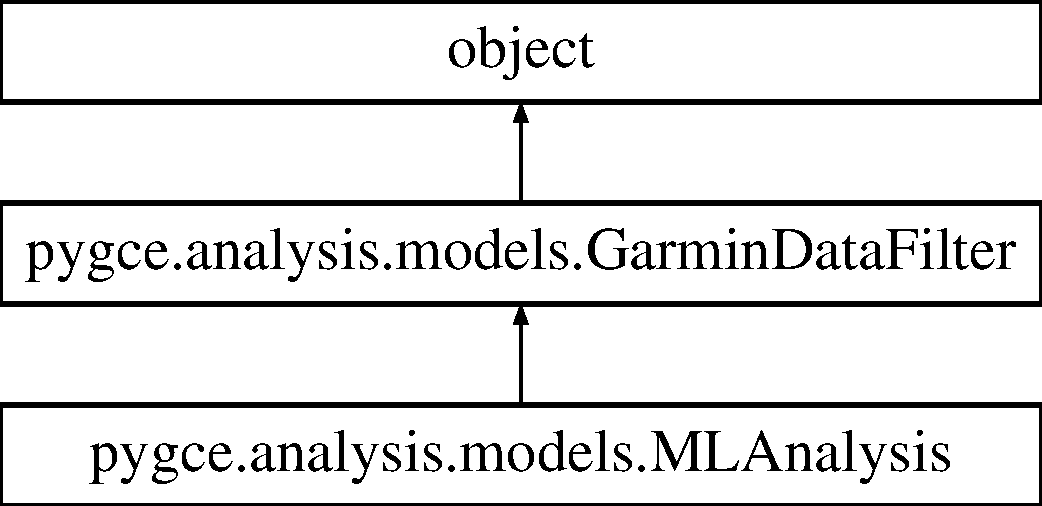
\includegraphics[height=3.000000cm]{classpygce_1_1analysis_1_1models_1_1_m_l_analysis}
\end{center}
\end{figure}
\subsection*{Public Member Functions}
\begin{DoxyCompactItemize}
\item 
def \hyperlink{classpygce_1_1analysis_1_1models_1_1_m_l_analysis_a87a6dea18d5aa1163763e66f0142dca8}{\+\_\+\+\_\+init\+\_\+\+\_\+} (self, \hyperlink{classpygce_1_1analysis_1_1models_1_1_garmin_data_filter_a7bb7be05577c2d31546e27823a5d11c5}{dataset\+\_\+file})
\end{DoxyCompactItemize}
\subsection*{Additional Inherited Members}


\subsection{Detailed Description}
\begin{DoxyVerb}Carries out popular machine-learning tasks on Garmin data \end{DoxyVerb}
 

Definition at line 125 of file models.\+py.



\subsection{Constructor \& Destructor Documentation}
\index{pygce\+::analysis\+::models\+::\+M\+L\+Analysis@{pygce\+::analysis\+::models\+::\+M\+L\+Analysis}!\+\_\+\+\_\+init\+\_\+\+\_\+@{\+\_\+\+\_\+init\+\_\+\+\_\+}}
\index{\+\_\+\+\_\+init\+\_\+\+\_\+@{\+\_\+\+\_\+init\+\_\+\+\_\+}!pygce\+::analysis\+::models\+::\+M\+L\+Analysis@{pygce\+::analysis\+::models\+::\+M\+L\+Analysis}}
\subsubsection[{\texorpdfstring{\+\_\+\+\_\+init\+\_\+\+\_\+(self, dataset\+\_\+file)}{__init__(self, dataset_file)}}]{\setlength{\rightskip}{0pt plus 5cm}def pygce.\+analysis.\+models.\+M\+L\+Analysis.\+\_\+\+\_\+init\+\_\+\+\_\+ (
\begin{DoxyParamCaption}
\item[{}]{self, }
\item[{}]{dataset\+\_\+file}
\end{DoxyParamCaption}
)}\hypertarget{classpygce_1_1analysis_1_1models_1_1_m_l_analysis_a87a6dea18d5aa1163763e66f0142dca8}{}\label{classpygce_1_1analysis_1_1models_1_1_m_l_analysis_a87a6dea18d5aa1163763e66f0142dca8}
\begin{DoxyVerb}:param dataset_file: str
    Path to folder with data to analyse
\end{DoxyVerb}
 

Definition at line 128 of file models.\+py.



The documentation for this class was generated from the following file\+:\begin{DoxyCompactItemize}
\item 
/home/stefano/\+Coding/\+Python/projects/garmin-\/connect-\/export/pygce/analysis/\hyperlink{models_8py}{models.\+py}\end{DoxyCompactItemize}

\hypertarget{classpygce_1_1analysis_1_1models_1_1_stats_analysis}{}\section{pygce.\+analysis.\+models.\+Stats\+Analysis Class Reference}
\label{classpygce_1_1analysis_1_1models_1_1_stats_analysis}\index{pygce.\+analysis.\+models.\+Stats\+Analysis@{pygce.\+analysis.\+models.\+Stats\+Analysis}}
Inheritance diagram for pygce.\+analysis.\+models.\+Stats\+Analysis\+:\begin{figure}[H]
\begin{center}
\leavevmode
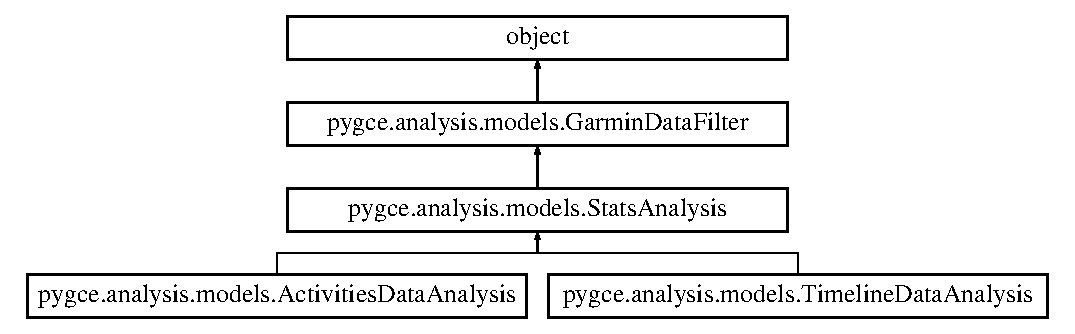
\includegraphics[height=4.000000cm]{classpygce_1_1analysis_1_1models_1_1_stats_analysis}
\end{center}
\end{figure}
\subsection*{Public Member Functions}
\begin{DoxyCompactItemize}
\item 
def \hyperlink{classpygce_1_1analysis_1_1models_1_1_stats_analysis_a161706ff9c5a5410356e28a240ea5e29}{\+\_\+\+\_\+init\+\_\+\+\_\+} (self, \hyperlink{classpygce_1_1analysis_1_1models_1_1_garmin_data_filter_a7bb7be05577c2d31546e27823a5d11c5}{dataset\+\_\+file})
\item 
def \hyperlink{classpygce_1_1analysis_1_1models_1_1_stats_analysis_a2dd9052d1133c137c3049c6a425f8722}{show\+\_\+correlation\+\_\+matrix} (self, title\+\_\+image, headers\+\_\+to\+\_\+analyze)
\end{DoxyCompactItemize}
\subsection*{Additional Inherited Members}


\subsection{Detailed Description}
\begin{DoxyVerb}Computes correlation of data\end{DoxyVerb}
 

Definition at line 91 of file models.\+py.



\subsection{Constructor \& Destructor Documentation}
\index{pygce\+::analysis\+::models\+::\+Stats\+Analysis@{pygce\+::analysis\+::models\+::\+Stats\+Analysis}!\+\_\+\+\_\+init\+\_\+\+\_\+@{\+\_\+\+\_\+init\+\_\+\+\_\+}}
\index{\+\_\+\+\_\+init\+\_\+\+\_\+@{\+\_\+\+\_\+init\+\_\+\+\_\+}!pygce\+::analysis\+::models\+::\+Stats\+Analysis@{pygce\+::analysis\+::models\+::\+Stats\+Analysis}}
\subsubsection[{\texorpdfstring{\+\_\+\+\_\+init\+\_\+\+\_\+(self, dataset\+\_\+file)}{__init__(self, dataset_file)}}]{\setlength{\rightskip}{0pt plus 5cm}def pygce.\+analysis.\+models.\+Stats\+Analysis.\+\_\+\+\_\+init\+\_\+\+\_\+ (
\begin{DoxyParamCaption}
\item[{}]{self, }
\item[{}]{dataset\+\_\+file}
\end{DoxyParamCaption}
)}\hypertarget{classpygce_1_1analysis_1_1models_1_1_stats_analysis_a161706ff9c5a5410356e28a240ea5e29}{}\label{classpygce_1_1analysis_1_1models_1_1_stats_analysis_a161706ff9c5a5410356e28a240ea5e29}
\begin{DoxyVerb}:param dataset_file: str
    Path to folder with data to analyse
\end{DoxyVerb}
 

Definition at line 94 of file models.\+py.



\subsection{Member Function Documentation}
\index{pygce\+::analysis\+::models\+::\+Stats\+Analysis@{pygce\+::analysis\+::models\+::\+Stats\+Analysis}!show\+\_\+correlation\+\_\+matrix@{show\+\_\+correlation\+\_\+matrix}}
\index{show\+\_\+correlation\+\_\+matrix@{show\+\_\+correlation\+\_\+matrix}!pygce\+::analysis\+::models\+::\+Stats\+Analysis@{pygce\+::analysis\+::models\+::\+Stats\+Analysis}}
\subsubsection[{\texorpdfstring{show\+\_\+correlation\+\_\+matrix(self, title\+\_\+image, headers\+\_\+to\+\_\+analyze)}{show_correlation_matrix(self, title_image, headers_to_analyze)}}]{\setlength{\rightskip}{0pt plus 5cm}def pygce.\+analysis.\+models.\+Stats\+Analysis.\+show\+\_\+correlation\+\_\+matrix (
\begin{DoxyParamCaption}
\item[{}]{self, }
\item[{}]{title\+\_\+image, }
\item[{}]{headers\+\_\+to\+\_\+analyze}
\end{DoxyParamCaption}
)}\hypertarget{classpygce_1_1analysis_1_1models_1_1_stats_analysis_a2dd9052d1133c137c3049c6a425f8722}{}\label{classpygce_1_1analysis_1_1models_1_1_stats_analysis_a2dd9052d1133c137c3049c6a425f8722}
\begin{DoxyVerb}:param title_image: str
    Title of output image
:param headers_to_analyze: [] of str
    Compute correlation matrix of only these headers
:return: void
    Shows correlation matrix of data of files in folder
\end{DoxyVerb}
 

Definition at line 102 of file models.\+py.



The documentation for this class was generated from the following file\+:\begin{DoxyCompactItemize}
\item 
/home/stefano/\+Coding/\+Python/projects/garmin-\/connect-\/export/pygce/analysis/\hyperlink{models_8py}{models.\+py}\end{DoxyCompactItemize}

\hypertarget{classpygce_1_1analysis_1_1models_1_1_timeline_data_analysis}{}\section{pygce.\+analysis.\+models.\+Timeline\+Data\+Analysis Class Reference}
\label{classpygce_1_1analysis_1_1models_1_1_timeline_data_analysis}\index{pygce.\+analysis.\+models.\+Timeline\+Data\+Analysis@{pygce.\+analysis.\+models.\+Timeline\+Data\+Analysis}}
Inheritance diagram for pygce.\+analysis.\+models.\+Timeline\+Data\+Analysis\+:\begin{figure}[H]
\begin{center}
\leavevmode
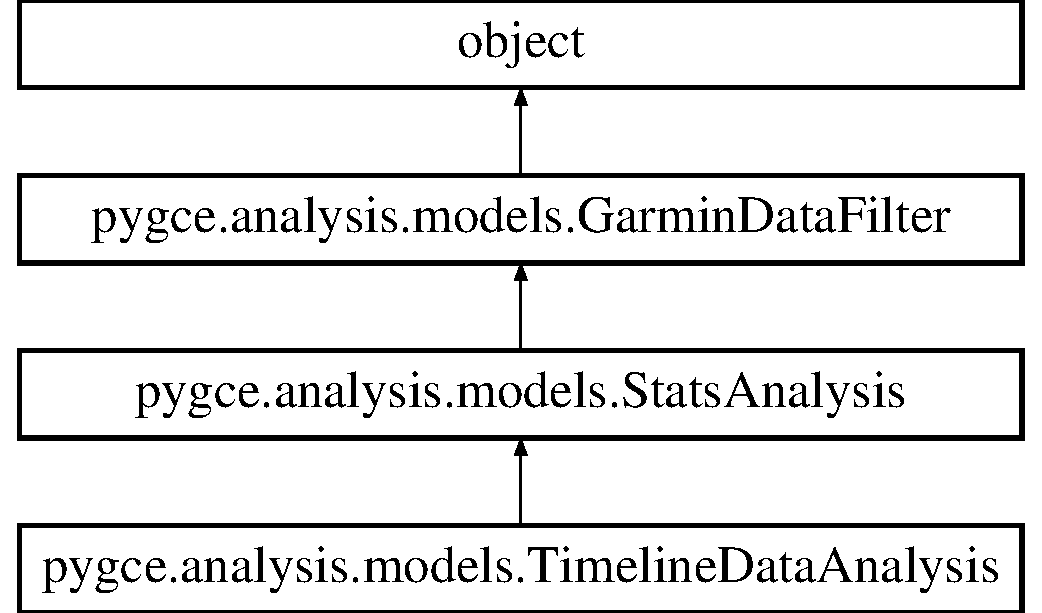
\includegraphics[height=4.000000cm]{classpygce_1_1analysis_1_1models_1_1_timeline_data_analysis}
\end{center}
\end{figure}
\subsection*{Public Member Functions}
\begin{DoxyCompactItemize}
\item 
def \hyperlink{classpygce_1_1analysis_1_1models_1_1_timeline_data_analysis_a7fccb7531cafe3b618ad7026db2d3b53}{\+\_\+\+\_\+init\+\_\+\+\_\+} (self, \hyperlink{classpygce_1_1analysis_1_1models_1_1_garmin_data_filter_a7bb7be05577c2d31546e27823a5d11c5}{dataset\+\_\+file})
\item 
def \hyperlink{classpygce_1_1analysis_1_1models_1_1_timeline_data_analysis_a1a02ca1184152091fc1f66306e1ac02c}{parse\+\_\+csv} (self)
\item 
def \hyperlink{classpygce_1_1analysis_1_1models_1_1_timeline_data_analysis_ac5f4540c89ea52ccbd5c28ce850bc1d3}{show\+\_\+correlation\+\_\+matrix\+\_\+of\+\_\+data} (self)
\item 
def \hyperlink{classpygce_1_1analysis_1_1models_1_1_timeline_data_analysis_ab769c6f075333081a68712e0ecf8b094}{predict\+\_\+feature} (self, feature)
\item 
def \hyperlink{classpygce_1_1analysis_1_1models_1_1_timeline_data_analysis_a4bdbc9b67a365b2e0d5a76e7bd811ce5}{cluster\+\_\+analyze} (self, n\+\_\+clusters=6)
\end{DoxyCompactItemize}
\subsection*{Static Public Attributes}
\begin{DoxyCompactItemize}
\item 
list \hyperlink{classpygce_1_1analysis_1_1models_1_1_timeline_data_analysis_abc835b2b9b9d8555a2b49e8534782021}{H\+E\+A\+D\+E\+R\+S\+\_\+\+T\+O\+\_\+\+A\+N\+A\+L\+Y\+ZE}
\item 
list \hyperlink{classpygce_1_1analysis_1_1models_1_1_timeline_data_analysis_afaebf4ce7e847ff4c32a7b9b799fd94d}{T\+I\+M\+E\+\_\+\+H\+E\+A\+D\+E\+R\+S\+\_\+\+T\+O\+\_\+\+C\+O\+N\+V\+E\+RT}
\end{DoxyCompactItemize}
\subsection*{Additional Inherited Members}


\subsection{Detailed Description}
\begin{DoxyVerb}Machine-learn timeline data \end{DoxyVerb}
 

Definition at line 123 of file models.\+py.



\subsection{Constructor \& Destructor Documentation}
\index{pygce\+::analysis\+::models\+::\+Timeline\+Data\+Analysis@{pygce\+::analysis\+::models\+::\+Timeline\+Data\+Analysis}!\+\_\+\+\_\+init\+\_\+\+\_\+@{\+\_\+\+\_\+init\+\_\+\+\_\+}}
\index{\+\_\+\+\_\+init\+\_\+\+\_\+@{\+\_\+\+\_\+init\+\_\+\+\_\+}!pygce\+::analysis\+::models\+::\+Timeline\+Data\+Analysis@{pygce\+::analysis\+::models\+::\+Timeline\+Data\+Analysis}}
\subsubsection[{\texorpdfstring{\+\_\+\+\_\+init\+\_\+\+\_\+(self, dataset\+\_\+file)}{__init__(self, dataset_file)}}]{\setlength{\rightskip}{0pt plus 5cm}def pygce.\+analysis.\+models.\+Timeline\+Data\+Analysis.\+\_\+\+\_\+init\+\_\+\+\_\+ (
\begin{DoxyParamCaption}
\item[{}]{self, }
\item[{}]{dataset\+\_\+file}
\end{DoxyParamCaption}
)}\hypertarget{classpygce_1_1analysis_1_1models_1_1_timeline_data_analysis_a7fccb7531cafe3b618ad7026db2d3b53}{}\label{classpygce_1_1analysis_1_1models_1_1_timeline_data_analysis_a7fccb7531cafe3b618ad7026db2d3b53}
\begin{DoxyVerb}:param dataset_file: str
    Path to folder with data to analyse
\end{DoxyVerb}
 

Definition at line 155 of file models.\+py.



\subsection{Member Function Documentation}
\index{pygce\+::analysis\+::models\+::\+Timeline\+Data\+Analysis@{pygce\+::analysis\+::models\+::\+Timeline\+Data\+Analysis}!cluster\+\_\+analyze@{cluster\+\_\+analyze}}
\index{cluster\+\_\+analyze@{cluster\+\_\+analyze}!pygce\+::analysis\+::models\+::\+Timeline\+Data\+Analysis@{pygce\+::analysis\+::models\+::\+Timeline\+Data\+Analysis}}
\subsubsection[{\texorpdfstring{cluster\+\_\+analyze(self, n\+\_\+clusters=6)}{cluster_analyze(self, n_clusters=6)}}]{\setlength{\rightskip}{0pt plus 5cm}def pygce.\+analysis.\+models.\+Timeline\+Data\+Analysis.\+cluster\+\_\+analyze (
\begin{DoxyParamCaption}
\item[{}]{self, }
\item[{}]{n\+\_\+clusters = {\ttfamily 6}}
\end{DoxyParamCaption}
)}\hypertarget{classpygce_1_1analysis_1_1models_1_1_timeline_data_analysis_a4bdbc9b67a365b2e0d5a76e7bd811ce5}{}\label{classpygce_1_1analysis_1_1models_1_1_timeline_data_analysis_a4bdbc9b67a365b2e0d5a76e7bd811ce5}
\begin{DoxyVerb}:param n_clusters: int
    Number of clusters
:return: void
    Computes cluster analysis: see days based on differences.
    Each day is different from one another, there are days where you trained more, others where you ate more ...
    The goal is to divide your days into categories (e.g highly-active, active ...) based on data logs.
    This way, the input matrix consists of multiple vectors with each one consisting of one day's values.
\end{DoxyVerb}
 

Definition at line 208 of file models.\+py.

\index{pygce\+::analysis\+::models\+::\+Timeline\+Data\+Analysis@{pygce\+::analysis\+::models\+::\+Timeline\+Data\+Analysis}!parse\+\_\+csv@{parse\+\_\+csv}}
\index{parse\+\_\+csv@{parse\+\_\+csv}!pygce\+::analysis\+::models\+::\+Timeline\+Data\+Analysis@{pygce\+::analysis\+::models\+::\+Timeline\+Data\+Analysis}}
\subsubsection[{\texorpdfstring{parse\+\_\+csv(self)}{parse_csv(self)}}]{\setlength{\rightskip}{0pt plus 5cm}def pygce.\+analysis.\+models.\+Timeline\+Data\+Analysis.\+parse\+\_\+csv (
\begin{DoxyParamCaption}
\item[{}]{self}
\end{DoxyParamCaption}
)}\hypertarget{classpygce_1_1analysis_1_1models_1_1_timeline_data_analysis_a1a02ca1184152091fc1f66306e1ac02c}{}\label{classpygce_1_1analysis_1_1models_1_1_timeline_data_analysis_a1a02ca1184152091fc1f66306e1ac02c}
\begin{DoxyVerb}:return: tuple [], [] of []
    Headers of csv file and data
\end{DoxyVerb}
 

Definition at line 163 of file models.\+py.

\index{pygce\+::analysis\+::models\+::\+Timeline\+Data\+Analysis@{pygce\+::analysis\+::models\+::\+Timeline\+Data\+Analysis}!predict\+\_\+feature@{predict\+\_\+feature}}
\index{predict\+\_\+feature@{predict\+\_\+feature}!pygce\+::analysis\+::models\+::\+Timeline\+Data\+Analysis@{pygce\+::analysis\+::models\+::\+Timeline\+Data\+Analysis}}
\subsubsection[{\texorpdfstring{predict\+\_\+feature(self, feature)}{predict_feature(self, feature)}}]{\setlength{\rightskip}{0pt plus 5cm}def pygce.\+analysis.\+models.\+Timeline\+Data\+Analysis.\+predict\+\_\+feature (
\begin{DoxyParamCaption}
\item[{}]{self, }
\item[{}]{feature}
\end{DoxyParamCaption}
)}\hypertarget{classpygce_1_1analysis_1_1models_1_1_timeline_data_analysis_ab769c6f075333081a68712e0ecf8b094}{}\label{classpygce_1_1analysis_1_1models_1_1_timeline_data_analysis_ab769c6f075333081a68712e0ecf8b094}
\begin{DoxyVerb}:param feature: str
    Name of feature (column name) to predict
:return: TODO
    TODO
\end{DoxyVerb}
 

Definition at line 182 of file models.\+py.

\index{pygce\+::analysis\+::models\+::\+Timeline\+Data\+Analysis@{pygce\+::analysis\+::models\+::\+Timeline\+Data\+Analysis}!show\+\_\+correlation\+\_\+matrix\+\_\+of\+\_\+data@{show\+\_\+correlation\+\_\+matrix\+\_\+of\+\_\+data}}
\index{show\+\_\+correlation\+\_\+matrix\+\_\+of\+\_\+data@{show\+\_\+correlation\+\_\+matrix\+\_\+of\+\_\+data}!pygce\+::analysis\+::models\+::\+Timeline\+Data\+Analysis@{pygce\+::analysis\+::models\+::\+Timeline\+Data\+Analysis}}
\subsubsection[{\texorpdfstring{show\+\_\+correlation\+\_\+matrix\+\_\+of\+\_\+data(self)}{show_correlation_matrix_of_data(self)}}]{\setlength{\rightskip}{0pt plus 5cm}def pygce.\+analysis.\+models.\+Timeline\+Data\+Analysis.\+show\+\_\+correlation\+\_\+matrix\+\_\+of\+\_\+data (
\begin{DoxyParamCaption}
\item[{}]{self}
\end{DoxyParamCaption}
)}\hypertarget{classpygce_1_1analysis_1_1models_1_1_timeline_data_analysis_ac5f4540c89ea52ccbd5c28ce850bc1d3}{}\label{classpygce_1_1analysis_1_1models_1_1_timeline_data_analysis_ac5f4540c89ea52ccbd5c28ce850bc1d3}
\begin{DoxyVerb}:return: void
    Shows correlation matrix of data of files in folder
\end{DoxyVerb}
 

Definition at line 173 of file models.\+py.



\subsection{Member Data Documentation}
\index{pygce\+::analysis\+::models\+::\+Timeline\+Data\+Analysis@{pygce\+::analysis\+::models\+::\+Timeline\+Data\+Analysis}!H\+E\+A\+D\+E\+R\+S\+\_\+\+T\+O\+\_\+\+A\+N\+A\+L\+Y\+ZE@{H\+E\+A\+D\+E\+R\+S\+\_\+\+T\+O\+\_\+\+A\+N\+A\+L\+Y\+ZE}}
\index{H\+E\+A\+D\+E\+R\+S\+\_\+\+T\+O\+\_\+\+A\+N\+A\+L\+Y\+ZE@{H\+E\+A\+D\+E\+R\+S\+\_\+\+T\+O\+\_\+\+A\+N\+A\+L\+Y\+ZE}!pygce\+::analysis\+::models\+::\+Timeline\+Data\+Analysis@{pygce\+::analysis\+::models\+::\+Timeline\+Data\+Analysis}}
\subsubsection[{\texorpdfstring{H\+E\+A\+D\+E\+R\+S\+\_\+\+T\+O\+\_\+\+A\+N\+A\+L\+Y\+ZE}{HEADERS_TO_ANALYZE}}]{\setlength{\rightskip}{0pt plus 5cm}list pygce.\+analysis.\+models.\+Timeline\+Data\+Analysis.\+H\+E\+A\+D\+E\+R\+S\+\_\+\+T\+O\+\_\+\+A\+N\+A\+L\+Y\+ZE\hspace{0.3cm}{\ttfamily [static]}}\hypertarget{classpygce_1_1analysis_1_1models_1_1_timeline_data_analysis_abc835b2b9b9d8555a2b49e8534782021}{}\label{classpygce_1_1analysis_1_1models_1_1_timeline_data_analysis_abc835b2b9b9d8555a2b49e8534782021}
{\bfseries Initial value\+:}
\begin{DoxyCode}
1 = [
2         \textcolor{stringliteral}{"SUMMARY:kcal\_count"},
3         \textcolor{stringliteral}{"STEPS:distance"},
4         \textcolor{stringliteral}{"SLEEP:light\_sleep\_time"},
5         \textcolor{stringliteral}{"BREAKDOWN:sleeping"},
6         \textcolor{stringliteral}{"BREAKDOWN:highly\_active"},
7         \textcolor{stringliteral}{"ACTIVITIES:kcal"},
8         \textcolor{stringliteral}{"BREAKDOWN:active"},
9         \textcolor{stringliteral}{"STEPS:total"},
10         \textcolor{stringliteral}{"STEPS:avg"},
11         \textcolor{stringliteral}{"BREAKDOWN:sedentary"},
12         \textcolor{stringliteral}{"SLEEP:awake\_sleep\_time"},
13         \textcolor{stringliteral}{"SLEEP:total\_sleep\_time"},
14         \textcolor{stringliteral}{"SLEEP:deep\_sleep\_time"},
15         \textcolor{stringliteral}{"ACTIVITIES:duration"},
16         \textcolor{stringliteral}{"ACTIVITIES:distance"},
17         \textcolor{stringliteral}{"STEPS:goal"},
18         \textcolor{stringliteral}{"SLEEP:night\_sleep\_time"}
19     ]
\end{DoxyCode}


Definition at line 126 of file models.\+py.

\index{pygce\+::analysis\+::models\+::\+Timeline\+Data\+Analysis@{pygce\+::analysis\+::models\+::\+Timeline\+Data\+Analysis}!T\+I\+M\+E\+\_\+\+H\+E\+A\+D\+E\+R\+S\+\_\+\+T\+O\+\_\+\+C\+O\+N\+V\+E\+RT@{T\+I\+M\+E\+\_\+\+H\+E\+A\+D\+E\+R\+S\+\_\+\+T\+O\+\_\+\+C\+O\+N\+V\+E\+RT}}
\index{T\+I\+M\+E\+\_\+\+H\+E\+A\+D\+E\+R\+S\+\_\+\+T\+O\+\_\+\+C\+O\+N\+V\+E\+RT@{T\+I\+M\+E\+\_\+\+H\+E\+A\+D\+E\+R\+S\+\_\+\+T\+O\+\_\+\+C\+O\+N\+V\+E\+RT}!pygce\+::analysis\+::models\+::\+Timeline\+Data\+Analysis@{pygce\+::analysis\+::models\+::\+Timeline\+Data\+Analysis}}
\subsubsection[{\texorpdfstring{T\+I\+M\+E\+\_\+\+H\+E\+A\+D\+E\+R\+S\+\_\+\+T\+O\+\_\+\+C\+O\+N\+V\+E\+RT}{TIME_HEADERS_TO_CONVERT}}]{\setlength{\rightskip}{0pt plus 5cm}list pygce.\+analysis.\+models.\+Timeline\+Data\+Analysis.\+T\+I\+M\+E\+\_\+\+H\+E\+A\+D\+E\+R\+S\+\_\+\+T\+O\+\_\+\+C\+O\+N\+V\+E\+RT\hspace{0.3cm}{\ttfamily [static]}}\hypertarget{classpygce_1_1analysis_1_1models_1_1_timeline_data_analysis_afaebf4ce7e847ff4c32a7b9b799fd94d}{}\label{classpygce_1_1analysis_1_1models_1_1_timeline_data_analysis_afaebf4ce7e847ff4c32a7b9b799fd94d}
{\bfseries Initial value\+:}
\begin{DoxyCode}
1 = [
2         \textcolor{stringliteral}{"SLEEP:nap\_time"},
3         \textcolor{stringliteral}{"SLEEP:light\_sleep\_time"},
4         \textcolor{stringliteral}{"SLEEP:awake\_sleep\_time"},
5         \textcolor{stringliteral}{"SLEEP:total\_sleep\_time"},
6         \textcolor{stringliteral}{"SLEEP:deep\_sleep\_time"},
7         \textcolor{stringliteral}{"SLEEP:night\_sleep\_time"},
8         \textcolor{stringliteral}{"ACTIVITIES:duration"}
9     ]
\end{DoxyCode}


Definition at line 145 of file models.\+py.



The documentation for this class was generated from the following file\+:\begin{DoxyCompactItemize}
\item 
/home/stefano/\+Coding/\+Python/projects/garmin-\/connect-\/export/pygce/analysis/\hyperlink{models_8py}{models.\+py}\end{DoxyCompactItemize}

\chapter{File Documentation}
\hypertarget{____init_____8py}{}\section{/home/stefano/\+Coding/\+Python/projects/garmin-\/connect-\/export/pygce/\+\_\+\+\_\+init\+\_\+\+\_\+.py File Reference}
\label{____init_____8py}\index{/home/stefano/\+Coding/\+Python/projects/garmin-\/connect-\/export/pygce/\+\_\+\+\_\+init\+\_\+\+\_\+.\+py@{/home/stefano/\+Coding/\+Python/projects/garmin-\/connect-\/export/pygce/\+\_\+\+\_\+init\+\_\+\+\_\+.\+py}}
\subsection*{Namespaces}
\begin{DoxyCompactItemize}
\item 
 \hyperlink{namespacepygce}{pygce}
\end{DoxyCompactItemize}

\hypertarget{analysis_2____init_____8py}{}\section{/home/stefano/\+Coding/\+Python/projects/pygce/pygce/analysis/\+\_\+\+\_\+init\+\_\+\+\_\+.py File Reference}
\label{analysis_2____init_____8py}\index{/home/stefano/\+Coding/\+Python/projects/pygce/pygce/analysis/\+\_\+\+\_\+init\+\_\+\+\_\+.\+py@{/home/stefano/\+Coding/\+Python/projects/pygce/pygce/analysis/\+\_\+\+\_\+init\+\_\+\+\_\+.\+py}}
\subsection*{Namespaces}
\begin{DoxyCompactItemize}
\item 
 \hyperlink{namespacepygce_1_1analysis}{pygce.\+analysis}
\end{DoxyCompactItemize}

\hypertarget{models_2____init_____8py}{}\section{/home/stefano/\+Coding/\+Python/projects/garmin-\/connect-\/export/pygce/models/\+\_\+\+\_\+init\+\_\+\+\_\+.py File Reference}
\label{models_2____init_____8py}\index{/home/stefano/\+Coding/\+Python/projects/garmin-\/connect-\/export/pygce/models/\+\_\+\+\_\+init\+\_\+\+\_\+.\+py@{/home/stefano/\+Coding/\+Python/projects/garmin-\/connect-\/export/pygce/models/\+\_\+\+\_\+init\+\_\+\+\_\+.\+py}}
\subsection*{Namespaces}
\begin{DoxyCompactItemize}
\item 
 \hyperlink{namespacepygce_1_1models}{pygce.\+models}
\end{DoxyCompactItemize}

\hypertarget{models_2garmin_2____init_____8py}{}\section{/home/stefano/\+Coding/\+Python/\+\_\+projects/pygce/pygce/models/garmin/\+\_\+\+\_\+init\+\_\+\+\_\+.py File Reference}
\label{models_2garmin_2____init_____8py}\index{/home/stefano/\+Coding/\+Python/\+\_\+projects/pygce/pygce/models/garmin/\+\_\+\+\_\+init\+\_\+\+\_\+.\+py@{/home/stefano/\+Coding/\+Python/\+\_\+projects/pygce/pygce/models/garmin/\+\_\+\+\_\+init\+\_\+\+\_\+.\+py}}
\subsection*{Namespaces}
\begin{DoxyCompactItemize}
\item 
 \hyperlink{namespacepygce_1_1models_1_1garmin}{pygce.\+models.\+garmin}
\end{DoxyCompactItemize}

\hypertarget{analysis_2cli_8py}{}\section{/home/stefano/\+Coding/\+Python/projects/garmin-\/connect-\/export/pygce/analysis/cli.py File Reference}
\label{analysis_2cli_8py}\index{/home/stefano/\+Coding/\+Python/projects/garmin-\/connect-\/export/pygce/analysis/cli.\+py@{/home/stefano/\+Coding/\+Python/projects/garmin-\/connect-\/export/pygce/analysis/cli.\+py}}
\subsection*{Namespaces}
\begin{DoxyCompactItemize}
\item 
 \hyperlink{namespacepygce_1_1analysis_1_1cli}{pygce.\+analysis.\+cli}
\end{DoxyCompactItemize}
\subsection*{Functions}
\begin{DoxyCompactItemize}
\item 
def \hyperlink{namespacepygce_1_1analysis_1_1cli_a419c1db8bd8fc26d5b81a3ca27fe79d4}{pygce.\+analysis.\+cli.\+create\+\_\+args} ()
\item 
def \hyperlink{namespacepygce_1_1analysis_1_1cli_ac516ecec64d1d3b73eef12d5114ae9c5}{pygce.\+analysis.\+cli.\+parse\+\_\+args} (parser)
\item 
def \hyperlink{namespacepygce_1_1analysis_1_1cli_aaef37c4489c0f8e69ef918878523b920}{pygce.\+analysis.\+cli.\+check\+\_\+args} (folder\+\_\+path)
\item 
def \hyperlink{namespacepygce_1_1analysis_1_1cli_a172ae5d6f63e3600d4b184c6e23cd375}{pygce.\+analysis.\+cli.\+main} ()
\end{DoxyCompactItemize}

\hypertarget{cli_8py}{}\section{/home/stefano/\+Coding/\+Python/projects/pygce/pygce/cli.py File Reference}
\label{cli_8py}\index{/home/stefano/\+Coding/\+Python/projects/pygce/pygce/cli.\+py@{/home/stefano/\+Coding/\+Python/projects/pygce/pygce/cli.\+py}}
\subsection*{Namespaces}
\begin{DoxyCompactItemize}
\item 
 \hyperlink{namespacepygce_1_1cli}{pygce.\+cli}
\end{DoxyCompactItemize}
\subsection*{Functions}
\begin{DoxyCompactItemize}
\item 
def \hyperlink{namespacepygce_1_1cli_a807a6becfdbbb6dab4fede7208861afc}{pygce.\+cli.\+parse\+\_\+yyyy\+\_\+mm\+\_\+dd} (d)
\item 
def \hyperlink{namespacepygce_1_1cli_a5734100556cffce34b4b53f9d027080b}{pygce.\+cli.\+create\+\_\+args} ()
\item 
def \hyperlink{namespacepygce_1_1cli_a7729e758c25a70a57c0578bd4dde32df}{pygce.\+cli.\+parse\+\_\+args} (parser)
\item 
def \hyperlink{namespacepygce_1_1cli_a15e4213eee5373558d6f7b59b6a84498}{pygce.\+cli.\+check\+\_\+args} (user, password, url, chromedriver, days, format\+\_\+out, path\+\_\+out)
\item 
def \hyperlink{namespacepygce_1_1cli_a696dc9e135d9815a0d4a889eb94c18fb}{pygce.\+cli.\+main} ()
\end{DoxyCompactItemize}
\subsection*{Variables}
\begin{DoxyCompactItemize}
\item 
list \hyperlink{namespacepygce_1_1cli_a13e8047ab788ce64d94c1077ad4218e5}{pygce.\+cli.\+A\+V\+A\+I\+L\+A\+B\+L\+E\+\_\+\+O\+U\+T\+P\+U\+T\+\_\+\+F\+O\+R\+M\+A\+TS} = \mbox{[}\char`\"{}json\char`\"{}, \char`\"{}csv\char`\"{}\mbox{]}
\end{DoxyCompactItemize}

\hypertarget{models_8py}{}\section{/home/stefano/\+Coding/\+Python/projects/garmin-\/connect-\/export/pygce/analysis/models.py File Reference}
\label{models_8py}\index{/home/stefano/\+Coding/\+Python/projects/garmin-\/connect-\/export/pygce/analysis/models.\+py@{/home/stefano/\+Coding/\+Python/projects/garmin-\/connect-\/export/pygce/analysis/models.\+py}}
\subsection*{Classes}
\begin{DoxyCompactItemize}
\item 
class \hyperlink{classpygce_1_1analysis_1_1models_1_1_garmin_data_filter}{pygce.\+analysis.\+models.\+Garmin\+Data\+Filter}
\item 
class \hyperlink{classpygce_1_1analysis_1_1models_1_1_stats_analysis}{pygce.\+analysis.\+models.\+Stats\+Analysis}
\item 
class \hyperlink{classpygce_1_1analysis_1_1models_1_1_m_l_analysis}{pygce.\+analysis.\+models.\+M\+L\+Analysis}
\item 
class \hyperlink{classpygce_1_1analysis_1_1models_1_1_timeline_data_analysis}{pygce.\+analysis.\+models.\+Timeline\+Data\+Analysis}
\item 
class \hyperlink{classpygce_1_1analysis_1_1models_1_1_activities_data_analysis}{pygce.\+analysis.\+models.\+Activities\+Data\+Analysis}
\end{DoxyCompactItemize}
\subsection*{Namespaces}
\begin{DoxyCompactItemize}
\item 
 \hyperlink{namespacepygce_1_1analysis_1_1models}{pygce.\+analysis.\+models}
\end{DoxyCompactItemize}

\hypertarget{bot_8py}{}\section{/home/stefano/\+Coding/\+Python/projects/pygce/pygce/models/bot.py File Reference}
\label{bot_8py}\index{/home/stefano/\+Coding/\+Python/projects/pygce/pygce/models/bot.\+py@{/home/stefano/\+Coding/\+Python/projects/pygce/pygce/models/bot.\+py}}
\subsection*{Classes}
\begin{DoxyCompactItemize}
\item 
class \hyperlink{classpygce_1_1models_1_1bot_1_1_garmin_connect_bot}{pygce.\+models.\+bot.\+Garmin\+Connect\+Bot}
\end{DoxyCompactItemize}
\subsection*{Namespaces}
\begin{DoxyCompactItemize}
\item 
 \hyperlink{namespacepygce_1_1models_1_1bot}{pygce.\+models.\+bot}
\end{DoxyCompactItemize}

\hypertarget{activities_8py}{}\section{/home/stefano/\+Coding/\+Python/projects/garmin-\/connect-\/export/pygce/models/garmin/activities.py File Reference}
\label{activities_8py}\index{/home/stefano/\+Coding/\+Python/projects/garmin-\/connect-\/export/pygce/models/garmin/activities.\+py@{/home/stefano/\+Coding/\+Python/projects/garmin-\/connect-\/export/pygce/models/garmin/activities.\+py}}
\subsection*{Namespaces}
\begin{DoxyCompactItemize}
\item 
 \hyperlink{namespacepygce_1_1models_1_1garmin_1_1activities}{pygce.\+models.\+garmin.\+activities}
\end{DoxyCompactItemize}

\hypertarget{timeline_8py}{}\section{/home/stefano/\+Coding/\+Python/projects/garmin-\/connect-\/export/pygce/models/garmin/timeline.py File Reference}
\label{timeline_8py}\index{/home/stefano/\+Coding/\+Python/projects/garmin-\/connect-\/export/pygce/models/garmin/timeline.\+py@{/home/stefano/\+Coding/\+Python/projects/garmin-\/connect-\/export/pygce/models/garmin/timeline.\+py}}
\subsection*{Classes}
\begin{DoxyCompactItemize}
\item 
class \hyperlink{classpygce_1_1models_1_1garmin_1_1timeline_1_1_g_c_day_section}{pygce.\+models.\+garmin.\+timeline.\+G\+C\+Day\+Section}
\item 
class \hyperlink{classpygce_1_1models_1_1garmin_1_1timeline_1_1_g_c_day_summary}{pygce.\+models.\+garmin.\+timeline.\+G\+C\+Day\+Summary}
\item 
class \hyperlink{classpygce_1_1models_1_1garmin_1_1timeline_1_1_g_c_day_steps}{pygce.\+models.\+garmin.\+timeline.\+G\+C\+Day\+Steps}
\item 
class \hyperlink{classpygce_1_1models_1_1garmin_1_1timeline_1_1_g_c_day_sleep}{pygce.\+models.\+garmin.\+timeline.\+G\+C\+Day\+Sleep}
\item 
class \hyperlink{classpygce_1_1models_1_1garmin_1_1timeline_1_1_g_c_day_activities}{pygce.\+models.\+garmin.\+timeline.\+G\+C\+Day\+Activities}
\item 
class \hyperlink{classpygce_1_1models_1_1garmin_1_1timeline_1_1_g_c_day_breakdown}{pygce.\+models.\+garmin.\+timeline.\+G\+C\+Day\+Breakdown}
\item 
class \hyperlink{classpygce_1_1models_1_1garmin_1_1timeline_1_1_g_c_day_timeline}{pygce.\+models.\+garmin.\+timeline.\+G\+C\+Day\+Timeline}
\end{DoxyCompactItemize}
\subsection*{Namespaces}
\begin{DoxyCompactItemize}
\item 
 \hyperlink{namespacepygce_1_1models_1_1garmin_1_1timeline}{pygce.\+models.\+garmin.\+timeline}
\end{DoxyCompactItemize}

\hypertarget{utils_8py}{}\section{/home/stefano/\+Coding/\+Python/projects/pygce/pygce/models/garmin/utils.py File Reference}
\label{utils_8py}\index{/home/stefano/\+Coding/\+Python/projects/pygce/pygce/models/garmin/utils.\+py@{/home/stefano/\+Coding/\+Python/projects/pygce/pygce/models/garmin/utils.\+py}}
\subsection*{Namespaces}
\begin{DoxyCompactItemize}
\item 
 \hyperlink{namespacepygce_1_1models_1_1garmin_1_1utils}{pygce.\+models.\+garmin.\+utils}
\end{DoxyCompactItemize}
\subsection*{Functions}
\begin{DoxyCompactItemize}
\item 
def \hyperlink{namespacepygce_1_1models_1_1garmin_1_1utils_aea0d8725a78fd92ca64024c3c1c0c184}{pygce.\+models.\+garmin.\+utils.\+parse\+\_\+num} (n)
\item 
def \hyperlink{namespacepygce_1_1models_1_1garmin_1_1utils_ac75c05f5427172ce319c6ff155399b17}{pygce.\+models.\+garmin.\+utils.\+parse\+\_\+hh\+\_\+mm\+\_\+ss} (h)
\item 
def \hyperlink{namespacepygce_1_1models_1_1garmin_1_1utils_a853806377bb57d17627a9f418cec3e0c}{pygce.\+models.\+garmin.\+utils.\+null\+\_\+hh\+\_\+mm\+\_\+ss} ()
\item 
def \hyperlink{namespacepygce_1_1models_1_1garmin_1_1utils_a8505cf82cbca1a0f001e062b09a82581}{pygce.\+models.\+garmin.\+utils.\+get\+\_\+seconds} (s)
\item 
def \hyperlink{namespacepygce_1_1models_1_1garmin_1_1utils_a53d4c33bdb7653260d28ee934c8e35fe}{pygce.\+models.\+garmin.\+utils.\+parse\+\_\+hh\+\_\+mm} (h)
\end{DoxyCompactItemize}
\subsection*{Variables}
\begin{DoxyCompactItemize}
\item 
string \hyperlink{namespacepygce_1_1models_1_1garmin_1_1utils_a68b54ed8a5dee0f2fdb43d107f19699f}{pygce.\+models.\+garmin.\+utils.\+G\+A\+R\+M\+I\+N\+\_\+\+C\+O\+N\+N\+E\+C\+T\+\_\+\+U\+RL} = \char`\"{}https\+://connect.\+garmin.\+com\char`\"{}
\item 
string \hyperlink{namespacepygce_1_1models_1_1garmin_1_1utils_a147f822f3288cb74ff6012414e346e6f}{pygce.\+models.\+garmin.\+utils.\+G\+A\+R\+M\+I\+N\+\_\+\+C\+O\+N\+N\+E\+C\+T\+\_\+\+A\+C\+T\+I\+V\+I\+T\+I\+E\+S\+\_\+\+U\+RL} = \char`\"{}https\+://connect.\+garmin.\+com/modern/activities\char`\"{}
\end{DoxyCompactItemize}

%--- End generated contents ---

% Index
\backmatter
\newpage
\phantomsection
\clearemptydoublepage
\addcontentsline{toc}{chapter}{Index}
\printindex

\end{document}
